\documentclass[12pt, letterpaper, titlepage]{article}

%\usepackage[symbols]{circuitikz}
%\usepackage{tikz}
%\usetikzlibrary{arrows,positioning,er}
%\usepackage[pdfpagemode=FullScreen,bookmarks=true]{hyperref}
%\usepackage{longtable}
\usepackage{comment}
\usepackage{booktabs}
\usepackage{epigraph}
\usepackage{subfig}
\usepackage{tabularx}
\usepackage{xtab}
\usepackage[normalem]{ulem}
\usepackage{cite}
\usepackage{graphicx}
\usepackage{psfrag}
%\usepackage{subfigure}
\usepackage{url}
\usepackage{stfloats}
\usepackage{amsmath}
\usepackage{amsfonts}
%\interdisplaylinepenalty=2500
%\usepackage{array}
\usepackage{fancyhdr}
\usepackage{jurabib}
\usepackage{hyperref}

\hypersetup{
    bookmarks=true,         % show bookmarks bar?
    unicode=false,          % non-Latin characters in Acrobat�s bookmarks
    pdftoolbar=true,        % show Acrobat�s toolbar?
    pdfmenubar=true,        % show Acrobat�s menu?
    pdffitwindow=false,     % window fit to page when opened
    pdfstartview={FitV},    % fits the width of the page to the window
    pdftitle={Conceptual Graphs for Invention Analysis and Claim Synthesis},    % title
    pdfauthor={Gary Ballantyne, Martin V. Clark, Adam Lins},     % author
    pdfsubject={Conceptual Graphs and Patents},   % subject of the document
    pdfcreator={pdfLaTeX},   % creator of the document
    pdfproducer={Haulashore Limited}, % producer of the document
    pdfkeywords={Conceptual Graphs, Patents, Invention Analysis, Claiming}, % list of keywords
    pdfnewwindow=true,      % links in new window
    colorlinks=false,       % false: boxed links; true: colored links
    linkcolor=red,          % color of internal links
    citecolor=green,        % color of links to bibliography
    filecolor=magenta,      % color of file links
    urlcolor=cyan           % color of external links
}

\pagestyle{fancy}
\jurabibsetup{authorformat=smallcaps, commabeforerest, titleformat=colonsep}%, %bibformat=tabular}
\setlength\epigraphwidth{0.5\linewidth}%sets the width of the epigraph

\newlength{\mylength}
\setlength{\mylength}{\parindent}

\begin{document}

\title{Conceptual Graphs for \\ Invention Analysis and Claim Synthesis}

\author{Gary Ballantyne, Martin V. Clark, Adam Lins \\ Haulashore Limited}
\date{October, 2010}

\lhead{}
\chead{}
\rhead{\bfseries CGs for IACS}
\lfoot{Haulashore Limited}
\cfoot{}
\rfoot{\thepage}
\renewcommand{\headrulewidth}{0.4pt}
\renewcommand{\footrulewidth}{0.4pt}

\pagenumbering{Alph}

\maketitle

\pagenumbering{roman}   % i, ii, iii, iv, ...
\setcounter{page}{1}

\begin{abstract}
As with science and engineering, the law answers to logic and reason.  A stark difference, however, is that the law is not permeated with mathematical and computational tools to refine that logic and reason.  We show how {\em conceptual graphs}---a precise, visual, computer-readable conceptual modeling language---can be applied to a fundamental area of patent law: invention analysis and claiming.

We show that, with the use of conceptual graphs, drafting patent applications can be viewed as an engineering design process and, furthermore, be facilitated by computer-aided design tools.  Using this process, inventors and patent attorneys can thoroughly and systematically capture the essence of inventions and accurately synthesize claims. Similarly, enterprises can better manage and employ their intellectual property portfolios. We believe that this approach will lead to higher-quality patents, delivered more efficiently and with greater benefit to their assignees.

\end{abstract}

%\setcounter{page}{2}

\tableofcontents
%\listoffigures

\pagenumbering{roman}   % i, ii, iii, iv, ...
\setcounter{page}{1}


\newpage

\pagenumbering{arabic}  % 1, 2, 3, 4, ...
\setcounter{page}{1}

%\begin{comment}

\section{Introduction}

\epigraph{The whole of science is nothing more than a refinement of everyday thinking.}{Albert Einstein}

An invention, as approached by a patent attorney, is a {\em concept}.\footcite[Chapter~1]{Slusky07}  The inventor or engineer,\footnote{Throughout, we assume the inventor is a professional engineer, and use the terms {\em inventor} and {\em engineer} interchangeably.} on the other hand, likely sees the invention as a {\em design}.  Thus, there is potential for a misalignment between the perspective of the inventor and that of the attorney.   Yet successful invention analysis and claiming---exposing the inventive concept---manifestly requires that the conceptual views of the inventor and attorney be aligned.

Consider how patent application drafting is typically accomplished in practice.  First, the attorney reviews an invention summary or a technical paper or similar material, and then interviews the inventor to learn more about the invention and to resolve embodiments to a conceptual level.  For the most part, the inventor and attorney communicate in everyday terms: each translates their internal conceptual understanding {\em to} natural language, and infers the other's conceptual view {\em from} natural language.  The attorney, having derived his own conceptual view of the invention, then commits these ideas to the text of a draft patent application.  In reviewing the draft, the engineer then reconstructs her own conceptual view from the text. In summary, the attorney and inventor continually move back and forth between the domains of concepts and natural language.

This process is fraught with opportunities for error, inefficiency, and frustration.  Natural language---even the technical language of patents---is a poor way to settle the concepts of the patent application quickly, logically, and precisely.\footnote{Examples of communication errors are legion. Previously the authors have stumbled with, for example: the legal meaning of ``plurality''; claims encumbered by an unnecessary ``power supply''; and claims amended during prosecution that narrowed their scope beyond use.} Moreover, natural language is too expressive and nuanced (even ambiguous) for the logical analysis at the heart of successful invention analysis and claiming.

We contend that it is better to harmonize the conceptual views of the inventor and attorney using a visual, conceptual language before ideas are rendered with text.  In this paper, we will show how the visual language of {\em conceptual graphs} (CGs) is ideally suited to the patenting process.  In particular, we will demonstrate how invention analysis and claiming techniques---e.g., the problem-solution statement, generalization and specialization, ``reads-on,'' novelty and infringement, obviousness, broadest claim, fallback claim, and inventive departure---all have direct counterparts in CG theory.

We further contend that by applying CGs to invention analysis and claiming, patent application drafting can be viewed as an engineering design process.  Moreover, being computer readable and logically founded, CGs promote logical analysis and synthesis, and thus lend themselves to computer-aided design tools.  We will show a workflow example from a prototype computer tool that applies CGs to the patent authoring process.

For the purposes of this paper, we refer to the problem at hand as {\em invention analysis and claim synthesis} (IACS).  We begin in section~\ref{sec:MLV} by discussing the value of conceptual modeling, abstract language, and graphical visualization to engineering, and why these notions should be extended to IACS.  Section~\ref{sec:CGprimer} introduces CGs, and sections~\ref{sec:inventions} through~\ref{sec:claims} demonstrate how CGs apply to IACS (an example workflow appears in appendix~\ref{sec:workflow}).  Section~\ref{sec:SystemsEngineering} considers patent drafting as engineering design, enabled by CGs. Section~\ref{sec:enterprise} considers applications to enterprise-scale IP portfolios. Finally, we close the paper with the conclusion in section~\ref{sec:conclusion}.

\section{Modeling, Language, and Visualization}\label{sec:MLV}

\epigraph{If you can't explain it simply, you don't understand it well enough.}{Albert Einstein}

The founts of mathematical and computational tools are modeling, language, and visualization.  A model is a conceptual view of a thing or situation.  It accounts for important elements (perhaps concepts themselves) and their relationships. A concept is:\footnote{See WordNet, \url{http://wordnetweb.princeton.edu/perl/webwn?s=concept}.}
\begin{quote}
``an abstract or general idea inferred or derived from specific instances''
\end{quote}

For example, consider a cooling glass of warm water and the problem of determining the water temperature at a specified time. A simple model is that the rate of change of temperature is proportional to the difference in temperature between the water and the ambient air.\footnote{See, e.g., Newton's law of cooling: \url{http://en.wikipedia.org/wiki/Heat_transfer}.} We readily identify the key concepts of our model (water temperature, air temperature) and their relationships (proportionality, rate-of-change). However, even with a good model, without a means of analysis we are only part way to a solution.

The key is {\em representing} the problem in a mathematical {\em language}; in this case, the language of differential equations. If the temperature of the water is $\theta(t)$, the ambient temperature $\theta_0$, and the proportionality constant is $k$, then
%
\begin{equation}
\frac{d\theta}{dt}=k \left(\theta_0-\theta(t) \right)
\label{eqn:cooling}
\end{equation}

Expressed in such an abstract language, the problem is vastly more tractable thanks to existing, well-established solutions to equation~(\ref{eqn:cooling}).  We essentially call upon the work of people (or computers) who have tackled this class of problem before. Without doubt, this dual pronged approach of {\em conceptual modeling} and {\em abstract language} is one of the most powerful and successful ideas in all of science and engineering.

The field of invention analysis and claiming recognizes the necessity and power of the conceptual approach.\footcite[Chapter~1]{Slusky07} However, there is no abstract language to express and analyze inventions or to synthesize claims from such analysis.  By analogy, the patent attorney is like an engineer who recognizes that ``the rate-of-change of temperature is proportional to the temperature difference'', but has no mathematical language to write, and subsequently solve, the corresponding equation.

While the engineer can extract the meaning from the natural language above, equation (1) is instantly recognizable to practically any first-year engineering student in the world and does not limit itself to water-cooling;\footnote{First order differential equations have ubiquitous applications.} such is the power of conceptual modeling and abstract language.

Modern engineering software for conceptual modeling emphasizes visualization, and with good reason.\footnote{See, e.g., \url{http://en.wikipedia.org/wiki/Scientific_visualization}.} Humans can visually process large amounts of information in parallel, focusing on details, or taking an overview---typical examples are 3D rendering for electromagnetic field simulations,\footnote{See, e.g., \url{http://web.mit.edu/8.02t/www/802TEAL3D/teal_tour02.htm}.} schematic capture\footnote{See, e.g., \url{http://en.wikipedia.org/wiki/Schematic_capture}.} for integrated circuit designs, and block-type simulators such as SIMULINK\footnote{See, e.g., \url{http://www.mathworks.com/products/simulink}.} and SCICOS\footnote{See, e.g., \url{http://www.scicos.org}.}.

An example familiar to electronics engineers is a circuit diagram (with connected symbols) which may be compared to a netlist\footnote{See, e.g., \url{http://www.allaboutcircuits.com/vol_5/chpt_7/8.html}.} (a text-based representation). Even a very simple circuit, which can be understood immediately from the schematic (figure~\ref{fig:Circuit}), has a netlist (table~\ref{tab:Netlist}) that takes considerable interpretation---there is a fundamental advantage in the conceptual schematic over the text-based view. Engineers encounter a similar situation when reviewing patent applications (especially claims)---they must interpret the equivalent of a netlist (the draft text) back into their own conceptual terms.


\begin{figure}
\centering
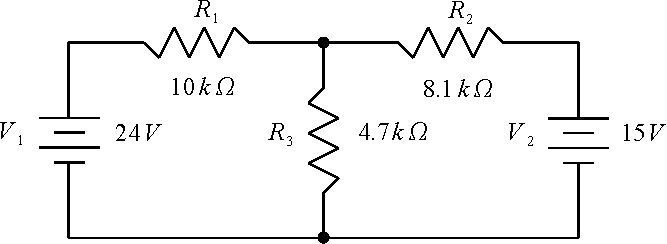
\includegraphics[scale=1]{./figures/circuit.pdf}
\caption{Schematic: ``Multiple dc sources''}
\label{fig:Circuit}
\end{figure}

\begin{table}
\centering
\caption{Netlist: ``Multiple dc sources''}
\label{tab:Netlist}
\begin{tabular}{c}
  \toprule
  v1 1 0 dc 24 \\
  v2 3 0 dc 15 \\
  r1 1 2 10k \\
  r2 2 3 8.1k \\
  r3 2 0 4.7k \\
\bottomrule
\end{tabular}
\end{table}

We believe that---through the right combination of conceptual modeling, abstract language, and graphical visualization---the art of IACS can be transformed into a science and an engineering discipline.  We are not, however, suggesting that the approach we propose is an automated solution or a template for patent application drafting.  In fact, we believe that {\em more} creative input from practitioners would be required (though more profitably applied), for the true problem would be laid bare.

Even with all the power of the modern computer, there is no substitute for human innovation to tackle unsolved problems.  But as leverage for creativity, the combination of modeling, abstract language and computer tools has forged the technological world we see today. The next section introduces conceptual graphs as an ideal abstract language, both for modeling and for computer-assisted analysis.

\section{Conceptual Graphs}\label{sec:CGprimer}

%\epigraph{You have to learn the rules of the game. And then you have to play better than anyone else.}{Albert Einstein}
\epigraph{Most of the fundamental ideas of science are essentially simple, and may, as a rule, be expressed in a language comprehensible to everyone.}{Albert Einstein}


Conceptual graphs\footnote{See, e.g., \cite{Sowa84,Sowa00,Sowa08,Chein09}. An online course is available at \url{http://cg.huminf.aau.dk}. A softcopy of \cite{Sowa08} is available at \url{http://www.jfsowa.com/cg/cg_hbook.pdf}. Several illustrative examples can be found at \url{http://www.jfsowa.com/cg/cgexampw.htm}.}, a notation for representing knowledge, promote logical analysis and synthesis. A kind of graphical logic, CGs are sufficiently friendly to be read by novices, but precise enough to be read by computers. They are actively studied,\footcite{Chein09} closely related to the {\em semantic web},\footnote{An early vision for the semantic web was ``{...}~an evolution of a Web that consisted largely of documents for humans to read to one that included data and information for computers to manipulate.'' (\url{http://eprints.ecs.soton.ac.uk/12614/1/Semantic_Web_Revisted.pdf}~). For the relationship between the sematic web and CGs see \url{http://www.w3.org/DesignIssues/CG.html}.} and are the core of the Common Logic ISO standard.\footnote{See, e.g., \url{http://staff.um.edu.mt/cabe2/lectures/webscience/docs/polovina_07.pdf}.}

For our purposes, it is best to introduce CGs through examples. Necessarily we will omit many technical details, but we aim to traverse a broad landscape, rather than dwell on local points of interest. Figure~\ref{fig:[cat]} shows the simplest possible graph, a single concept: a cat.
%
\begin{figure}
\centering

\includegraphics[scale=1]{./figures/cat.pdf}
\caption{A concept}
\label{fig:[cat]}
\end{figure}
%
The graph asserts the existence of the {\em concept} of a cat. It stands for the {\em abstract idea} of a cat, rather than any particular cat. The graph of figure~\ref{fig:[cat:catbert]}, on the other hand, asserts that a particular cat, `Catbert', exists.

\begin{figure}
\centering

\includegraphics[scale=1]{./figures/catbert.pdf}
\caption{An instance of a concept}
\label{fig:[cat:catbert]}
\end{figure}

Along with concepts and instances, {\em relations} allow us to build non-trivial graphs. Figure~\ref{fig:catbertOnMat} uses two relations, `On' and `Attr' (Attribute), allowing us to assert the knowledge that ``A cat, Catbert, is on a mat, and the mat has a color, and that color is green''. Or, more eloquently, ``Catbert, the cat, is on a green mat.''

\begin{figure}
\centering
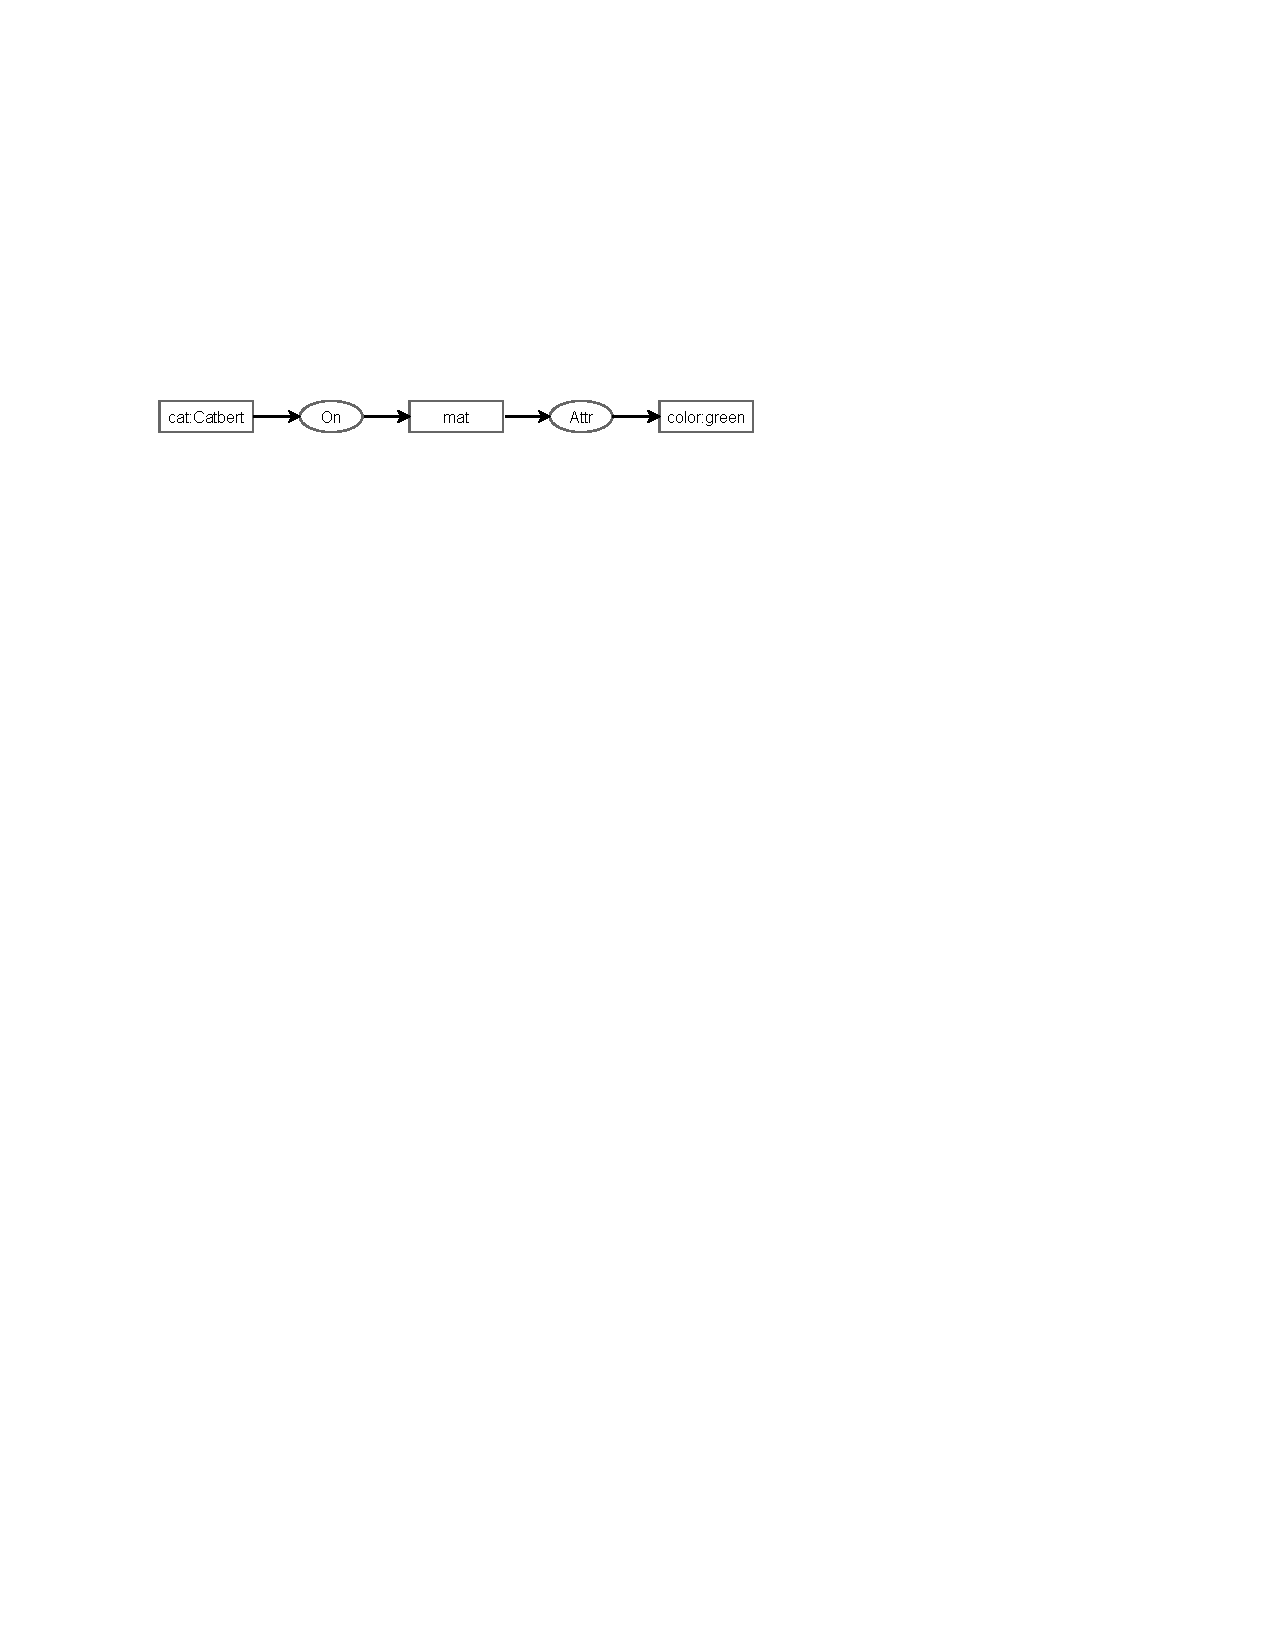
\includegraphics[scale=1]{./figures/catbertGreenMat.pdf}
\caption{A graph with relations}
\label{fig:catbertOnMat}
\end{figure}


An important aspect of conceptual graphs is that everything in the world of discourse must be declared and organized by type. In CGs this is known as the {\em support} for the graph, and forms a simple ontology. For example, we already know that `Catbert' is a type of `cat', but we might also declare that `cat' is a type of `animal', and that `On' is a type of `Position'. Figure~\ref{fig:ontology} graphically shows an example ontology.

\begin{figure}
\centering
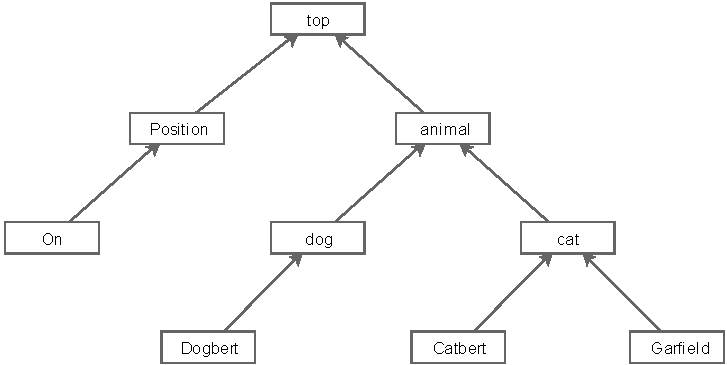
\includegraphics[scale=1]{./figures/ontology.pdf}
\caption{The support for a graph}
\label{fig:ontology}
\end{figure}

Although we have the basic material required to begin our examination of IACS, it is worthwhile, though we gloss over some detail, to preview the more advanced idea of {\em projection}. Say figure~\ref{fig:catbertOnMat} asserts knowledge about our world (a fact-graph), and we have a query---``Is an animal on the mat?''. In CGs, we form a {\em query} graph, as shown in figure~\ref{fig:animalOnMat}.

\begin{figure}
\centering
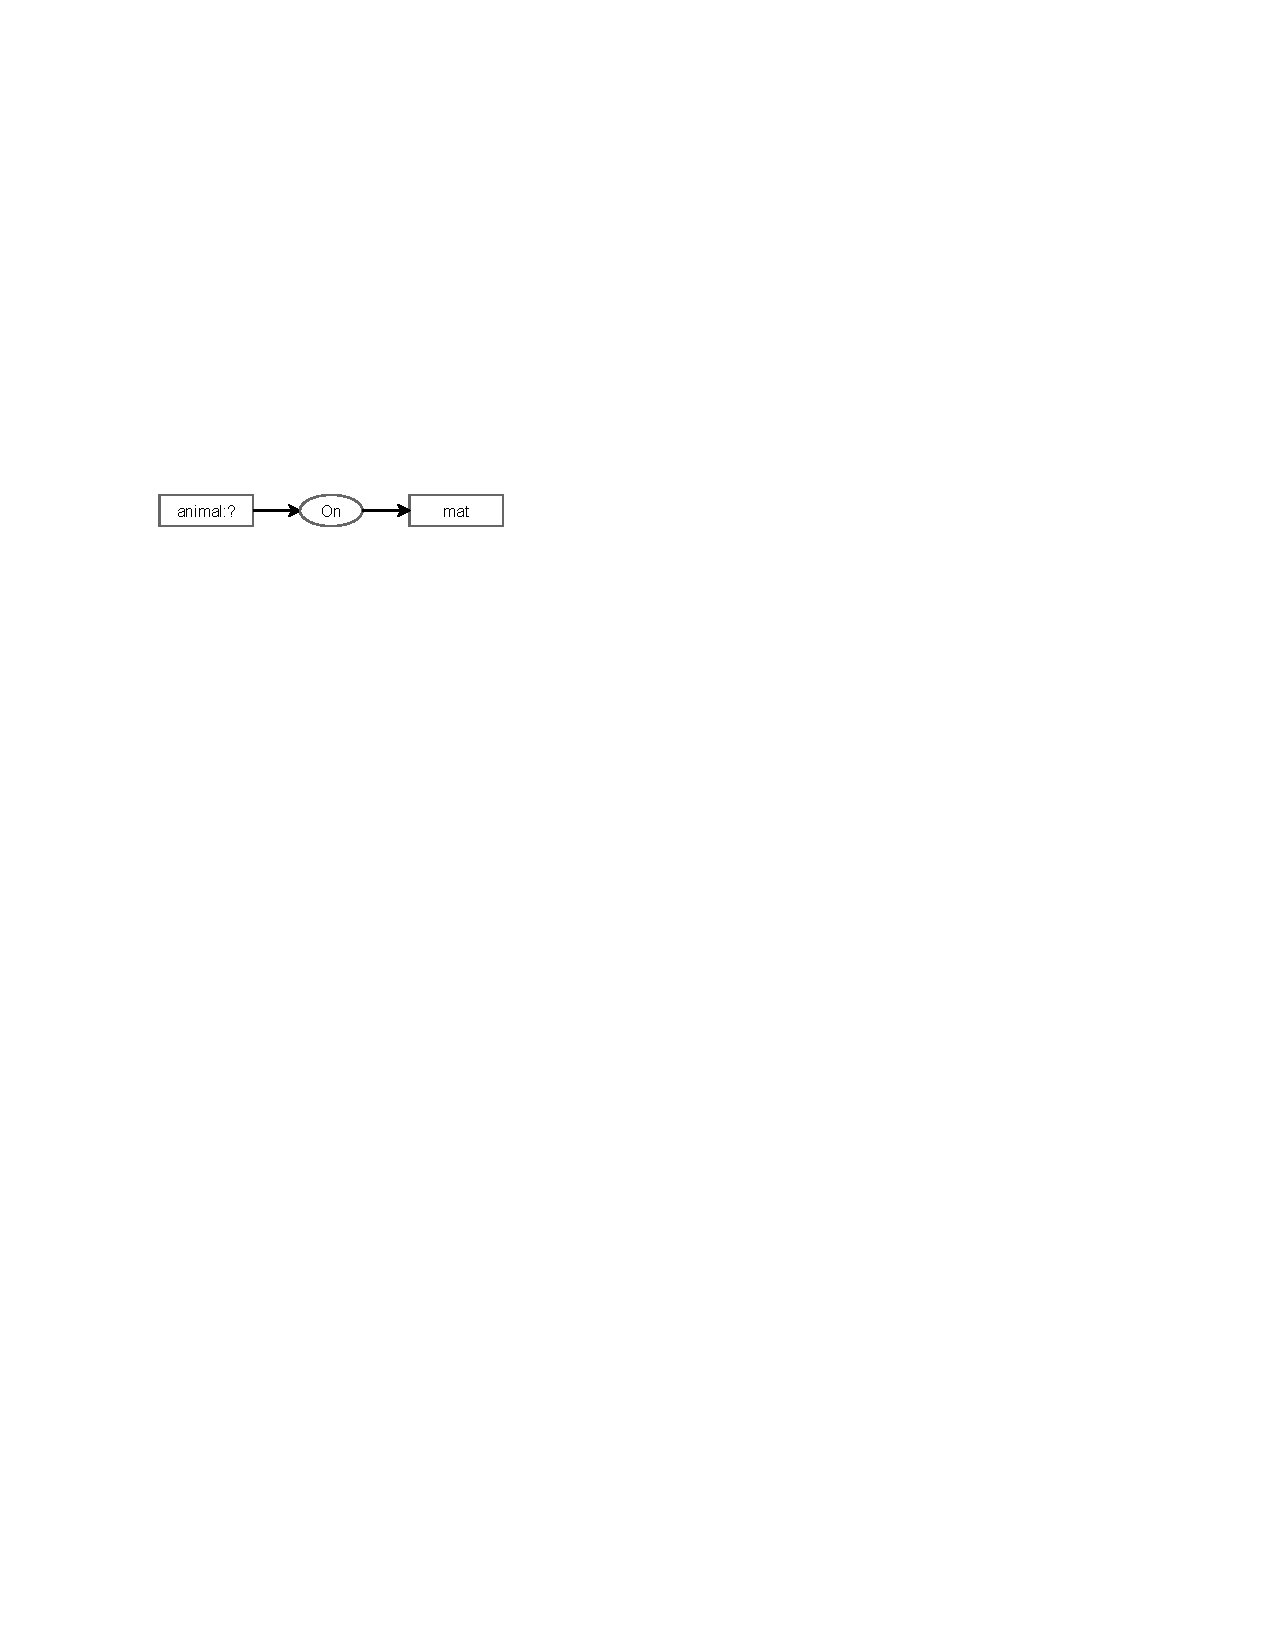
\includegraphics[scale=1]{./figures/animalOnMat.pdf}
\caption{A query graph}
\label{fig:animalOnMat}
\end{figure}

The query is answered by projecting the query graph into the fact graph. A projection looks to see if the query graph, {\em or any specialization of the query graph}, can be found in the fact graph. In this case, since `Catbert' is a specialization of `cat', which, in turn, is a specialization `animal' (see figure~\ref{fig:ontology}), a specialization of the query graph can indeed be found. That is, the projection is as shown in figure~\ref{fig:projection}, and, indeed, the answer to the query is that ``Catbert, the cat, is on the mat''.

\begin{figure}
\centering
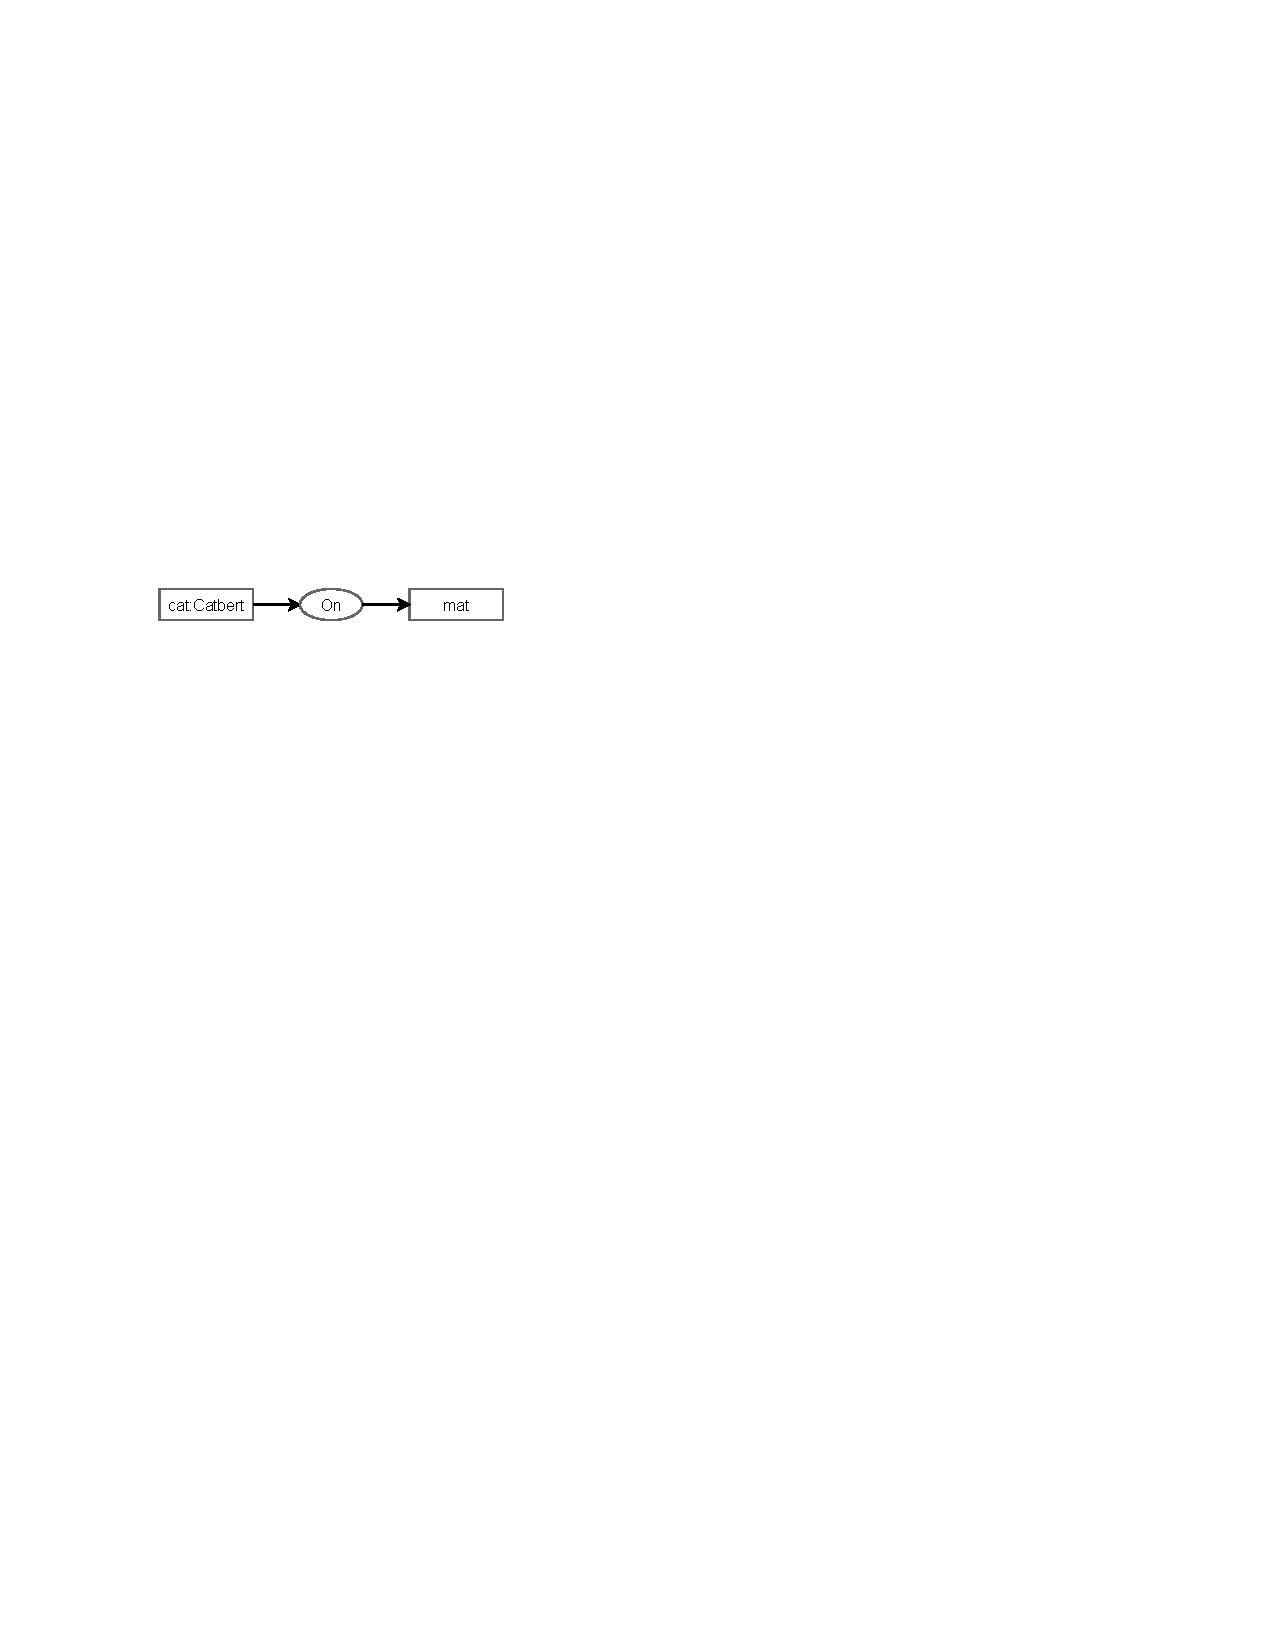
\includegraphics[scale=1]{./figures/catbertOnMat.pdf}
\caption{An answer graph}
\label{fig:projection}
\end{figure}

With the core principles at hand, the next section introduces conceptual graphs as an ideal abstract language for IACS modeling and computer tools.

\section{Inventions}\label{sec:inventions}

%\epigraph{You shouldn't write {\em anything} first. Figure out what the invention is, and then you can write whatever you want.}{Ronald D. Slusky}
%\epigraph{For patent lawyers, however, an invention is not something physical, but a concept}{Slusky}
%\epigraph{One of the principal objects of research in my department of knowledge is to find the point of view from which the subject appears in the greatest simplicity.}{Josiah Willard Gibbs}
\epigraph{We still do not know one thousandth of one percent of what nature has revealed to us.}{Albert Einstein}

Our most basic notion is that conceptual graphs can represent prior art and embodiments; and, subsequently, that a claim (also a CG) can be synthesized by manipulating CGs (this is the basis of the example workflow in appendix~\ref{sec:workflow}). For example, figure~\ref{fig:cgPaEmbExample} shows two graphs representing (a) prior art, and (b), an embodiment. The upper graph, (a), represents the idea that a hull (of a paddle steamer say) has a paddle-wheel and a steam-engine as parts, and that the steam-engine drives the paddle-wheel. The lower graph, \ref{fig:cgPaEmbExample}(b), relates to a microwave oven and asserts that a cavity is the location of food, and the recipient of an energy source.

\begin{figure}
  \centering
  \subfloat[~]{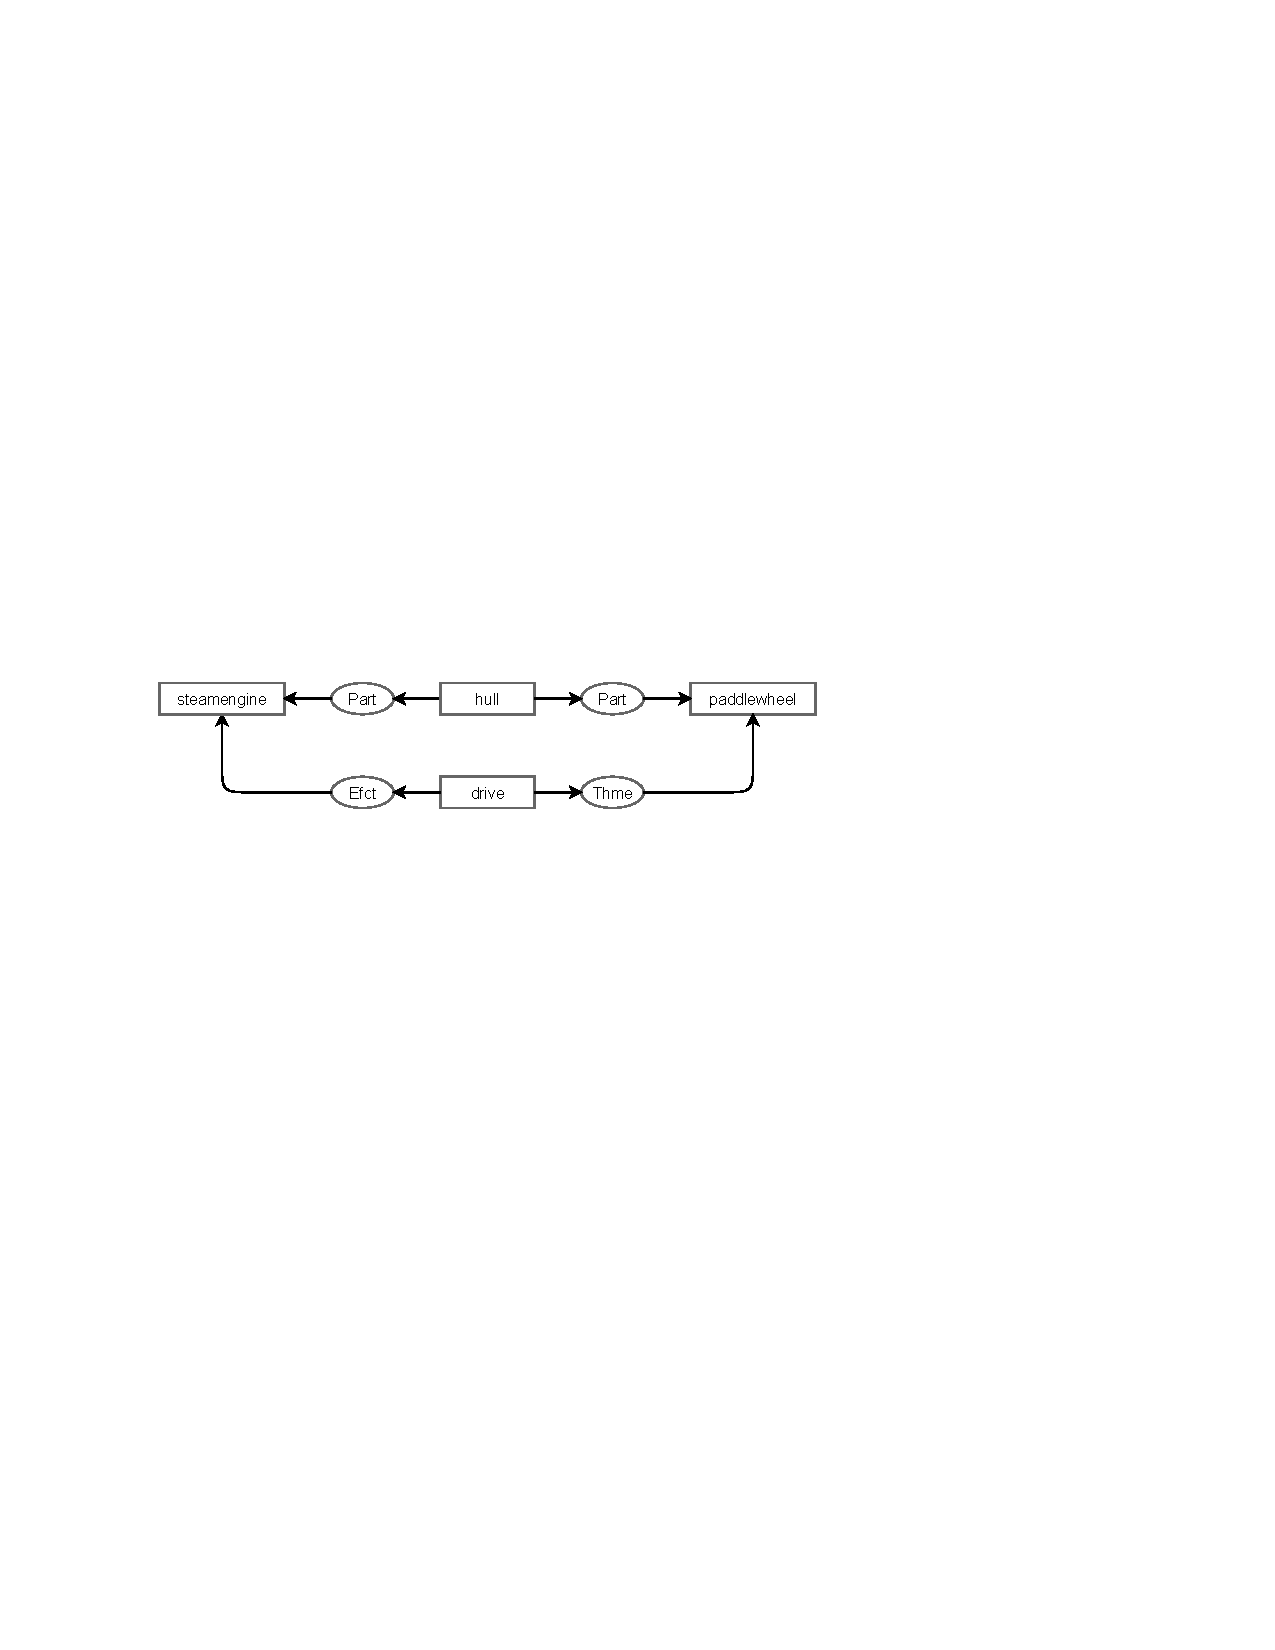
\includegraphics[scale=1]{./figures/paddlesteamer.pdf}} \\
  \subfloat[~]{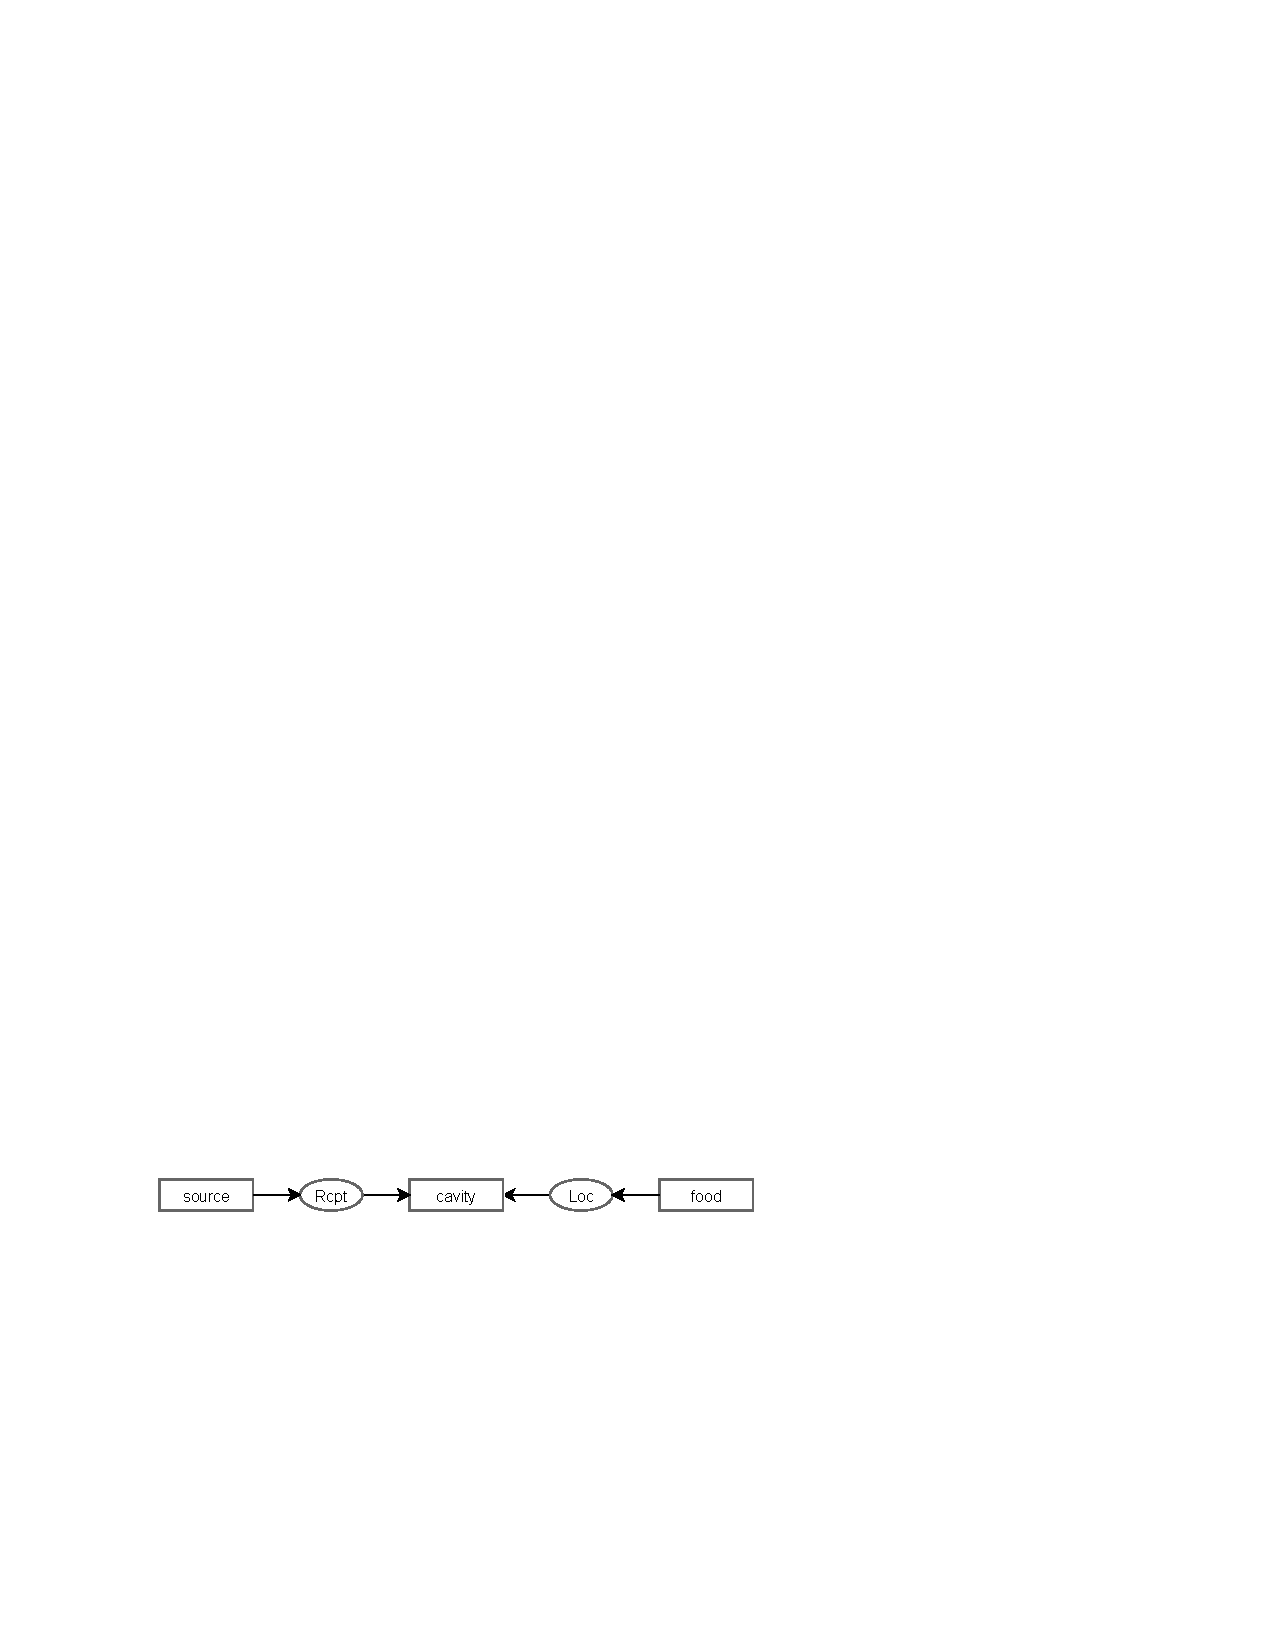
\includegraphics[scale=1]{./figures/microwavePA.pdf}}
\caption{(a) paddle steamer, (b) microwave oven}
\label{fig:cgPaEmbExample}
\end{figure}

These are our most complex graphs so far, and deserve further explanation. When moving from a concept to a relation in the direction of the arrow, we may think to ourselves, ``has''.\footnote{There are various ways of converting graphs into natural language; some will be more `natural' than others, depending on the relation (see, e.g., \url{http://cg.huminf.aau.dk/Module_I/1037.html}~). The ``cat on mat'' graph (figure~\ref{fig:catbertOnMat}), for example, does not work well with the recipe that follows. In all cases though, the user can define precisely what a relation means, and the best way for it to be read. Thus, the user is both their own lexicographer, and their own linguist.} So, in the top line of figure~\ref{fig:cgPaEmbExample}(a), ``hull has part steamengine'' and ``hull has part paddlewheel''. Alternatively, read in the opposite direction (against the direction of the arrows), we may think, ``is''. For example, ``steamengine is part of hull'' and ``paddlewheel is part of hull''.

Several new relationships have been introduced. Typically, though it is more a matter of style than logic, we choose to select from a limited palette of relations.\footnote{Although, there is support for using a limited number of relations in theoretical linguistics. A thematic relation expresses the role that a noun-phrase plays with respect to a verb (\url{http://en.wikipedia.org/wiki/Thematic_relation}). For a treatment more closely related to CG, see \url{http://www.jfsowa.com/ontology/thematic.htm}. For a convenient list of relations,  see  \url{http://cg.huminf.aau.dk/Module_I/1142.html}.} For example, `Efct' is an abbreviation of `Effector' and means ``An active entity that initiates an action''---so, from graph~\ref{fig:cgPaEmbExample}(a), `drive has effector steamengine'. Moreover, `Thme' is an abbreviation of ``Theme'', and means ``A participant that may be moved, said, or experienced, but is not structurally changed.''---thus, ``drive has theme paddlewheel''.

 Though we will use both graphs again in latter sections, the most important point at this stage is that {\em graphs represent knowledge}. In artificial intelligence parlance, CGs are a form of ``knowledge representation''.\footnote{See, e.g., \url{http://en.wikipedia.org/wiki/Knowledge_representation_and_reasoning}.} In other words, graphs assert facts about the world of interest (inventions); furthermore, as we show below, they do so in a very useful way.

\section{Generalization and Specialization}

\epigraph{Everything should be made as simple as possible, but not simpler.}{Albert Einstein}

Invention analysis and claim synthesis is, in large part, an exercise in optimized generalization and specialization (see, for example, the workflow in appendix~\ref{sec:workflow}). Just as a concept is a generalization (from specific instances), so too are claims generalizations of embodiments, and dependent claims specializations of independent claims. In conceptual graphs there are only three fundamental operations---two of which are specialization and generalization~\footcite[The third is {\em equivalence}, which is important, but not required here]{Sowa08}. Thus, we begin to see a close connection between IACS and CGs.

Specialization itself has two flavors, {\em join} and {\em restrict}. The join operation specializes a graph by attaching (joining) another graph to it. For instance, if we have a yellow pencil (a pencil with a characteristic (`Chrc') color, yellow---figure~\ref{fig:specialization1}(a)) and a pencil with an eraser (figure~\ref{fig:specialization1}(b)), then we can join the two graphs to find a third graph (figure~\ref{fig:specialization1}(c)), which is a specialization of both (a) and (b). That is, (a) is specialized in (c), because (c) asserts not just any yellow pencil, but a pencil with an eraser.

\begin{figure}
  \centering
  \subfloat[~]{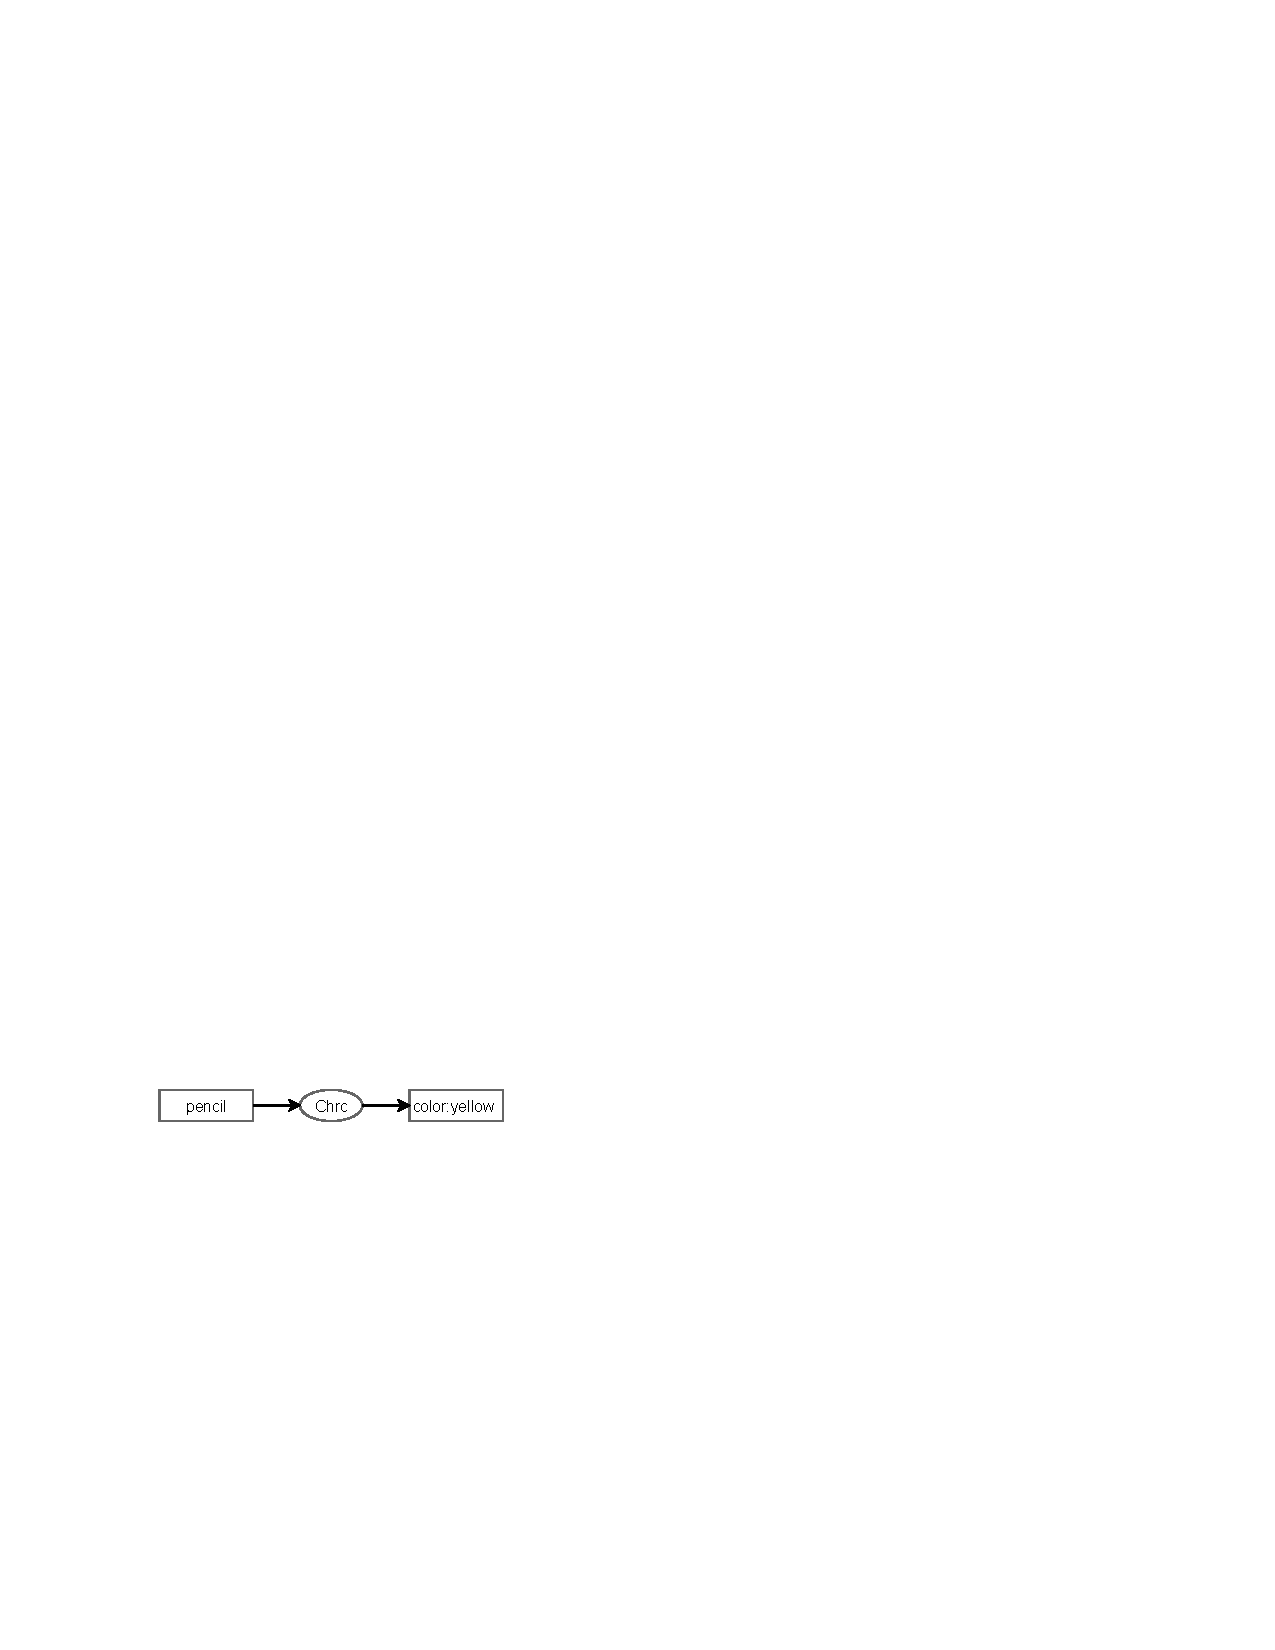
\includegraphics[scale=1]{./figures/SpecA.pdf}} \\
  \subfloat[~]{
\includegraphics[scale=1]{./figures/SpecB.pdf}} \\
  \subfloat[~]{
\includegraphics[scale=1]{./figures/SpecB2.pdf}}
  \caption{Specializing by joining}
  \label{fig:specialization1}
\end{figure}

The restrict operation refers to the ontology of concepts and relations. For instance, if we have a pencil with a rod (figure~\ref{fig:specialization2}(a)), then we can specialize this graph by restricting the rod to a graphite rod (figure~\ref{fig:specialization2}(b)).

\begin{figure}
  \centering
  \subfloat[~]{
\includegraphics[scale=1]{./figures/SpecC.pdf}} \\
  \subfloat[~]{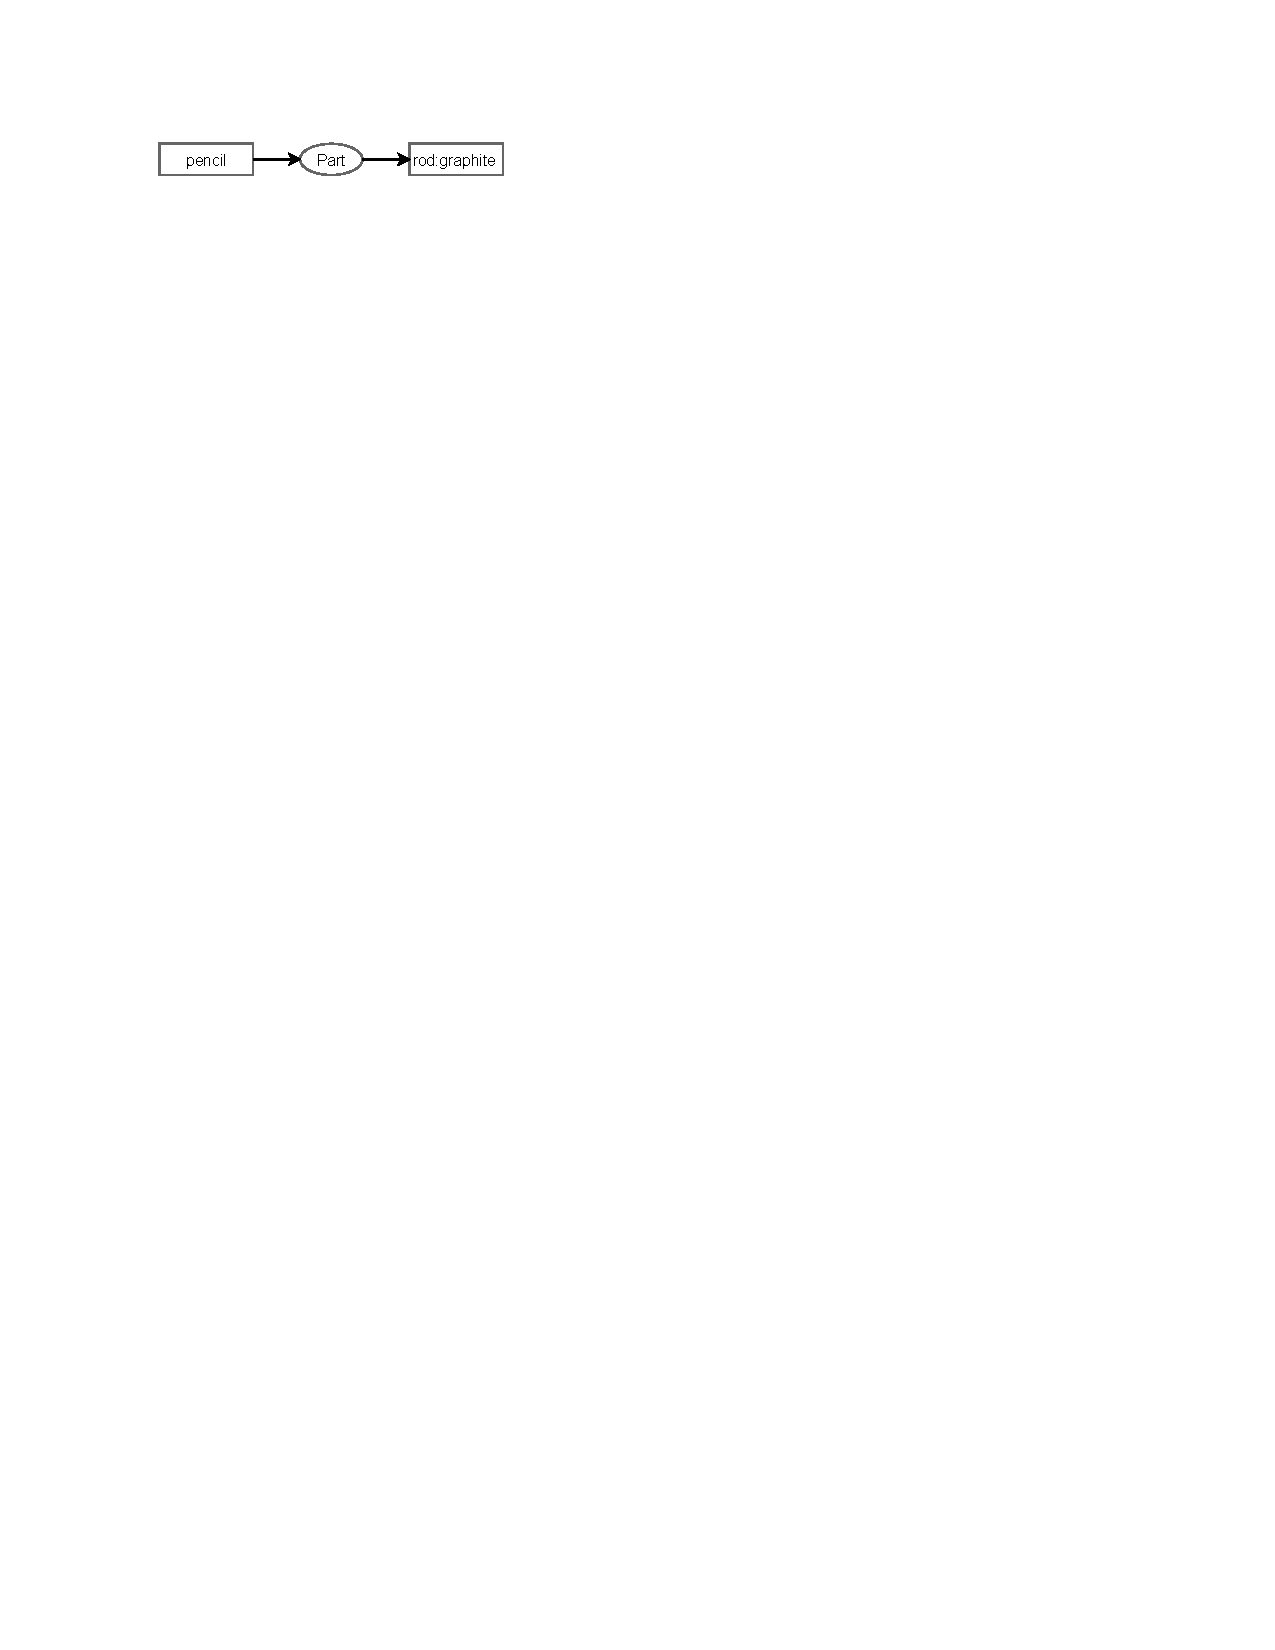
\includegraphics[scale=1]{./figures/SpecD.pdf}}
  \caption{Specializing by restricting concepts}
  \label{fig:specialization2}
\end{figure}

We may also restrict relations. Figure~\ref{fig:specialization3}(a) asserts a pencil with a characteristic (`Chrc') cylindrical (`cyl') geometry (`geom'), that has a rod with some orientation (`Orient') to the geometry. Figure~\ref{fig:specialization3}(b) specializes the orientation to be coaxial (`Coax')---that is, the pencil's rod is coaxial with its cylindrical geometry.

\begin{figure}
  \centering
  \subfloat[~]{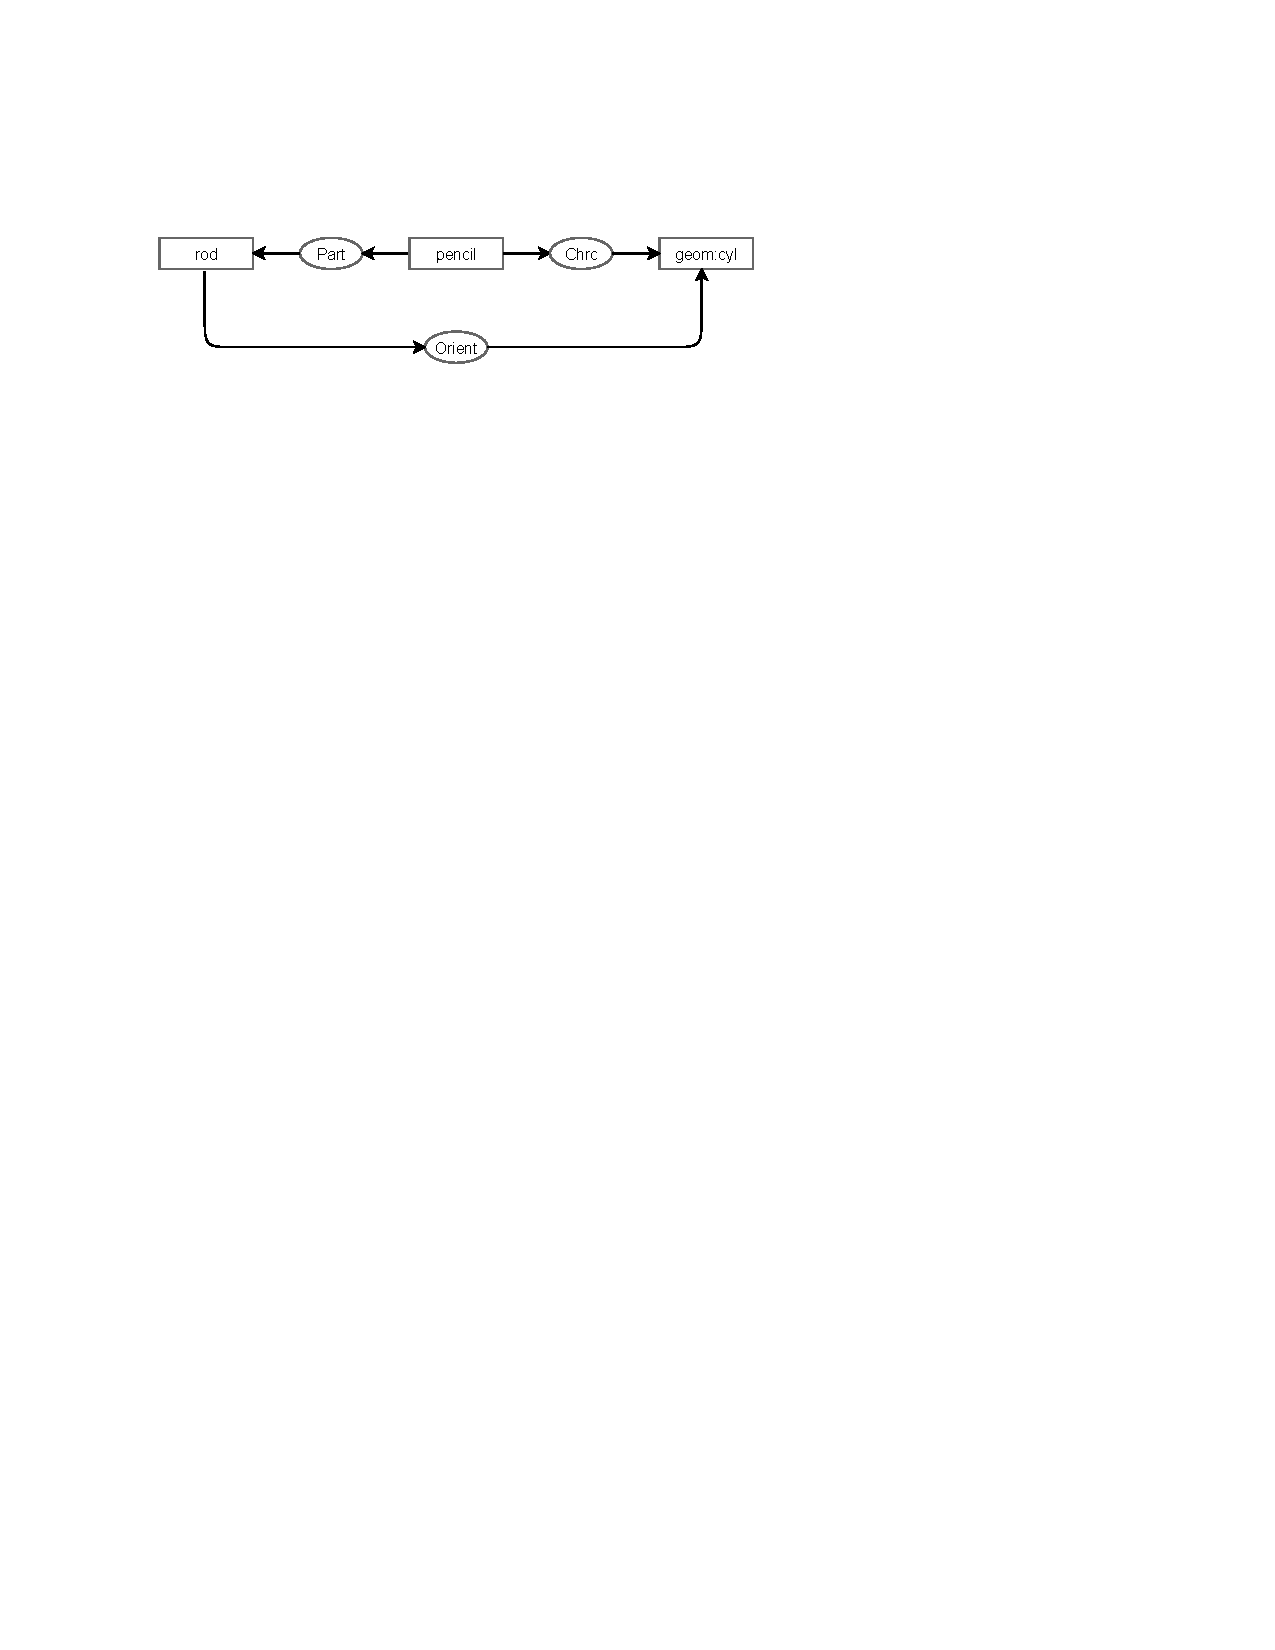
\includegraphics[scale=1]{./figures/SpecE.pdf}} \\
  \subfloat[~]{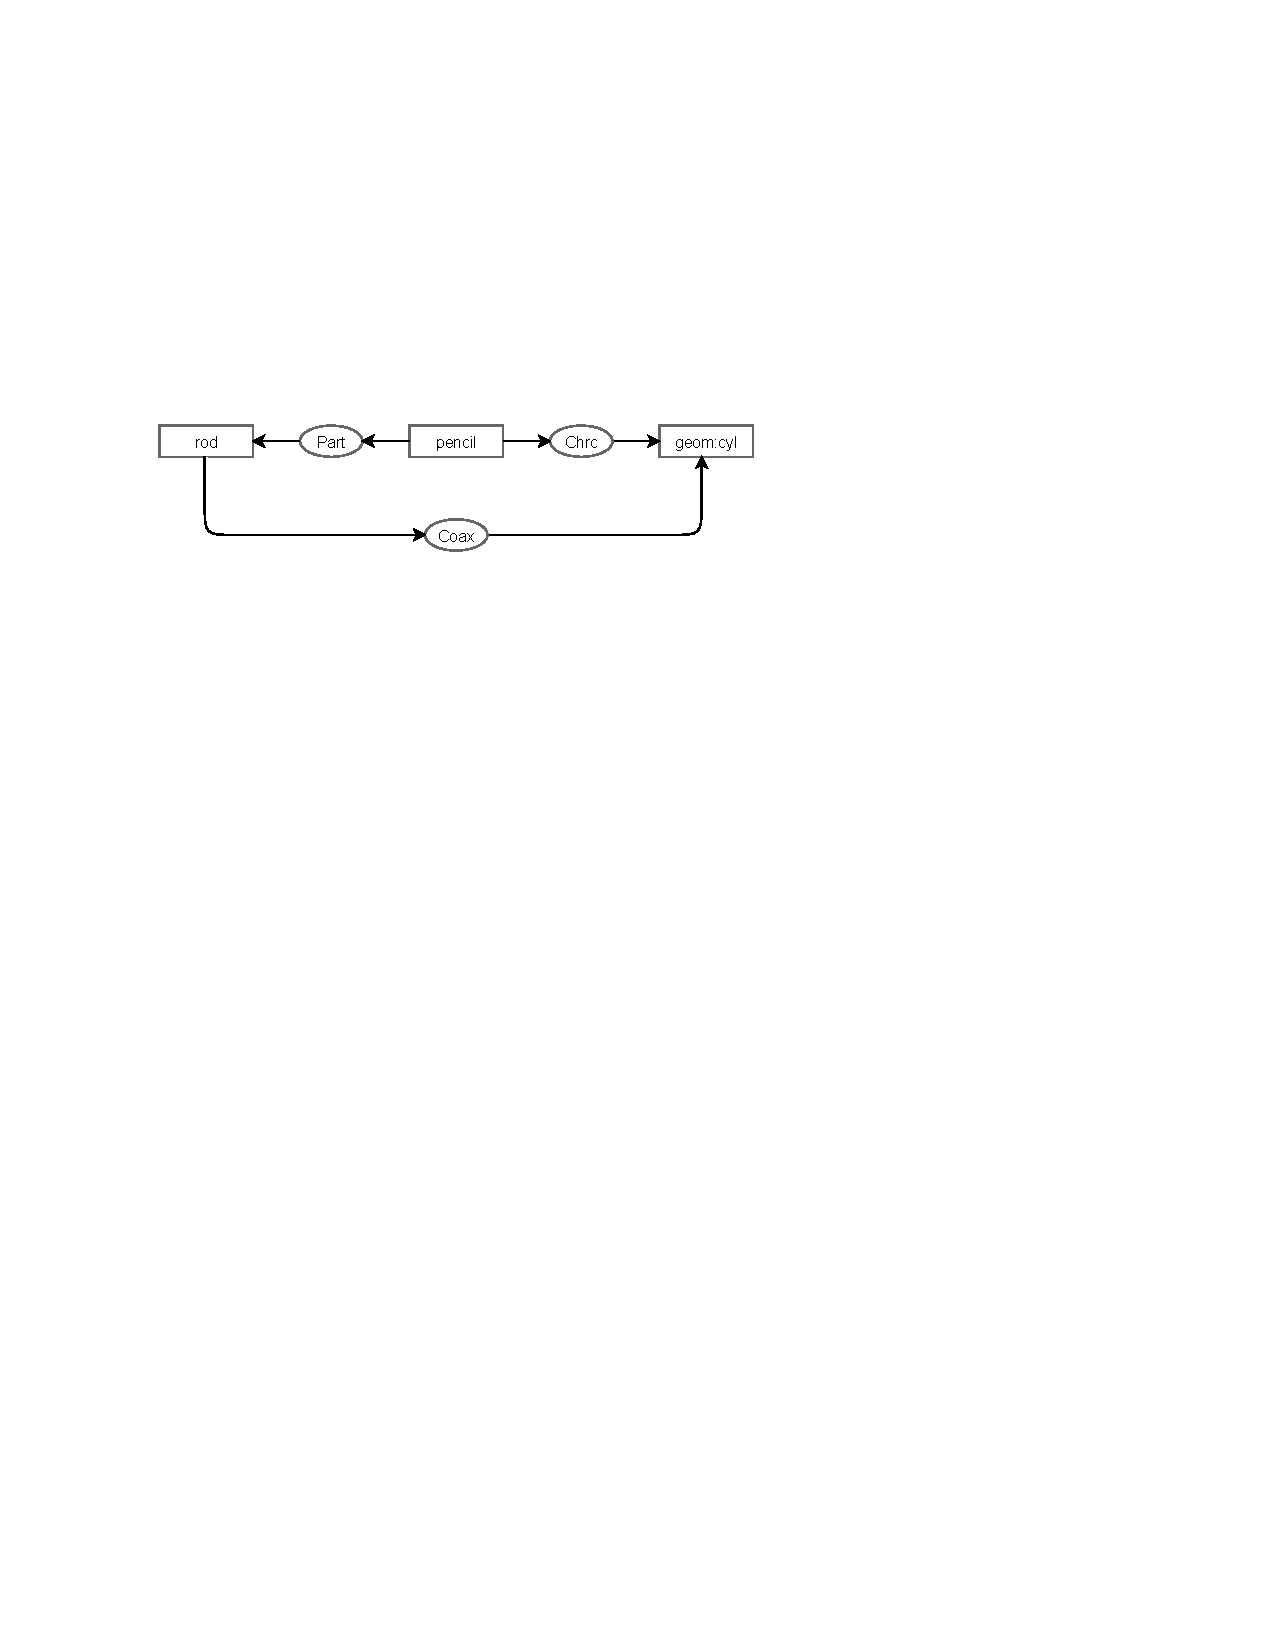
\includegraphics[scale=1]{./figures/SpecF.pdf}}
  \caption{Specializing by restricting relations}
  \label{fig:specialization3}
\end{figure}

To further emphasize the connection of specialization with IACS, we refer to the following quote~\footcite[Chapter~9]{Slusky07}:
%
\begin{quote}
A fallback feature claim can further limit the subject matter of its parent by (a) adding one or more additional elements to the elements contained in the parent claim; (b) particularizing an already recited element in the parent claim; or (c) particularizing the relationship between already recited elements.
\end{quote}
%
Here, (a) corresponds to a CG `join', (b) corresponds to a CG `restrict' of a concept, and (c) corresponds to a CG `restrict' of a relation.

The inverse of specialization is generalization. The inverse of `join' is `detach'---that is, moving from figure~\ref{fig:specialization1}(c) to the combination of figure~\ref{fig:specialization1}(a) and figure~\ref{fig:specialization1}(b). The inverse of `restrict' is `unrestrict', that is, moving from figure~\ref{fig:specialization2}(b) to figure~\ref{fig:specialization2}(a). As with specialization, the CG operations of `detach' and `unrestrict' have their counterparts in IACS---namely `prune' and `distill'.~\footcite[Chapter~4]{Slusky07}

Generalization and specialization are native concepts for conceptual graphs, just as they are core elements of IACS. In the next section we see that generalization and specialization are key to inference, and, in turn, to the IACS notion of ``reads-on''.

\newpage

\section{Inference}\label{sec:inference}

%\epigraph{Judges must beware of hard constructions and strained inferences, for there is no worse torture than that of laws.}{Francis Bacon}
\epigraph{Logic will get you from A to B. Imagination will take you everywhere.}{Albert Einstein}

Having introduced the elemental CG operations of specialization and generalization, we turn to more complex operations.\footnote{All of which can ultimately be decomposed into specialization, generalization, and equivalence. Examples of their use appear in the example workflow in appendix~\ref{sec:workflow}.} Broadly speaking, each topic in this section is a kind of {\em inference}, in the sense that we draw a conclusion that is implicit in the knowledge at hand.

First, we recall the idea of projection, introduced in section~\ref{sec:CGprimer} to answer a query, to address the IACS ideas of novelty and infringement. Second, we consider a special kind of graph-joining that has application to prior art and ``obviousness''. Finally, the CG notion of `least-generalization' is introduced.

\subsection{Novelty and Infringement}

One of the first pieces of {\em legalese} an engineer learns is ``reads-on''---for example, whether a claim reads-on a piece of prior art or a competitor's product. Intuitively it is straightforward: a claim reads-on some thing if that thing falls within the scope of the claim.

More specifically, a claim reads-on a thing if we can find the claimed concept---{\em or any specialization of the claimed concept}---within the concept of the thing. So, for instance, if a claim's concept is a ``writing implement'', then it will read-on specializations such as pens, pencils and chalk. This is {\em precisely} the idea of projection that was introduced with conceptual graphs in section~\ref{sec:CGprimer}.

For example, consider the graph in figure~\ref{fig:car}, which shows part of a claim for a car with a chassis, engine, and wheels, with the engine driving the wheels. Furthermore, say that the graph of figure~\ref{fig:cgPaEmbExample}(a) represents the prior art. If, according to our ontology (not shown), `steamengine' is a specialization of `engine', `hull' is specialization of `chassis', and `paddlewheel' is a specialization of `wheel', then figure~\ref{fig:car} projects into figure~\ref{fig:cgPaEmbExample}(a), and we say that the claim reads on the prior art.

\begin{figure}
\centering
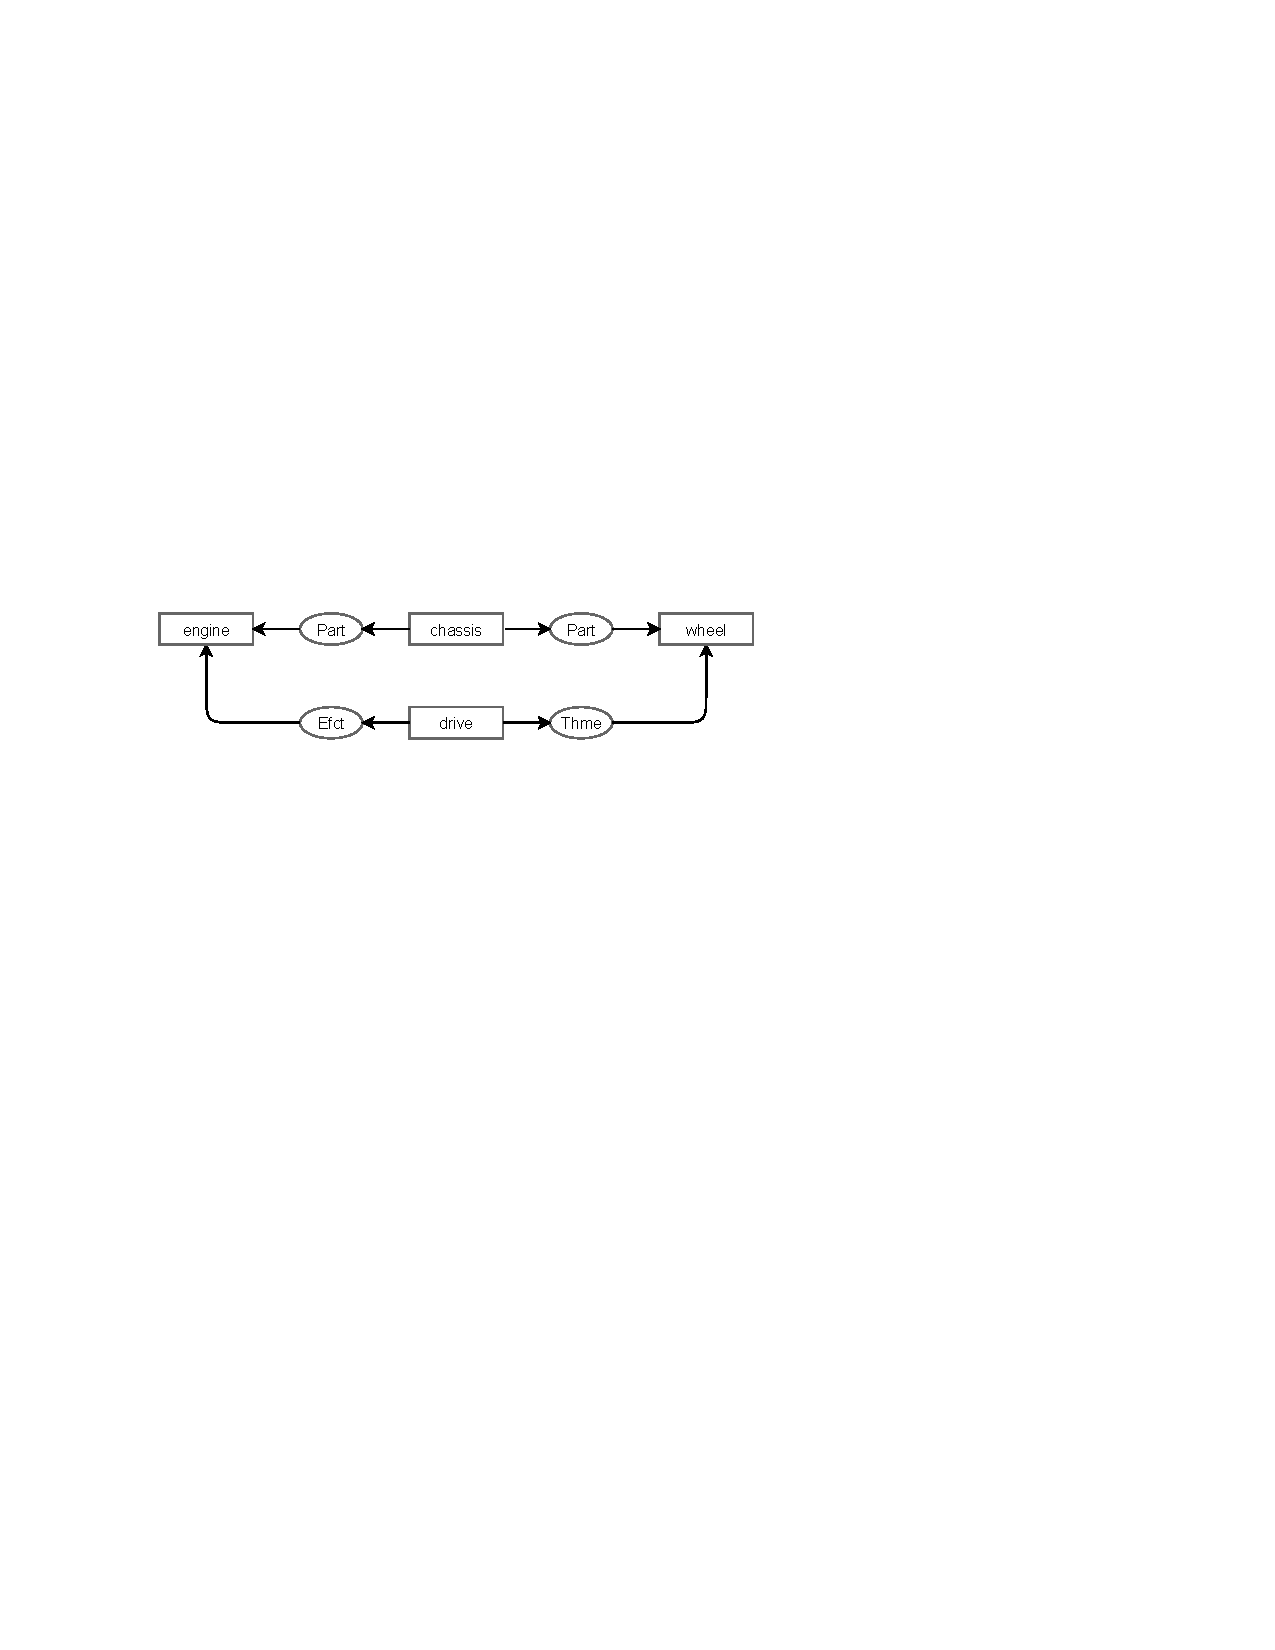
\includegraphics[scale=1]{./figures/car.pdf}
\caption{A `car' that projects on the `steamboat' of figure~\ref{fig:cgPaEmbExample}(a)}
\label{fig:car}
\end{figure}

Thus projection can be applied as a test for novelty. Similarly, whether a claim projects onto a competitor's product (i.e., whether the claim's concept, or its specialization, can be found within the product) is a test for infringement.\footnote{It is instructive to pause to note the effect of adding limitations to a claim. In CG terms a limitation is a specialization; and so, specializing a claim means it is less likely to project into either the prior art or a competing product.}

\subsection{Obviousness}

Sowa has the following to say about the CG operation of `maximal join':~\footcite{Sowa08}
%
\begin{quote}
A multistep combination, called a maximal join, is used to determine the extent of the
unifiable overlap between two CGs.
\end{quote}
%
To explain further we move straight to an example. Figure~\ref{fig:maxjoin}(a) shows a special ink (``\#7'') that has some interesting attribute, and that is known to be in the prior art. Figure~\ref{fig:maxjoin}(b) shows that black ink (ink with a characteristic of `color', the color being black) is also in the prior art. Figure~\ref{fig:maxjoin}(c) shows a maximal join of (a) and (b), where the graphs are joined at the greatest specialization of their common concept (i.e., ink \#7). Thus, the maximal join of (a) and (b) asserts that if ink \#7 is in the prior art and black ink is in the prior art, then black ink \#7 is, by inference, also in the prior art. Or, to put it another way, this fact is {\em implicitly} obvious.

\begin{figure}
  \centering
  \subfloat[~]{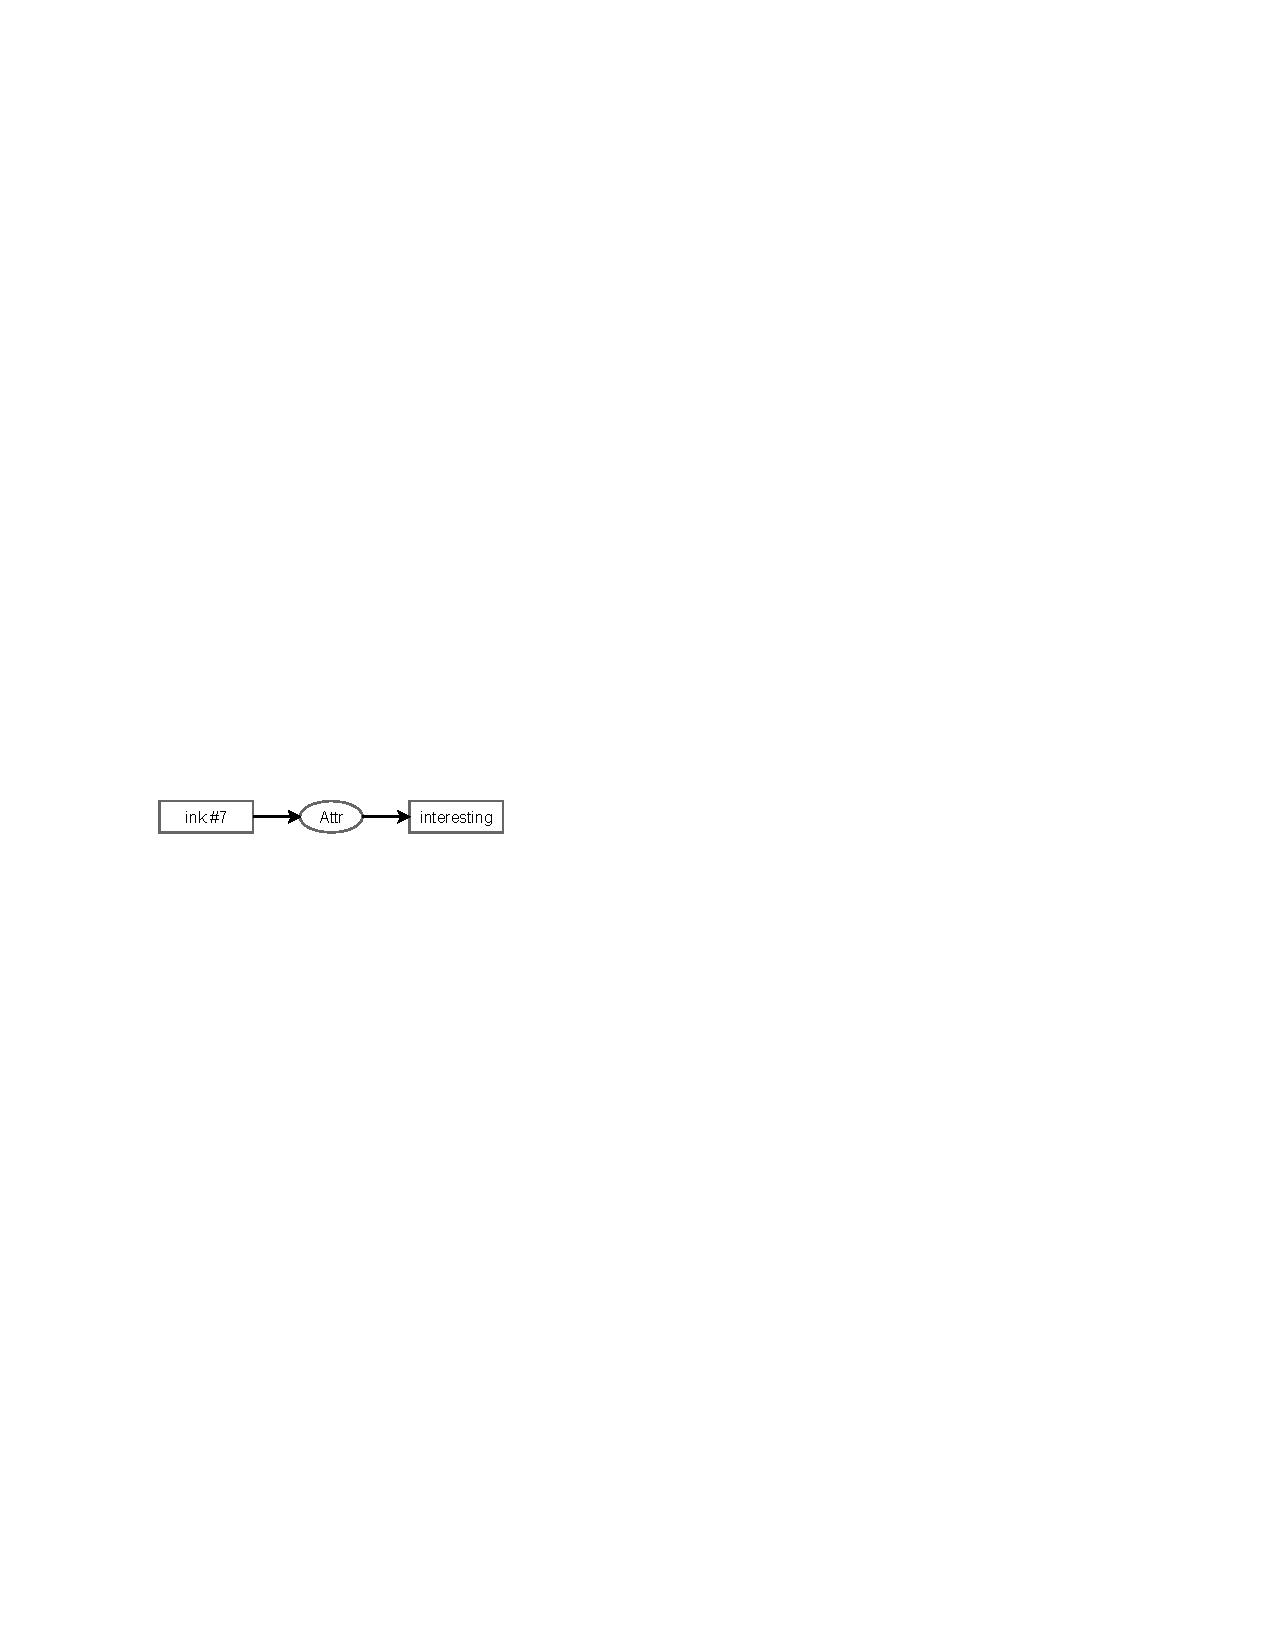
\includegraphics[scale=1]{./figures/specialink.pdf}} \\
  \subfloat[~]{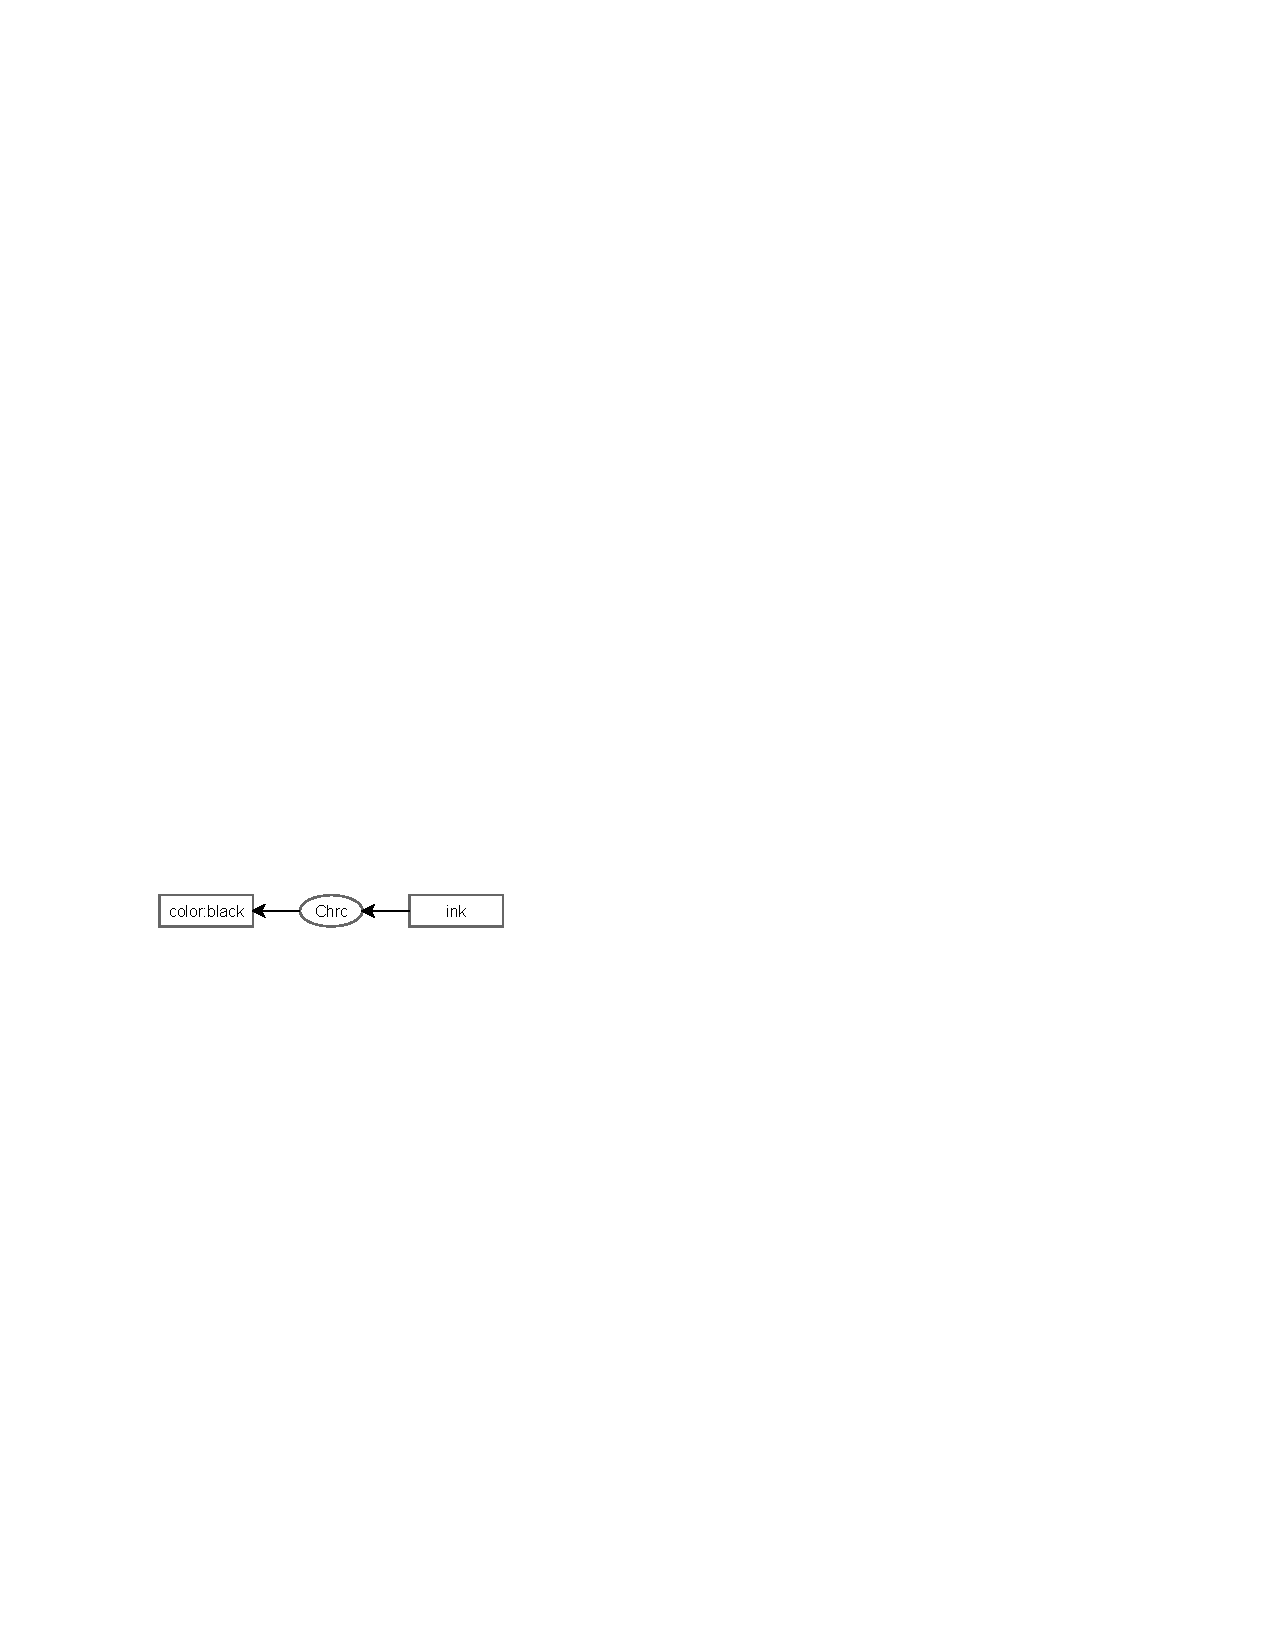
\includegraphics[scale=1]{./figures/blackink.pdf}} \\
  \subfloat[~]{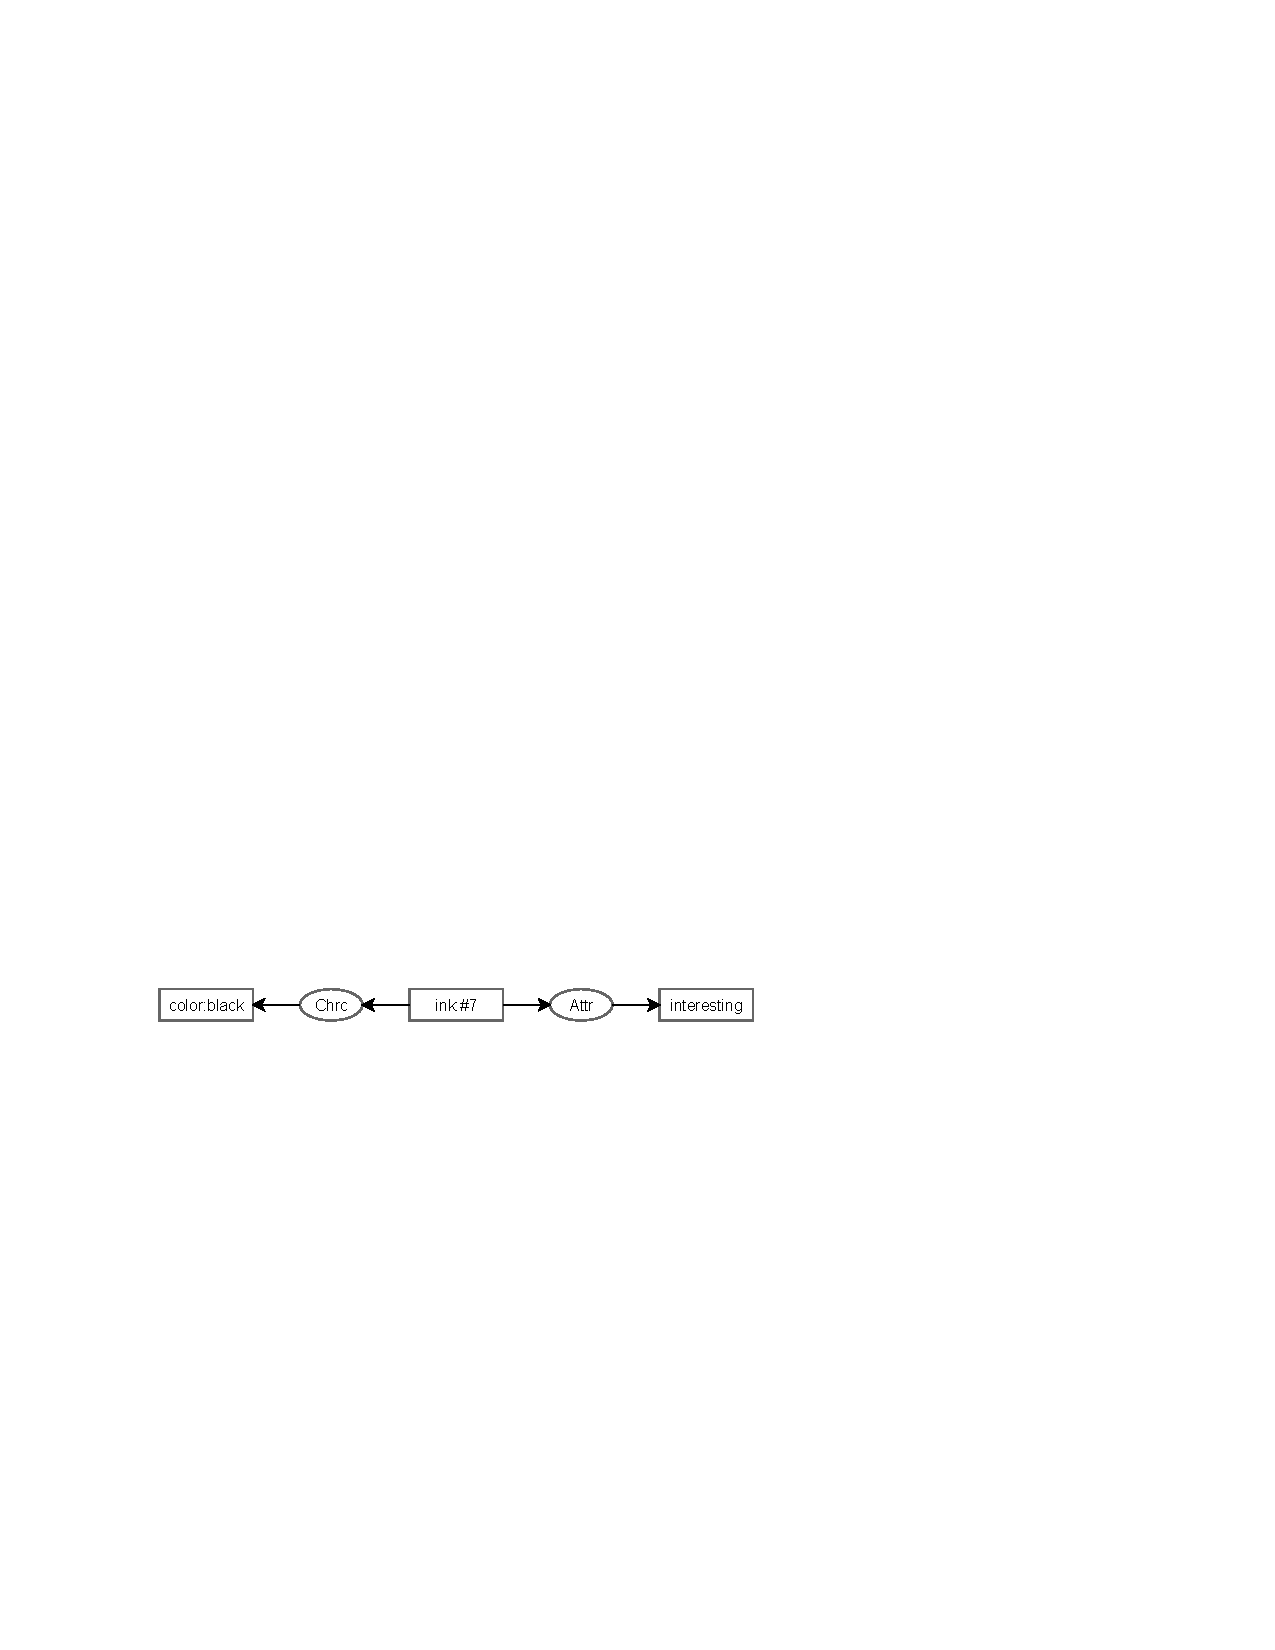
\includegraphics[scale=1]{./figures/maxjoin.pdf}}
\caption{(a) special ink, (b) black ink, (c) special black ink}
\label{fig:maxjoin}
\end{figure}

\subsection{Least Generalization}\label{sec:leastgen}

The least generalization of two (or more) graphs is a graph that is a generalization of both, but is less generalized (i.e., more specialized) than any other possible generalization.\footnote{See, e.g., \cite{Sowa84,Sowa00,Sowa08,Chein09}.} Again, it is easiest to understand via example.

Figure~\ref{fig:leastgen}(a) shows part of an embodiment for a push-button telephone.\footcite[Chapter~4]{Slusky07} Focussing on the `selection' concept, `selection' has agent\footnote{An active animate entity that voluntarily initiates an act. \url{http://cg.huminf.aau.dk/Module_I/1142.html\#Agnt}.} (Agnt) `user', and instrument\footnote{An instrument used in an act. The instrument is not changed by the activity. \url{http://cg.huminf.aau.dk/Module_I/1142.html\#Inst}.} (Inst) `button'. The result of the selection is a `tone', and the instrument of the tone is an oscillator. In natural language, we might say that a user makes a selection using a button, with a resulting tone generated by an oscillator. Figure~\ref{fig:leastgen}(b) shows a similar situation, except in this case the tone is generated by a parrot, and the user's selection is made by telepathy.\footcite[See example far-fetched embodiment in Chapter~4]{Slusky07}

\begin{figure}
  \centering
  \subfloat[~]{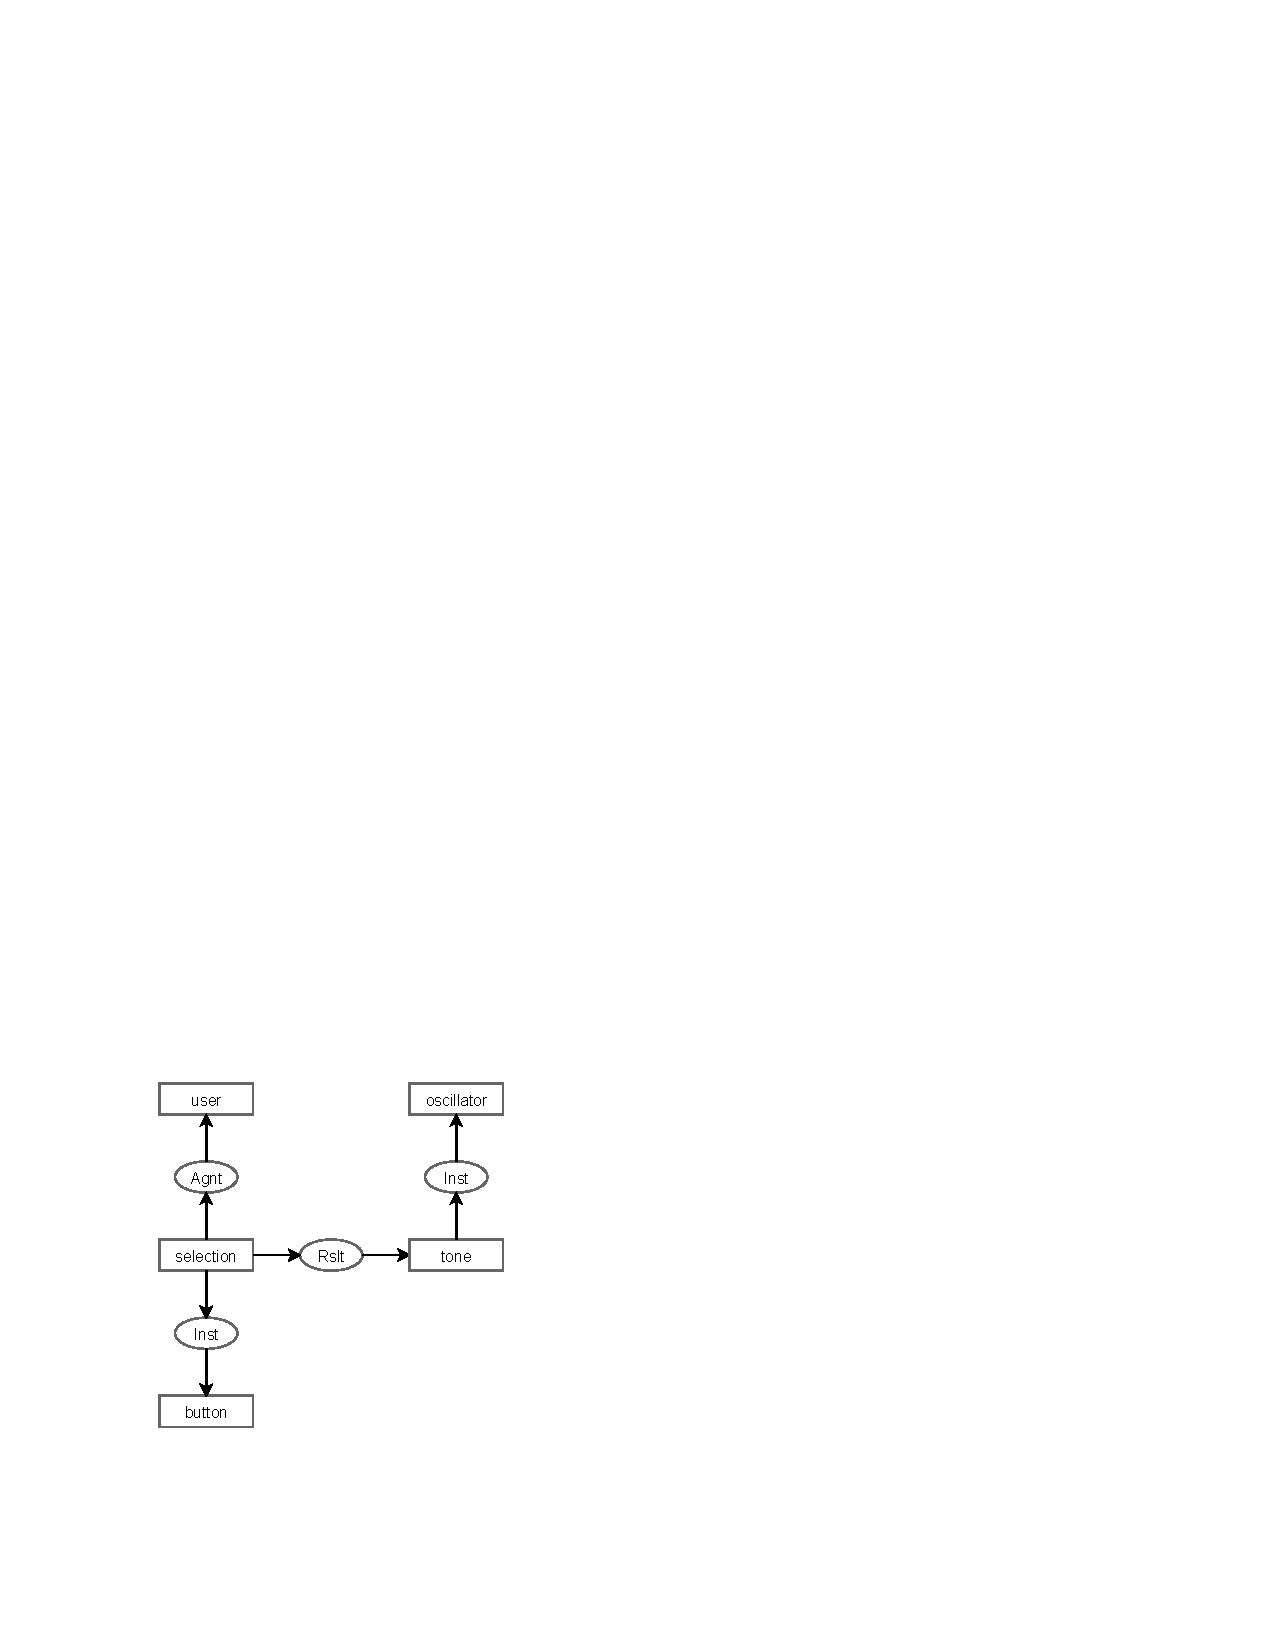
\includegraphics[scale=1]{./figures/oscillator.pdf}} \\
  \subfloat[~]{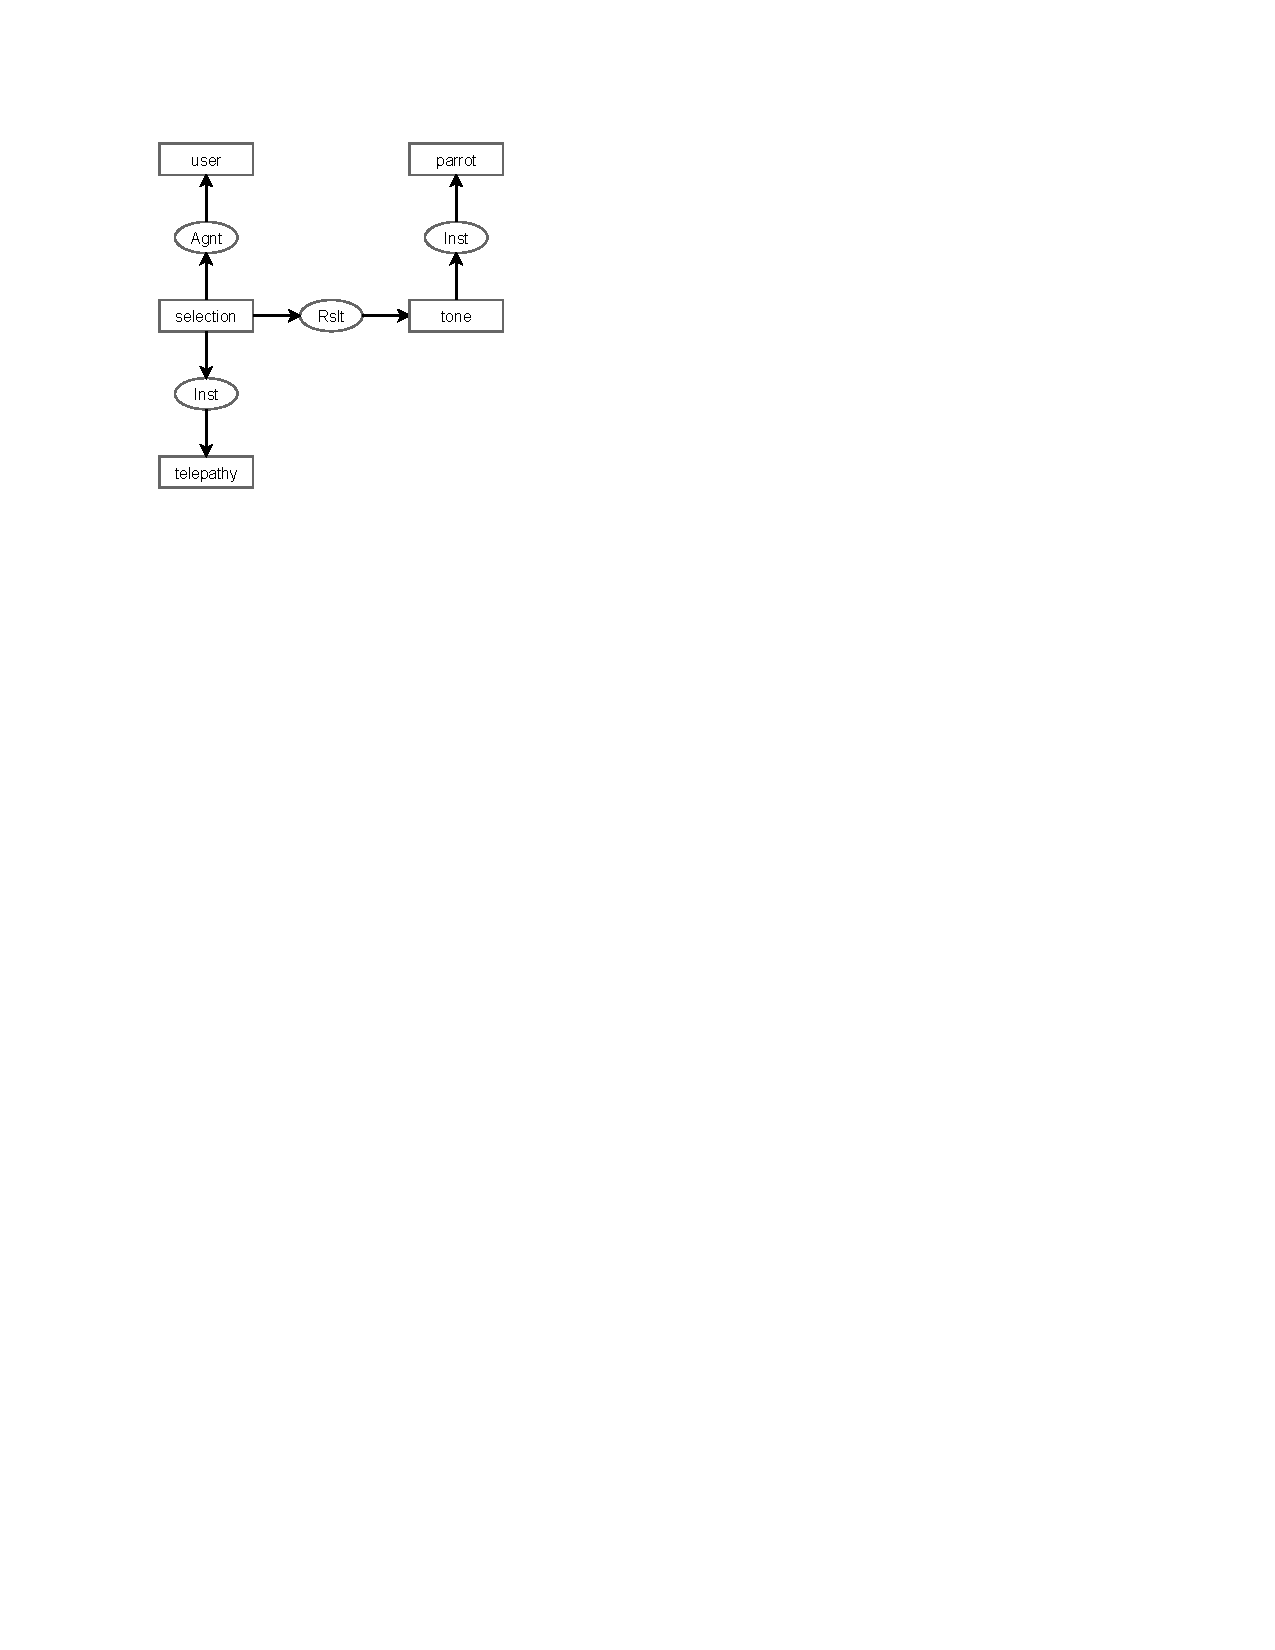
\includegraphics[scale=1]{./figures/parrot.pdf}} \\
  \subfloat[~]{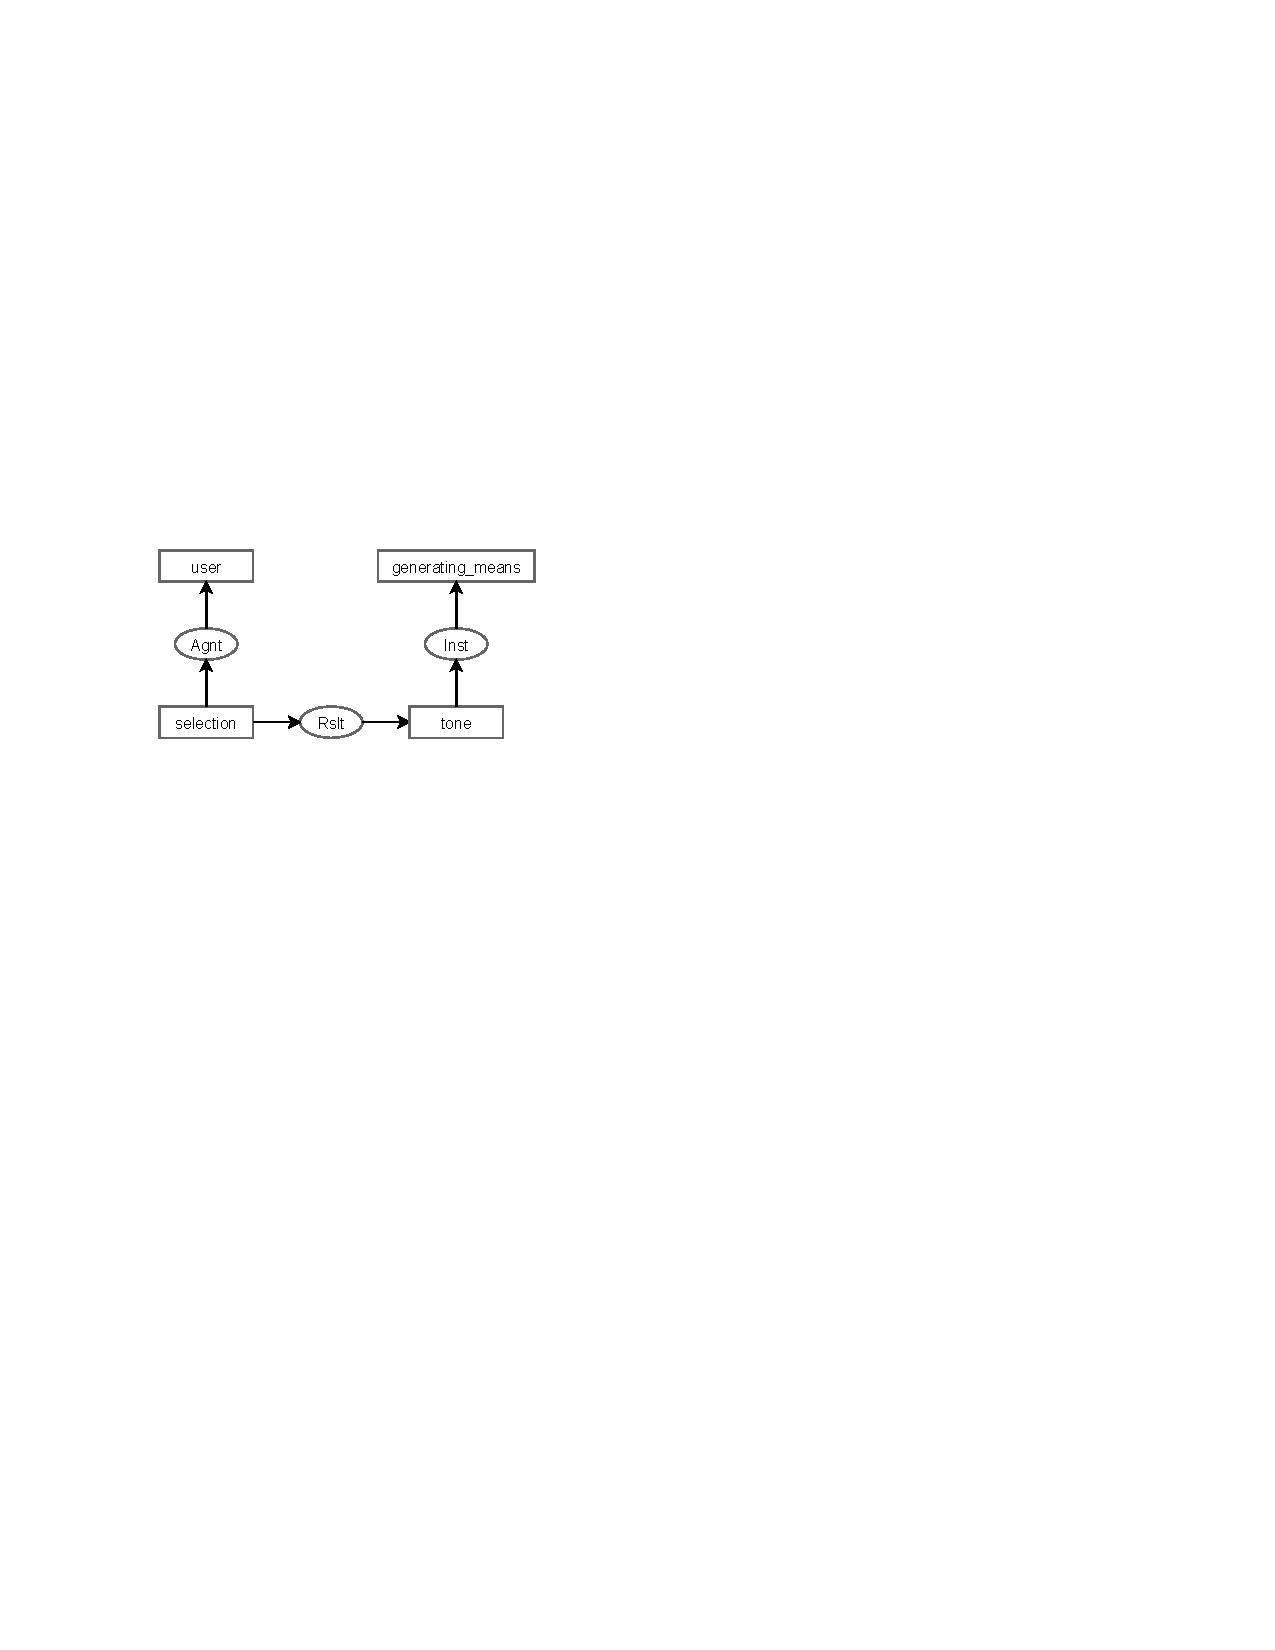
\includegraphics[scale=1]{./figures/leastgen.pdf}}
\caption{(a) 1st embodiment, (b) 2nd embodiment, (c) least generalization}
\label{fig:leastgen}
\end{figure}

The least generalization is shown in figure~\ref{fig:leastgen}(c). Roughly, this graph shows what is most common between the two embodiments (a) and (b) (i.e., ``the unifiable overlap'').\footnote{Here we have assumed that, in the ontology, parrot and oscillator are both kinds of ``generating means''.} That is, a user makes a selection and a tone is generated by some means. In the next section, we will see that the least generalization can be applied usefully when contemplating a broad claim.

\section{Claims}\label{sec:claims}

%\epigraph{Most of the fundamental ideas of science are essentially simple, and may, as a rule, be expressed in a language comprehensible to everyone.}{Albert Einstein}
\epigraph{You have to learn the rules of the game. And then you have to play better than anyone else.}{Albert Einstein}


%\epigraph{We've got no money, so we've got to think.}{Ernest Rutherford}.

A patent is a teaching to improve the prior art, and its mechanism for improvement is the {\em rule}. A rule teaches how to achieve a certain improvement for a given situation. The improvement of a preferred embodiment, for example, corresponds to a relatively specialized rule, while a claim corresponds to a more general rule.

Rules are native to conceptual graph theory, and require two graphs to define them: one for the initial situation (typically called the {\em Hypothesis} graph, $H$), and one for the improvement (typically called the {\em Conclusion} graph, $C$). A CG rule may apply to a specific embodiment, or a claim, or anything in between---depending on $H$ and $C$. Typically $H$ and $C$ for a claim will be more general than $H$ and $C$ for a specific embodiment.

A rule can be paraphrased as, ``whenever $H$ is true, $C$ can be added''---rules {\em add knowledge}~\footcite{Chein09}. Figure~\ref{fig:happycat} shows a simple CG rule, which can be paraphrased as ``if a cat is on a mat, it is a happy cat''.\footnote{The dashed line indicates that it is the same cat in both $H$ and $C$.}

\begin{figure}
\centering
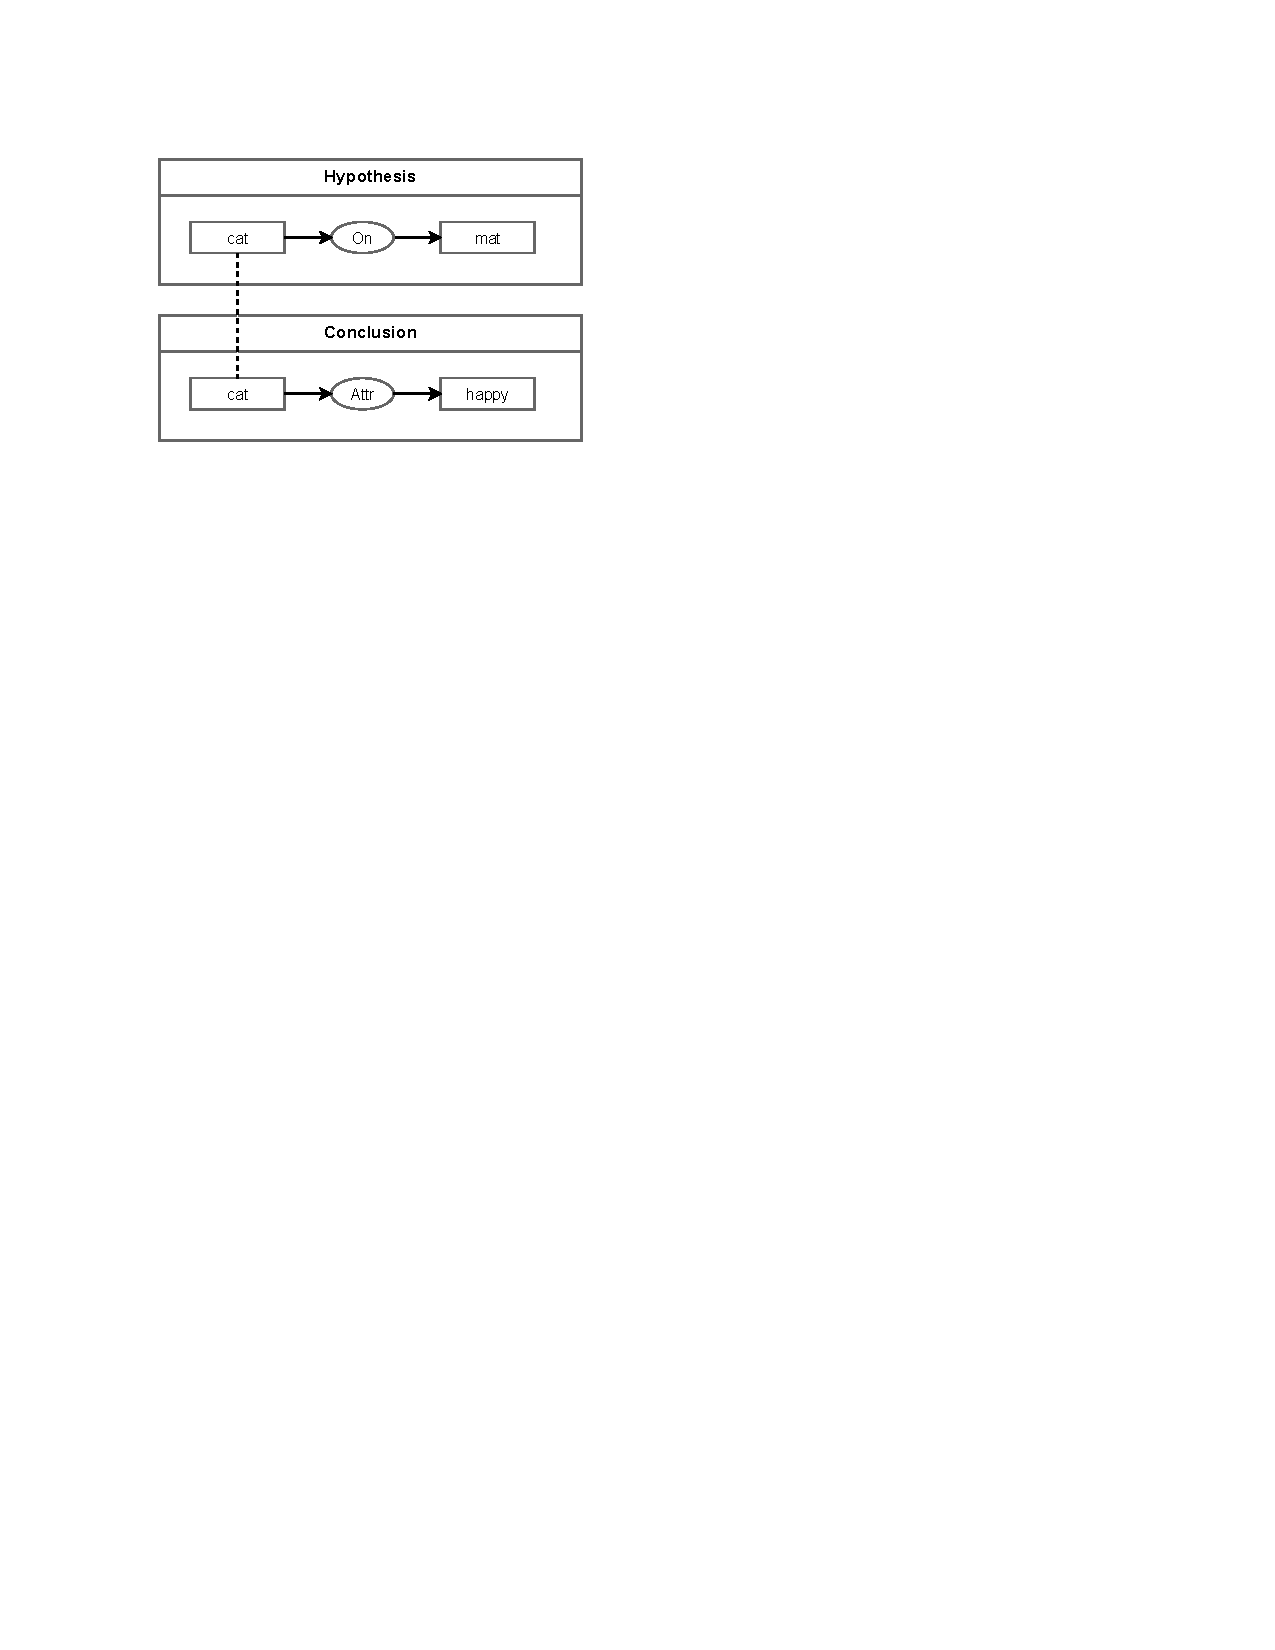
\includegraphics[scale=1]{./figures/happycat.pdf}
\caption{A simple rule}
\label{fig:happycat}
\end{figure}

For IACS, a rule is applied by projecting the hypothesis graph into the prior art; whenever the projection is successful (that is, whenever $H$ or any specialization of $H$ can be found), then the knowledge of the conclusion graph can be added. For example, according to figure~\ref{fig:happycat}, whenever we find a cat on a mat in the prior art, we can further add the knowledge that it is happy. In this sense, a rule is a mapping between the set of prior art and the set of possible embodiments. The domain, $\mathbb{D}$, of the mapping is every instance of prior art into which $H$ projects; the range, $\mathbb{R}$, is every element of $\mathbb{D}$ improved by $C$. Figure~\ref{fig:ruleclouds} illustrates the relationship.

\begin{figure}
\centering
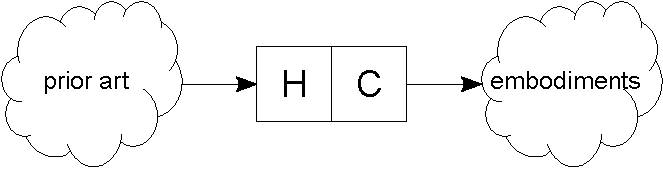
\includegraphics[scale=0.8]{./figures/ruleclouds.pdf}
\caption{Relationship between prior art graphs, hypothesis graph ($H$), conclusion graph ($C$), and embodiment graphs}
\label{fig:ruleclouds}
\end{figure}

Below we consider several applications of rules to synthesizing claims, beginning with the problem-solution statement; the workflow example in appendix~\ref{sec:workflow} further illustrates some of these approaches.

\subsection{Problem and Solution}

The problem-solution statement is an important approach to claim synthesis.\footnote{See, e.g., \cite{Pressman09}, \cite{Slusky07}, \url{http://en.wikipedia.org/wiki/Inventive_step_and_non-obviousness}.} In \cite{Slusky07}\footcite[Chapter~7]{Slusky07} the problem-related language is removed to leave a {\em pruned} statement, at which point we find a close parallel with CG rules.

The pruned problem-solution statement is a generalization, since it is not specialized (limited) by a description of the problem. However, the statement retains the {\em context} for the solution---that is, that part of the prior art to which the invention applies. Along with the context, the pruned statement provides an improvement. In CG terms, the context is the hypothesis graph $H$ and the improvement is the conclusion graph $C$.

For example, consider the following pruned problem-solution statement:\footcite[Chapter~7]{Slusky07}
%
\begin{quote}
\sout{The problem of nonuniform heating of} food \sout{is solved by} engendering relative motion between the food and the energy source.
\end{quote}
%
The corresponding hypothesis and conclusion graphs are shown in figure~\ref{fig:uwaveproblemsolution}. The hypothesis graph asserts an energy source and food. The conclusion graph asserts movement between the food and the source. Thus, this rule says whenever we find an energy source and food, the situation can be improved with movement between the food and the source.

\begin{figure}
\centering
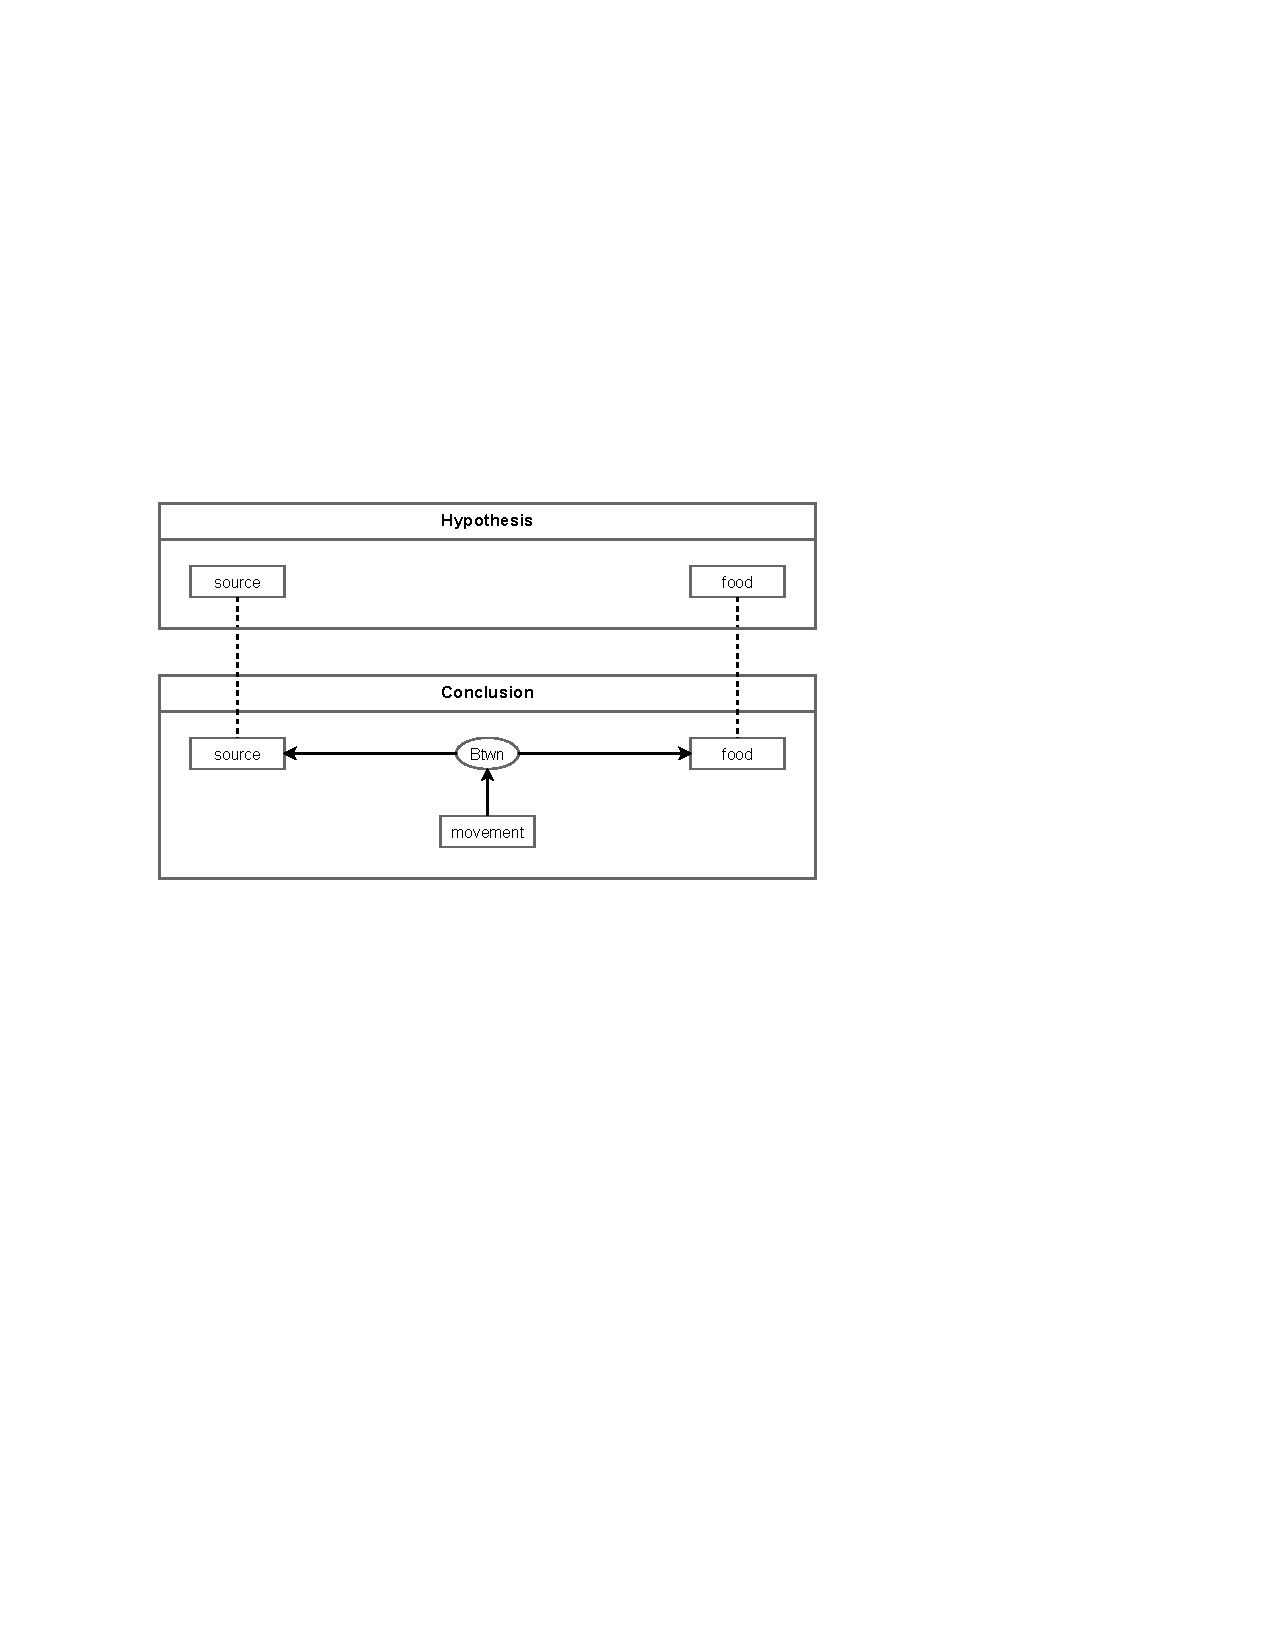
\includegraphics[scale=1]{./figures/uwaveprobsol.pdf}
\caption{Pruned problem-solution statement as a rule}
\label{fig:uwaveproblemsolution}
\end{figure}


\subsection{Inventive Departure}

The inventive departure, as viewed as the improvement to the prior art, is the conclusion graph $C$. For instance, in the microwave example above, the inventive departure is the movement between the energy source and food (as shown in the conclusion graph in figure~\ref{fig:uwaveproblemsolution}).

\subsection{First Claim}

The primary objective of claim synthesis is to find the broadest possible claim that doesn't read on the prior art. In CG terms, this corresponds to the rule for which: (a) the hypothesis graph projects into as much prior art as possible; and (b), the conclusion graph projects into as many potential infringers without projecting into said prior art. Or, said another way, a rule with a large domain $\mathbb{D}$, and a large range $\mathbb{R}$, for which there is no projection from $\mathbb{R}$ into $\mathbb{D}$.

In optimizing the rule, problems may occur with either $H$ or $C$. For example, the hypothesis of figure~\ref{fig:uwaveproblemsolution} projects on a rotisserie oven while the conclusion projects {\em on the same art}---thus invalidating the claim. Figure~\ref{fig:notrotisserie} shows a refinement where a cavity is added,\footnote{The cavity is the recipient (Rcpt) of the energy source, and is the location (Loc) of the food.} and thus avoids projection of $H$ into the prior art and saves the claim.

\begin{figure}
\centering
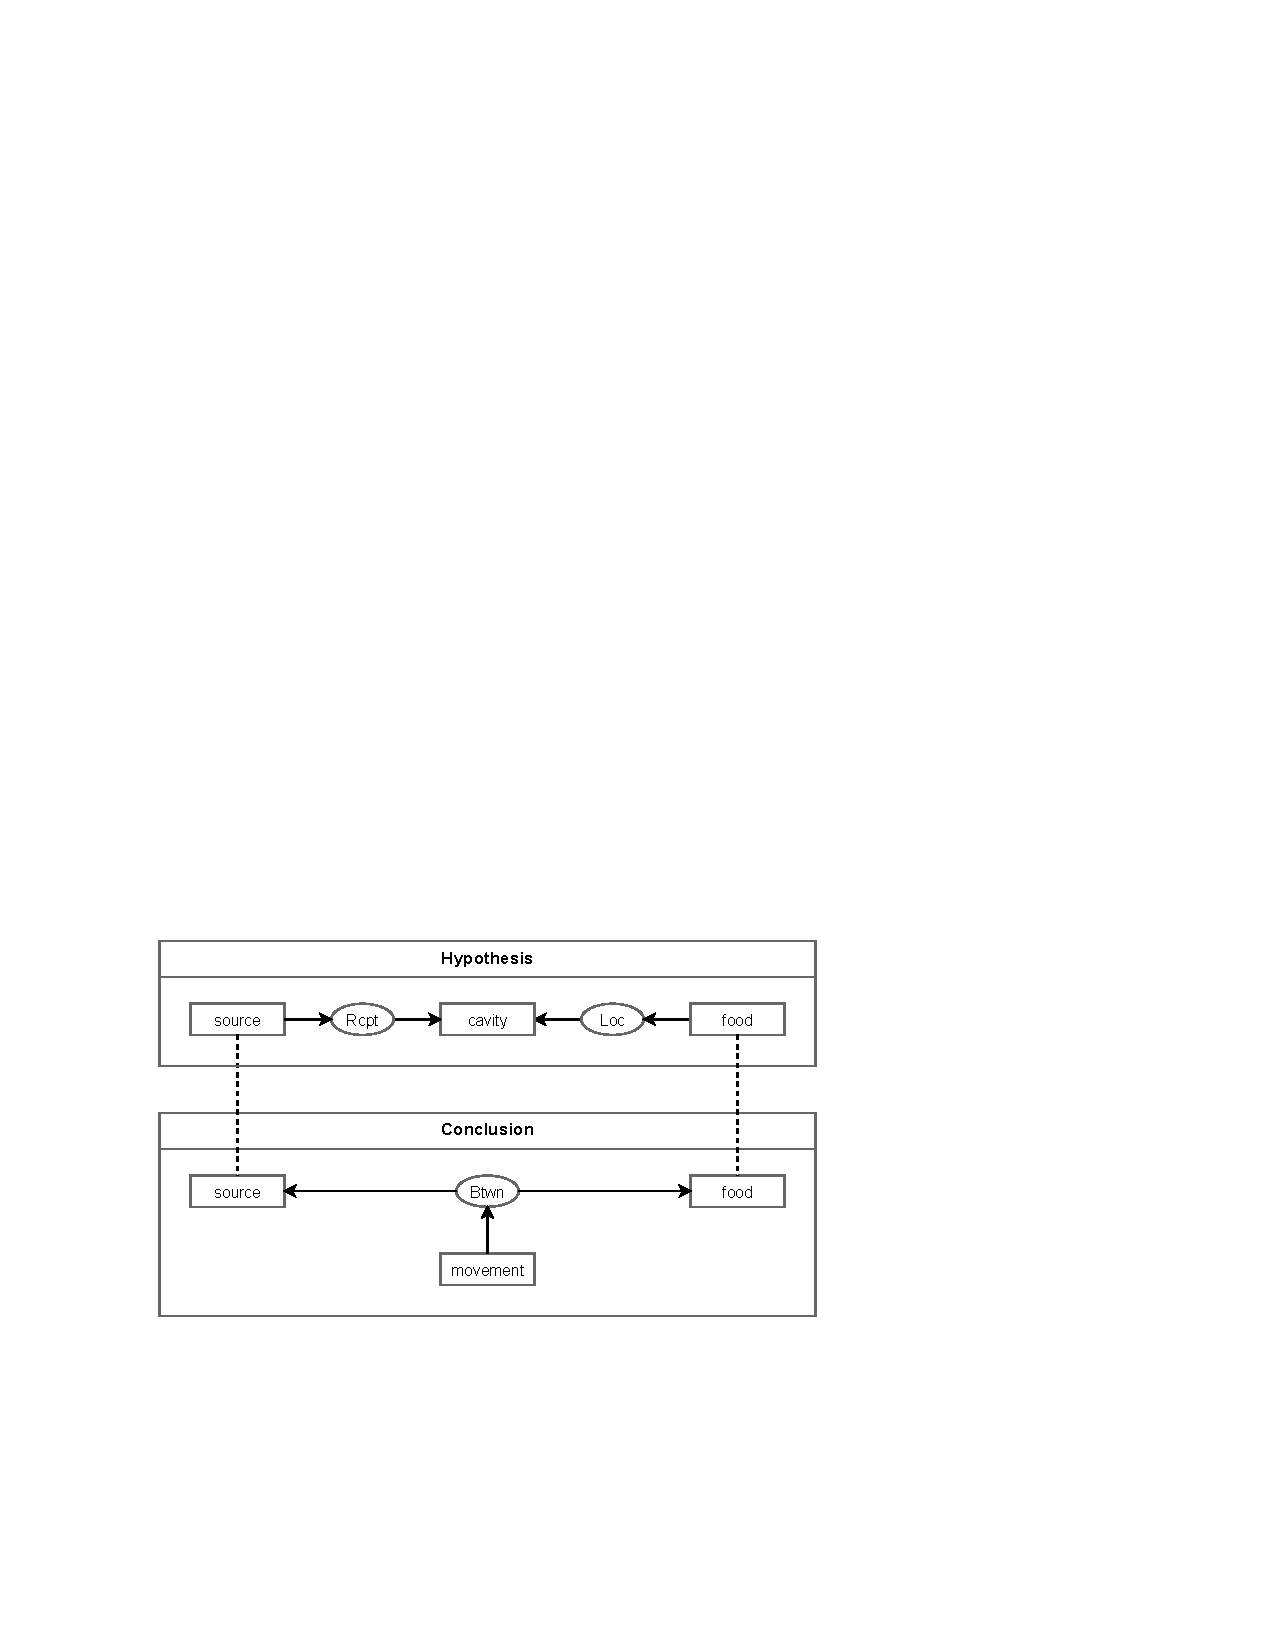
\includegraphics[scale=1]{./figures/notrotisserie.pdf}
\caption{Over-broad hypothesis}
\label{fig:notrotisserie}
\end{figure}

Within the constraints of the prior art, we want $H$ and $C$ to be as general as possible to capture as many potential infringers as the invention's essence will allow. Since a rule is simply two graphs, we can apply the generalization rules from section~\ref{sec:CGprimer}. However, if multiple embodiments are available (even far-fetched ``straw-man'' embodiments), we can apply the least generalization operation introduced in section~\ref{sec:leastgen} (see appendix~\ref{sec:workflow} for an example).

\subsection{Fallback Claims}

A fallback claim is often a specialization of a preceding claim. In CG terms this is straightforward as: claims are rules; rules are graphs; and, we know how to specialize graphs. Figure~\ref{fig:pencil} shows the idea of a chained rule---the hypothesis graph and conclusion graph \#1 claim a pencil that has a rod as one of its parts. Conclusion graph \#2 is chained to \#1, and has the additional specialization (restriction) that the rod is a graphite rod.

\begin{figure}
\centering
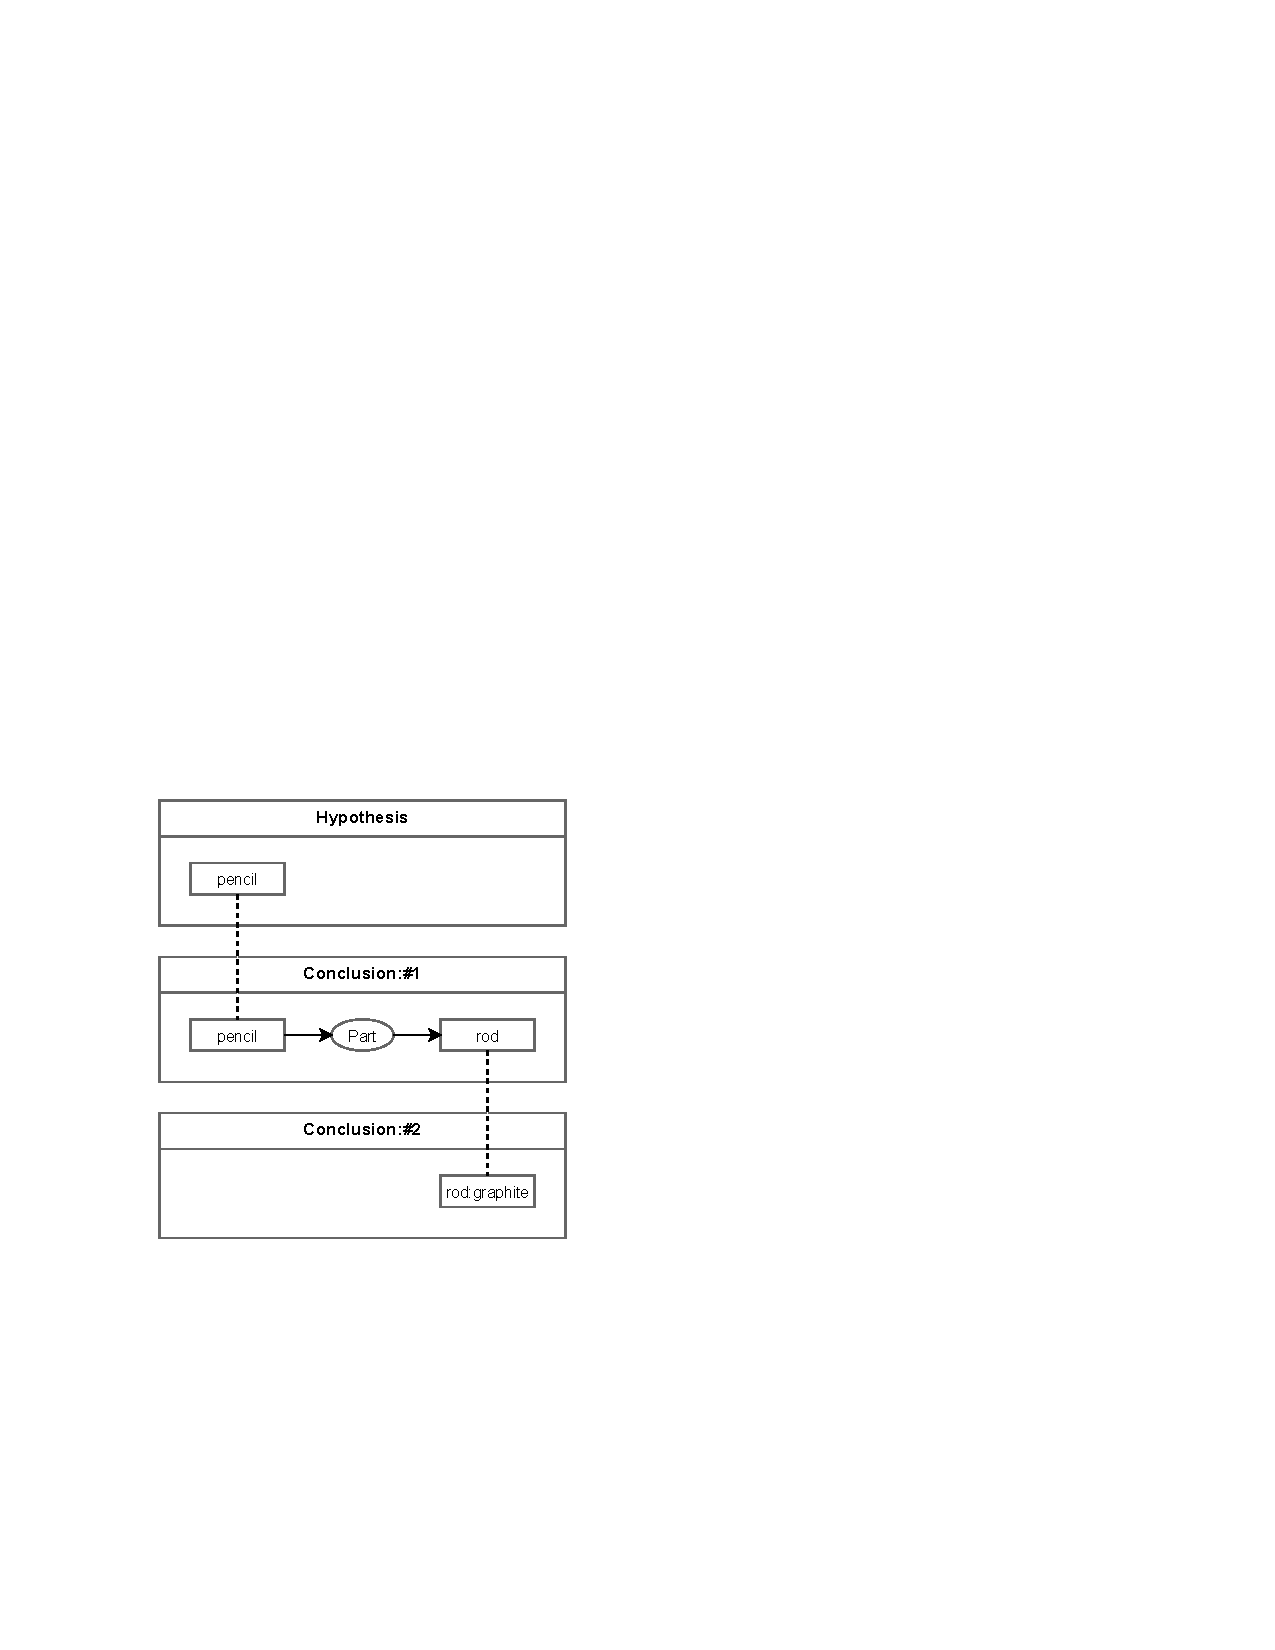
\includegraphics[scale=1]{./figures/pencilclaim.pdf}
\caption{A fallback claim using a chained rule}
\label{fig:pencil}
\end{figure}

\subsection{Definition Claims}

A definition claim can be similarly defined in CG terms. In the case shown in figure~\ref{fig:definition},\footcite[Chapter 10]{Slusky07} the significant differences from the fallback claim (figure~\ref{fig:pencil}) are that the specialization is via a graphical definition (rather than a restriction), and it is applied to the hypothesis (not the conclusion). In CG terms, hypothesis \#2 is known as a {\em nested graph}.

The rule in figure~\ref{fig:definition} improves a bimetallic switch (Hypothesis \#1) with a `doodad' (Conclusion). Hypothesis \#2 further defines bimetallic as two or more overlapping strips with nonequal coefficients of thermal expansion.

\begin{figure}
\centering
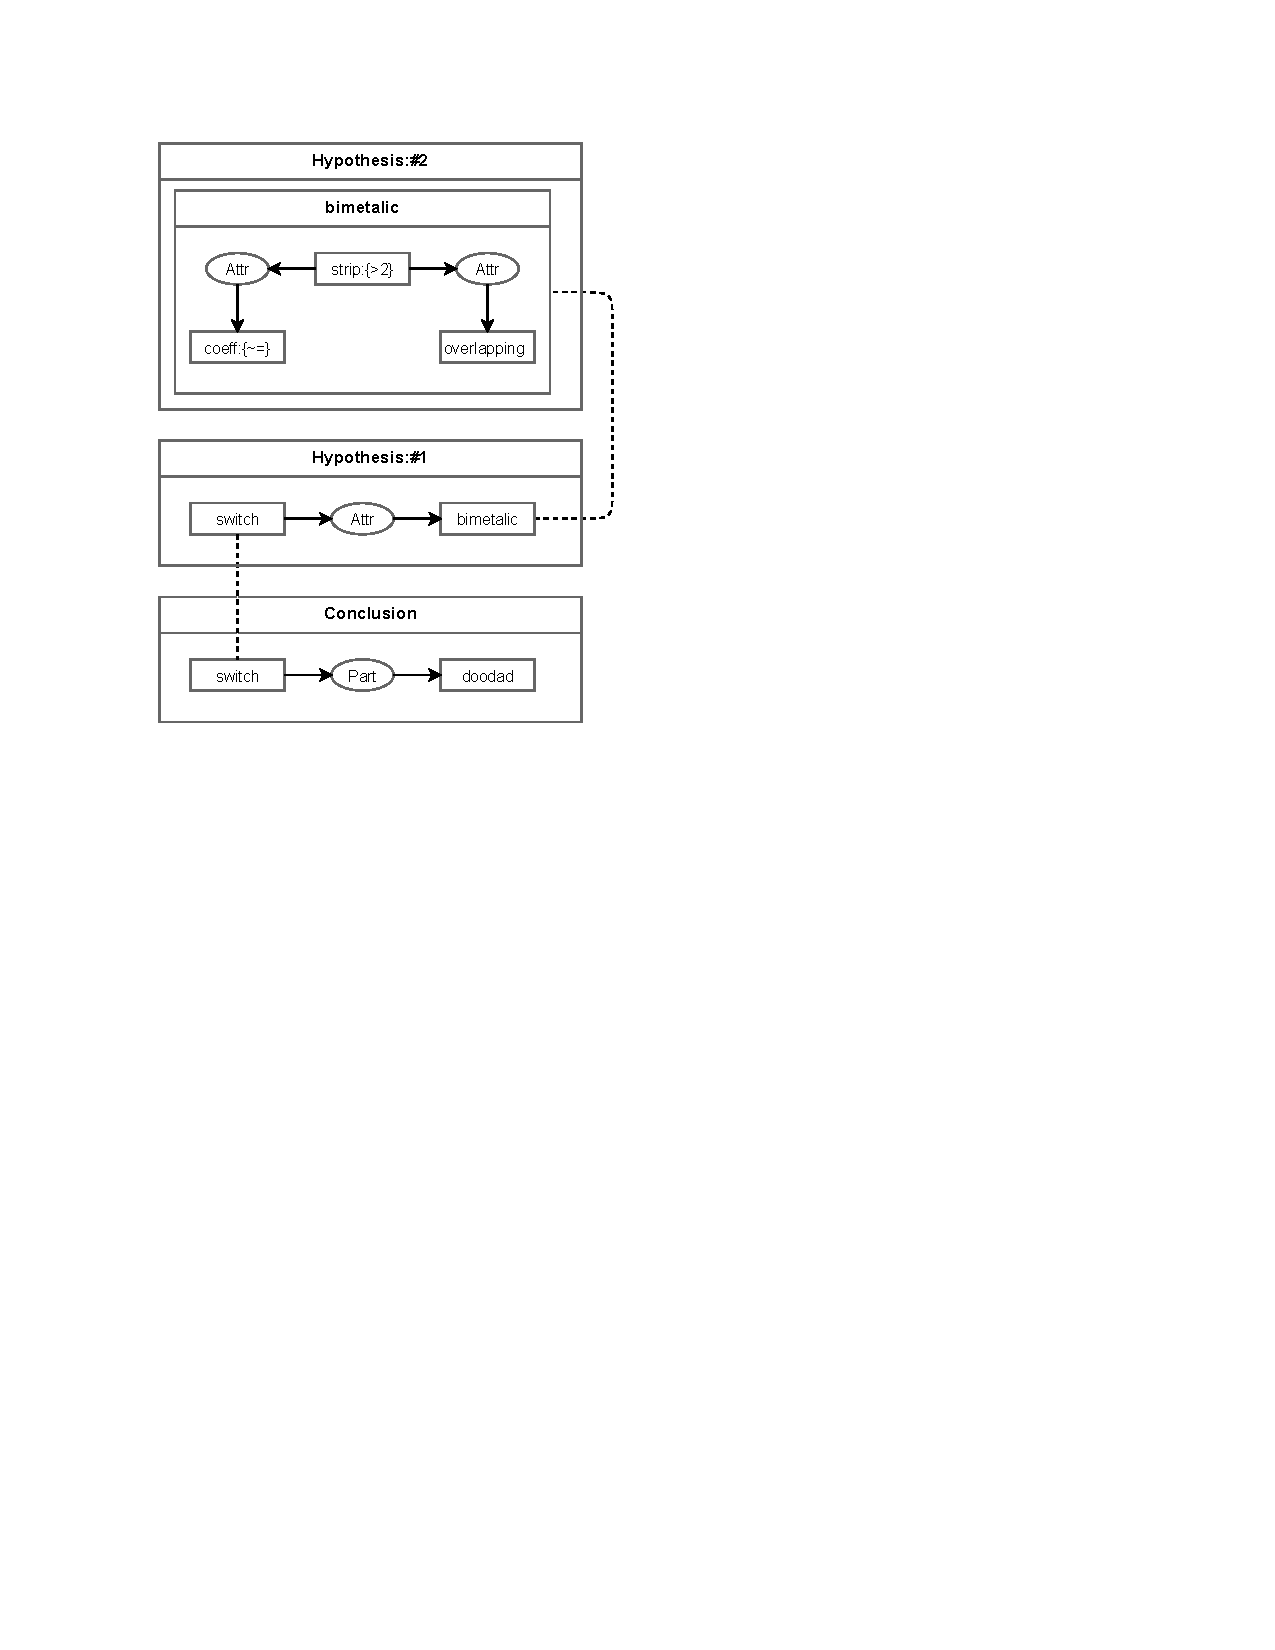
\includegraphics[scale=1]{./figures/switchdoodad.pdf}
\caption{Definition claim}
\label{fig:definition}
\end{figure}

\subsection{Independent Embodiment}

An independent embodiment is similar to the fallback and definition claim rules. Figure~\ref{fig:indembod}\footcite[Chapter 9]{Slusky07} shows a single hypothesis and two conclusions. The important difference is that the conclusions are not chained, but refer (independently) back to the hypothesis.

\begin{figure}
\centering
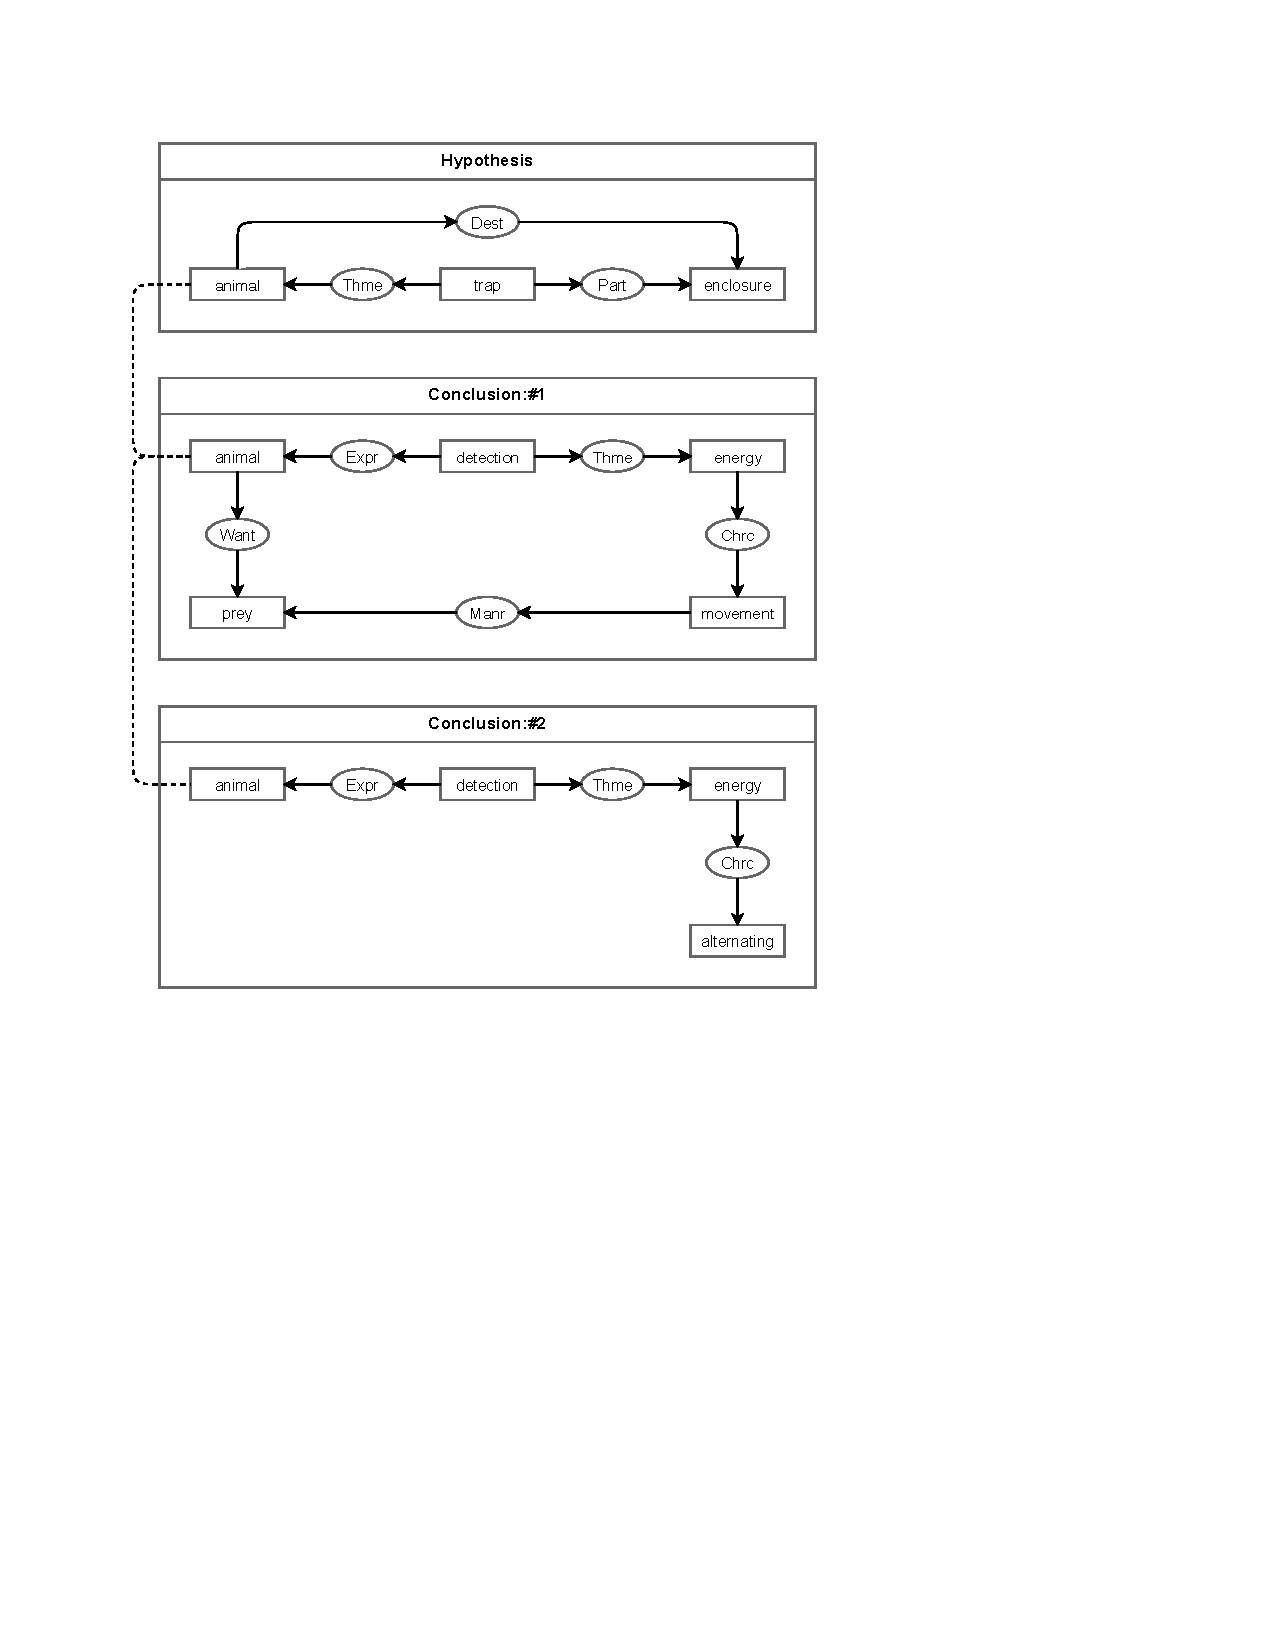
\includegraphics[scale=1]{./figures/indembodiment.pdf}
\caption{Independent embodiment}
\label{fig:indembod}
\end{figure}

Here the hypothesis graph asserts an animal trap (a trap with an animal theme) that has, as a part, an enclosure, and that the destination of the said animal is the enclosure. Conclusion \#1 is that the animal detects the energy (detection has an {\em experiencer}, an animal, and a theme, energy), furthermore, the energy has a movement characteristic of the prey of the animal. Conclusion \#2 is that the energy is simply alternating.

Having established a basis for the application of CG theory to IACS, we step back to consider the broader picture. The next section considers IACS as an engineering process, as enabled by CGs; the following section addresses enterprise IP portfolio management.

\section{Systems Engineering and Patent~Design}\label{sec:SystemsEngineering}

Engineering design has evolved to a point where the study of its own processes is itself a discipline, namely ``Systems Engineering''.\footnote{See, e.g., \cite{Sage00}.} Systems Engineering breaks the engineering process into three broad steps: (1) System Definition; (2) System Development; and, (3) System Deployment.

An example familiar to electronics engineers is circuit design, where (1) corresponds to determining the coefficients of a differential equation, (2) to determining a circuit to realize the differential equation, and (3) to building the circuit. Broadly stated, the process formalizes the idea that conceptual design (which is nimble and inexpensive) should precede implementation (which is neither).

Systems Engineering can be applied to patent drafting and facilitated with computer-aided CG technology:
\begin{enumerate}
\item[(1)]
{\bf Definition}: concepts and relations in the invention's ``world'' are committed to an ontology; the invention's embodiment(s) are represented as CGs; independent claims are derived via generalization (perhaps prompted by more advanced CG operations); dependent claims are derived by specializing independent claims (see appendix~\ref{sec:workflow} for an example).
\item[(2)]
{\bf Design}: invention facts (i.e., subgraphs\footnote{A subgraph is a small part of a larger encompassing graph.} from (1)) are rearranged to {\em define} the content of sections, paragraphs, figures and claims.
\item[(3)]
{\bf Deployment}: The text and figures of the patent application are drafted according to the CG definitions.
\end{enumerate}
%

It is instructive to examine more closely some interesting examples of Systems Engineering and their relationship to conceptual graphs and computer-aided design:

{\bf Design Flow}: the overall path of system definition, design and deployment is the sum of many smaller steps, which together are known as `design flow'. Design flow is critically important in complex engineering because, like a running relay, errors are prone at baton changes. Successful firms enforce strict controls on the flow of information---the use of particular software tools, data formats, design reviews, and so forth. Conceptual graphs can support the patent application design flow from initial disclosure, to the company review committee, to the inventor-attorney interview, to review, all the way to submission to the patent office.

{\bf Divide and Conquer}: a complex problem, properly considered, can often be broken down into a multitude of smaller problems. Indeed, engineers know that, in many practical cases, the smaller problems {\it per se} are not so difficult, but the management of their solution is critical. Thus, there must be an overarching plan (to break up a large problem), and the smaller problems must share a common language (so they can be reassembled). For patent design, Systems Engineering (via design flow) provides the required plan, and CG technology allows large problems to be subdivided.\footnote{We contend that the lack of a divide-and-conquer approach in patent application drafting largely limits (some combination of) the complexity, quality and speed of a draft to that an individual can handle. That is, it is difficult to have multiple workers, perhaps with different skills, all working together on the one design (a critical factor for the success of complex engineering projects).}

{\bf Design Rule Checking}: a Systems Engineering approach allows a design to be checked against rules for the process. In integrated circuit design this is known as Design Rule Checking (DRC). Design rules are common to all designs in a process. For example, in IC design, rules may constrain the minimum distance between elements in the physical layout. Similarly, there are also rules which apply to all patent applications---such as not including any aspect of the inventive concept in the background section; or, ensuring that every aspect of a claim has proper support in the specification. By representing embodiments, prior art, claims etc. with computer-readable conceptual graphs, automated DRC can be applied to patent drafts.

\section{Enterprise Applications}\label{sec:enterprise}
%\epigraph{In the middle of difficulty lies opportunity.}{Albert Einstein}
\epigraph{We can't solve problems by using the same kind of thinking we used when we created them.}{Albert Einstein}

Although the previous section refers tangentially to the application of CGs in large organizations, mostly we have considered the analysis of single inventions. However, an enterprise may deal with a very large number of new inventions---perhaps thousands---every year, which, in turn, introduces a new set of challenges and opportunities. Moreover, an enterprise likely has a large, existing, natural language (text-based) portfolio of disclosures, applications, and patents. Below we explore a selection of ways that CGs can help enterprises manage a large number of inventions, and better employ the latent knowledge of their IP portfolios.

Returning to the analogy of IC design, an enterprise garners significant benefit from enforcing the use of a common design environment.\footnote{E.g., see \url{http://www.cadence.com}.} This means that designers can efficiently collaborate on large projects, and that effort applied to design a circuit for one project can profitably be {\em reapplied} in another. Similarly, with patent design, inventions within the same domain often share similar approaches, ideas, concepts, and prior art. An enterprise can thus gain a similar advantage for its IP program from {\em design reuse} by requiring a common knowledge representation language. We contend that CGs are ideal, allowing results from the analysis of one invention to be applied to the analysis of others.

Two important elements for design reuse with CGs are searching (to locate and group similar inventions, for example) and ontology management. Searching is equivalent to a query applied to a CG invention database, and is achieved using projection. A search is defined by a graph, and any specializations of that graph in the database are returned as the result. For instance, in figure~\ref{fig:leastgen}, all three graphs would be returned for a query asking for selections that result in a `signal' --- but {\em only} if `tone' has been defined as type of `signal' in the ontology. Without proper ontology management there is no agreed set of terms on which a conceptual view of an enterprise's IP portfolio can be built. An ontology is similar to a library of models in a circuit design environment, and its concepts should be managed with a similar level of care. However, ontology management should not be seen as a burden, rather as the fair price of utility and precision.\footnote{Ontology management is also a critical issue for the semantic web.}

Enterprises not only need to analyze new inventions, but also a potentially large number of existing inventions---both their own, and those of their competition. Typically, these inventions are represented in natural language and the goals of the analyst are: (a) to employ the teaching of the enterprise's own invention; (b) to assign a value to a patent; or (c) to check a competitor's product for infringement. In each case the analyst must construct a conceptual view of the invention. But, without an effective way to record this view, the analysis is repeated many times, as either the analyst forgets, or others become interested in the invention. Conceptual graphs, on the other hand, allow a persistent record that can be peer-reviewed and evolve as required to better manage an enterprise's IP portfolio.

The key to reusing the teaching of an invention within an enterprise is the ability to search and group inventions according to their {\em conceptual} content. As discussed, natural language (particulary the language of patent documents) is not well suited to the task. It is very difficult, for example, for a computer to divine concepts from the text of a patent,\footnote{Also, in many cases, the same applies to engineers.} and so searching is typically limited to keywords. Conceptual graphs, alternatively, allow searching (via projection) for the {\em concepts} of interest. Of course, converting a large natural language IP portfolio to CGs is a significant task---but, as a matter of course, an analyst will construct a conceptual view {\em anyway}. Conceptual graphs offer a means to record this analysis, so that it can be read by computers, and used and improved by colleagues.

The value of a patent to an enterprise depends on its potential impact on competitors, both defensively (enabling the manufacture of an enterprise's product) and offensively (stopping or licensing a competitor's product). Typically, a value may be established by assessing a patent against a list of metrics, such as the age of the patent, the likelihood of infringement, the potential for a work-around, and so forth, with results recorded in a database. This approach, though, has fundamental shortcomings.

A patent's assessment depends, subjectively, on the conceptual views constructed by the analyst. While some subjectivity is unavoidable, a deeper problem is there is little or no record of the analyst's assumptions---the conceptual views of the prior art, the invention, and competitor's products. Such hidden assumptions mean the assessment is of limited value without the support of the analyst. A better approach is to use CGs to record what is known about the conceptual environment and to make any assumptions {\em explicit}. For example, say a CG rule is derived from a patent claim by a first analyst, and thus represents the analyst's conceptual view of the claim. Then, this view is subject to review by peers, and can also be applied by a computer. A CG representation of a competitor's product may be added to the database, and a computer can automatically determine, say, whether the product falls within the domain of the rule (i.e., whether the rule's hypothesis projects into the product).\footnote{Of course, the product does not infringe unless a projection of the rule's conclusion graph can also be found in the product---but, even if this not known, the analyst can easily use graphical techniques to mark assumptions as such. For example, by enclosing an assumed subgraph in a nested graph with an appropriate label.}

Not only is the evaluation of metrics subjective, but it may also become erroneous as competitors release new products, or new prior art becomes apparent. The enterprise is thus faced with the onerous task of maintaining its database, with analysts revisiting patents on a regular basis. This process of reassessing known inventions is extremely inefficient, given that {\em the inventions themselves have not changed}. A better approach is to properly construct a conceptual, computer-readable view of an invention {\em once} with CGs, and automate evaluations against prior art and new products as they come to hand.\footnote{A topic for future investigation is to what degree patent evaluation metrics can be determined by computer.}

The core problem, perhaps largely unrecognized, is that enterprises have few means---beyond natural language---to properly {\em represent} the knowledge in their portfolios. The tasks of evaluating, applying, and generally managing a portfolio rest critically with the familiarity of individual attorneys and engineers with the patents in their respective realms. For an enterprise, such a system is fragile (given that employees are ultimately transient) and may not be scalable (for a large and increasing IP portfolio in a rapidly changing world).

\section{Conclusion}\label{sec:conclusion}

\epigraph{Innovation is not the product of logical thought, although the result is tied to logical structure.}{Albert Einstein}

Conceptual graphs fit IACS like a glove, as summarized in table~\ref{tab:ideas} in the appendix. Conceptual graphs provide a common, expressive and logical language for attorneys, engineers and computers. The important notions of IACS have direct counterparts in CGs---inventions as a concept, the problem-solution statement, generalization and specialization, and claims all have natural and native representations in conceptual graph theory. As a machine readable language, CGs are thus an ideal basis to develop powerful computer tools (similar to those used by engineers and scientists) to assist with the logical structure of IACS.

On the other hand, interpreting natural language is a very difficult (largely unsolved) problem for computers. Natural language is similarly difficult for logical analysis---lacking the power, versatility, and simplicity of abstract mathematical language. If a key to a successful IACS process is harmonizing the {\em conceptual} views of the inventor and attorney, then we contend those views are better communicated with conceptual graphs---and not by continually construing and rendering natural language.

Conceptual graphs facilitate the {\em engineering} of patent applications, and, as such, are useful for managing enterprise-level IP portfolios.  By employing CGs for IACS, inventors and patent attorneys can thoroughly and systematically capture the essence of inventions and accurately synthesize claims. We believe that this approach will lead to higher-quality patents, delivered more efficiently, and with more benefit to the assignee.

\bibliography{./whitepaper}
\bibliographystyle{jurabib}

\newpage

\appendix

\section{Example Workflow}\label{sec:workflow}

Below we consider a simple example to show how to proceed, sequentially, from an embodiment to a claim.

\setlength{\parindent}{0pt}
\rule{\textwidth}{1pt}
First we draw an embodiment. The graph below is a specialization of figure~\ref{fig:cgPaEmbExample}(b), with a cubic cavity, and a 2 kilowatt magnetron. The embodied invention is the rotation of the food (`rotation' has theme `food' and effector `turntable').
\setlength{\parindent}{\mylength}

\begin{center} 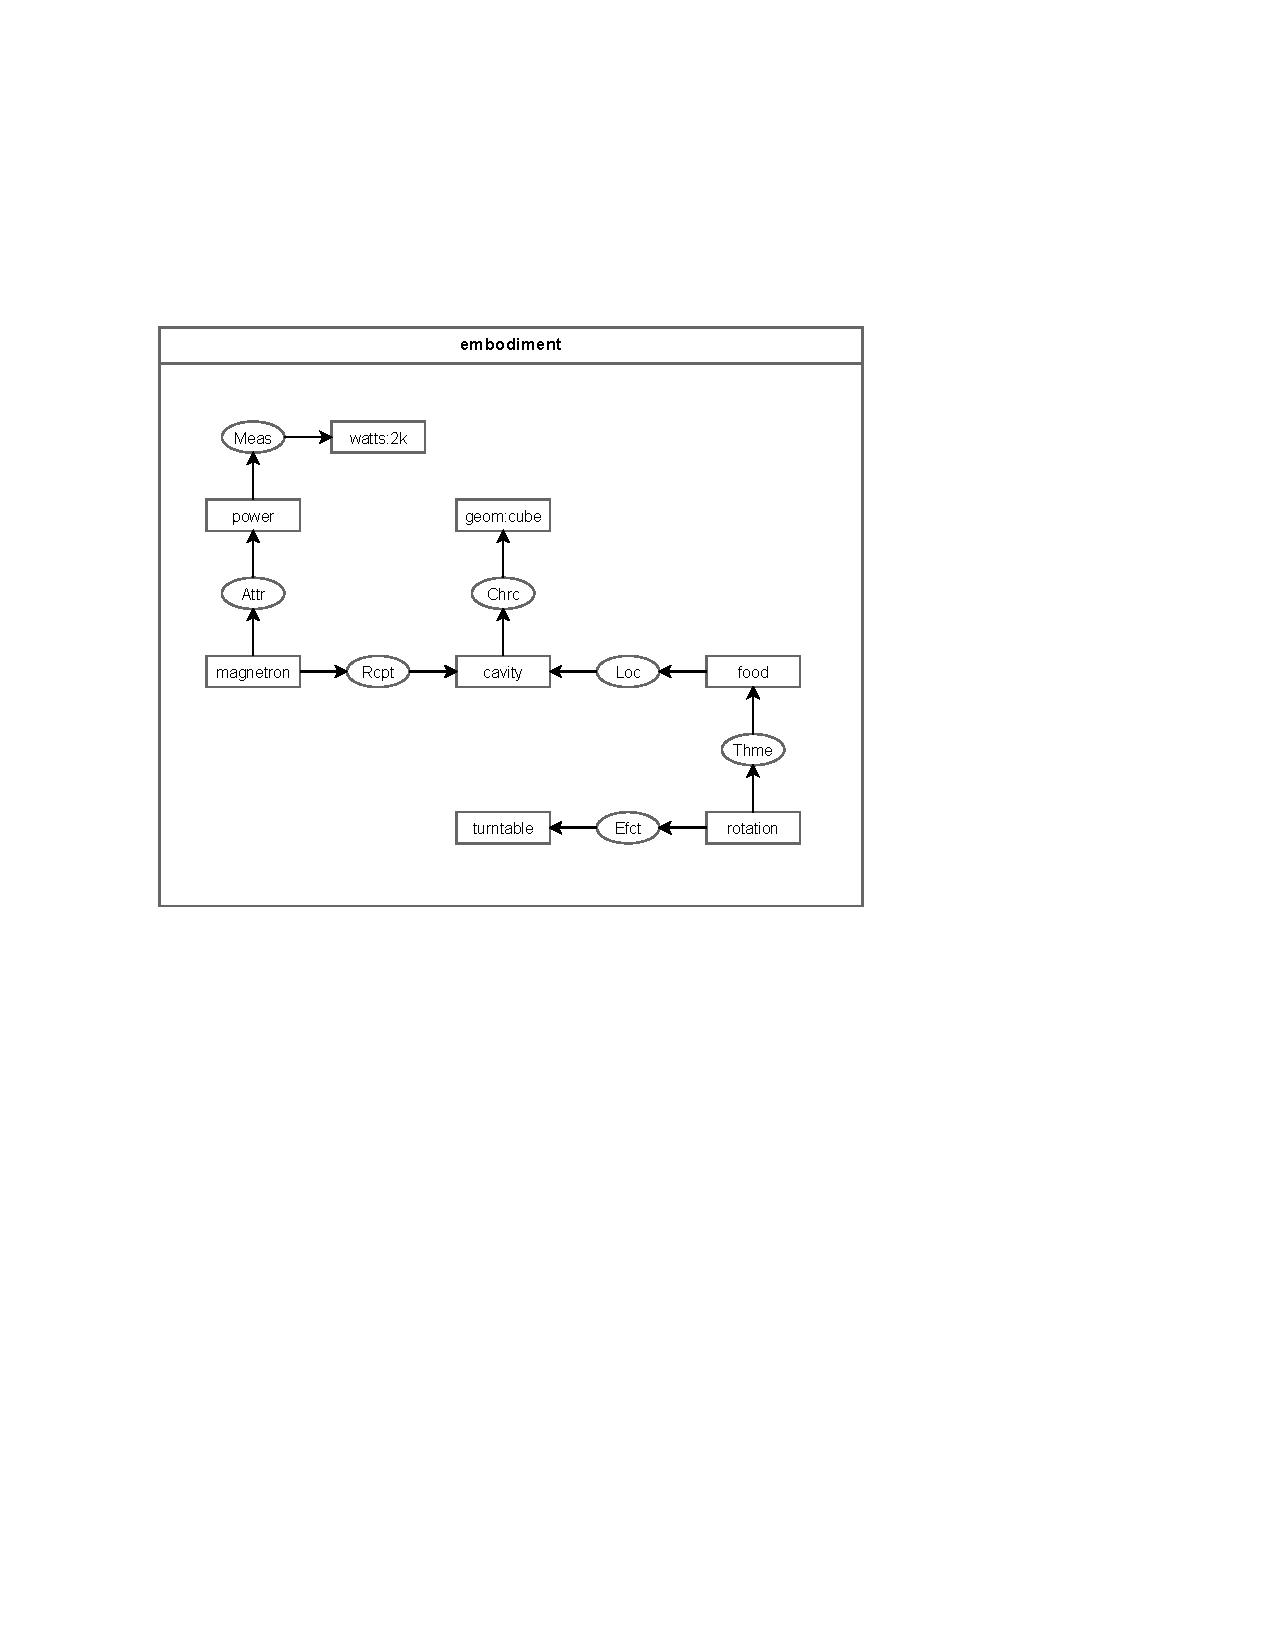
\includegraphics[width=0.70\textwidth]{./figures/wf_emb1.pdf} \end{center}

\setlength{\parindent}{0pt}
\rule{\textwidth}{1pt}
Next, we consider prior art---in the case below, a conventional oven (where a `cavity' is the location of `food' and the recipient of an energy `source'.). Note that `magnetron' (in the embodiment above) is a type of `source' (in the prior art below). We may write this as magnetron$<$source.
\setlength{\parindent}{\mylength}

\begin{center} 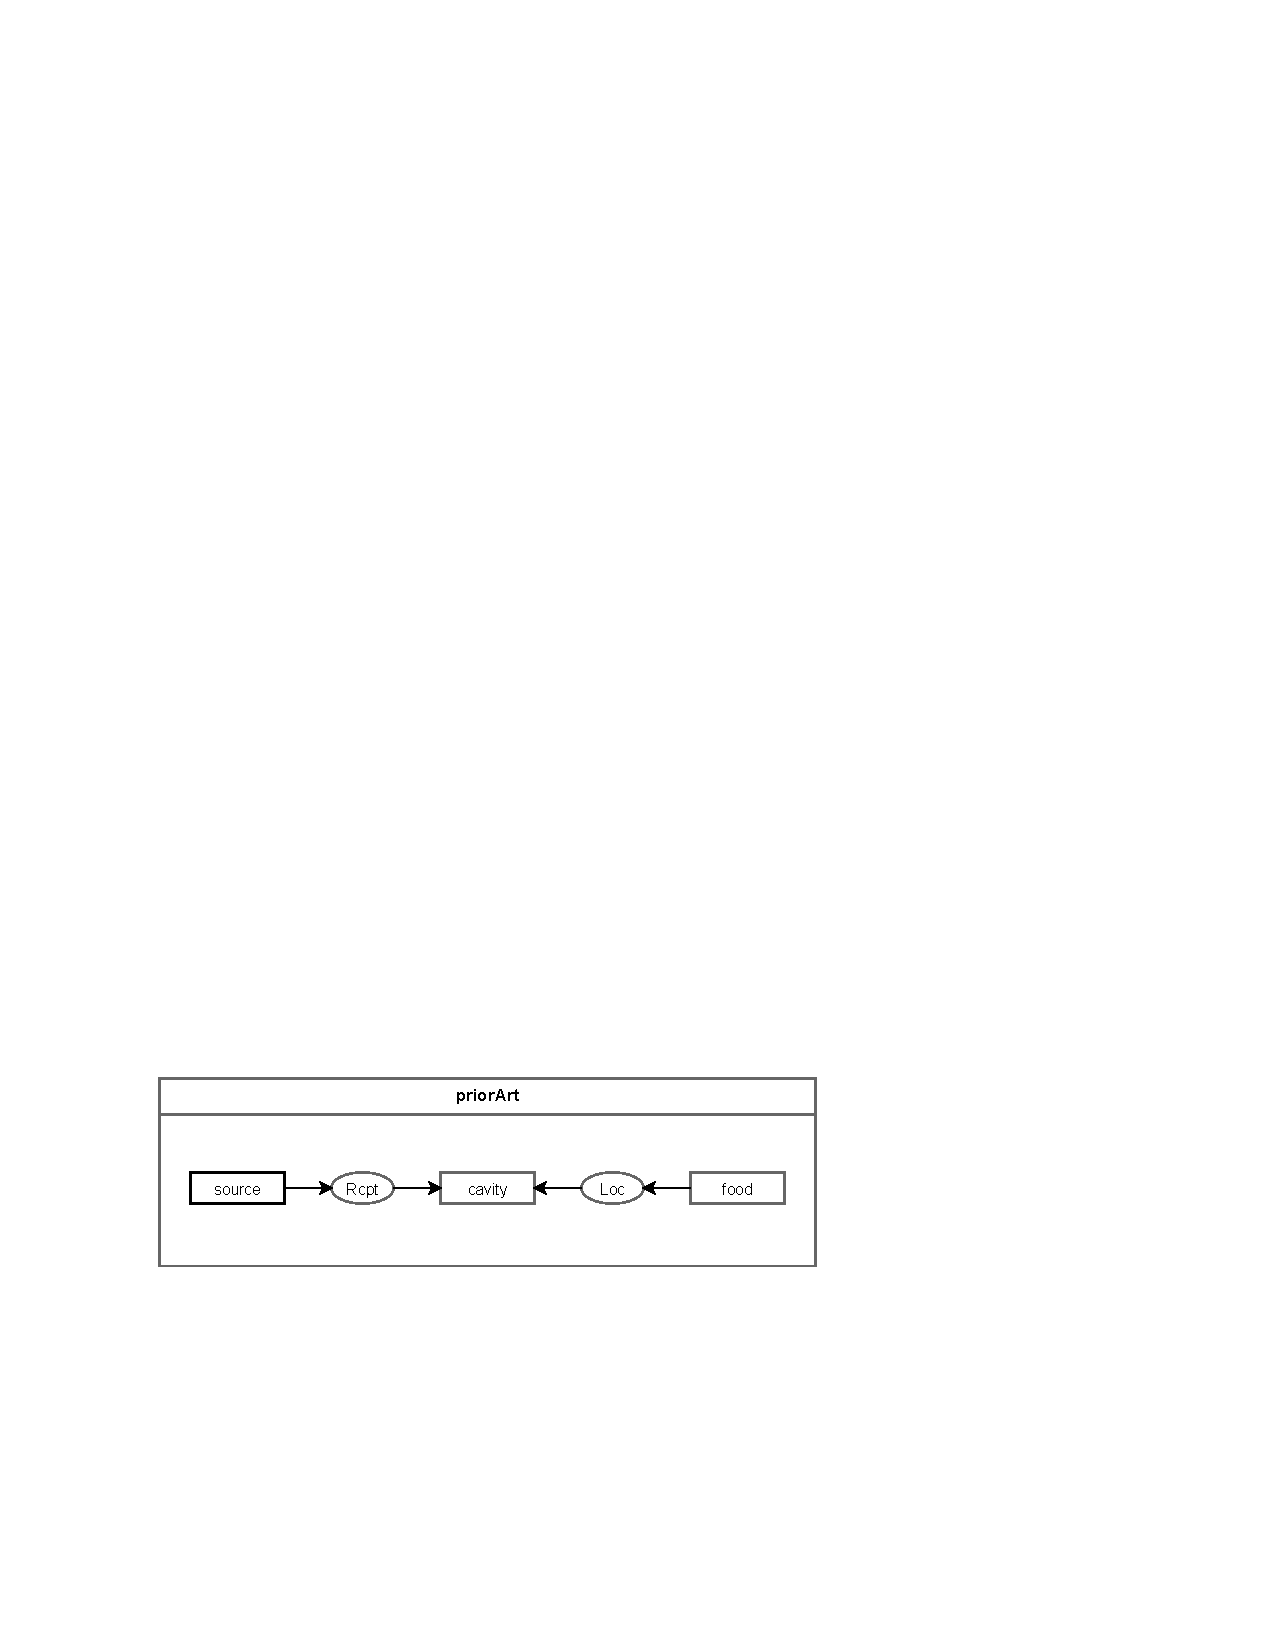
\includegraphics[width=0.70\textwidth]{./figures/wf_pa1.pdf} \end{center}

\setlength{\parindent}{0pt}
\rule{\textwidth}{1pt}
The prior art reads-on a portion of the embodiment. For conceptual graphs, reads-on is equivalent to projection. A first graph projects into a second if it (or any specialization) can be found in the second graph (see section~\ref{sec:inference}). Below, the projection of the prior art into the embodiment is highlighted; the highlighted subgraph indicates the part of the embodiment that the prior art reads-on. The parts of the embodiment that are not highlighted cannot be found in the prior art (or any specialization); however, not all are part of the inventive departure.
\setlength{\parindent}{\mylength}

\begin{center} 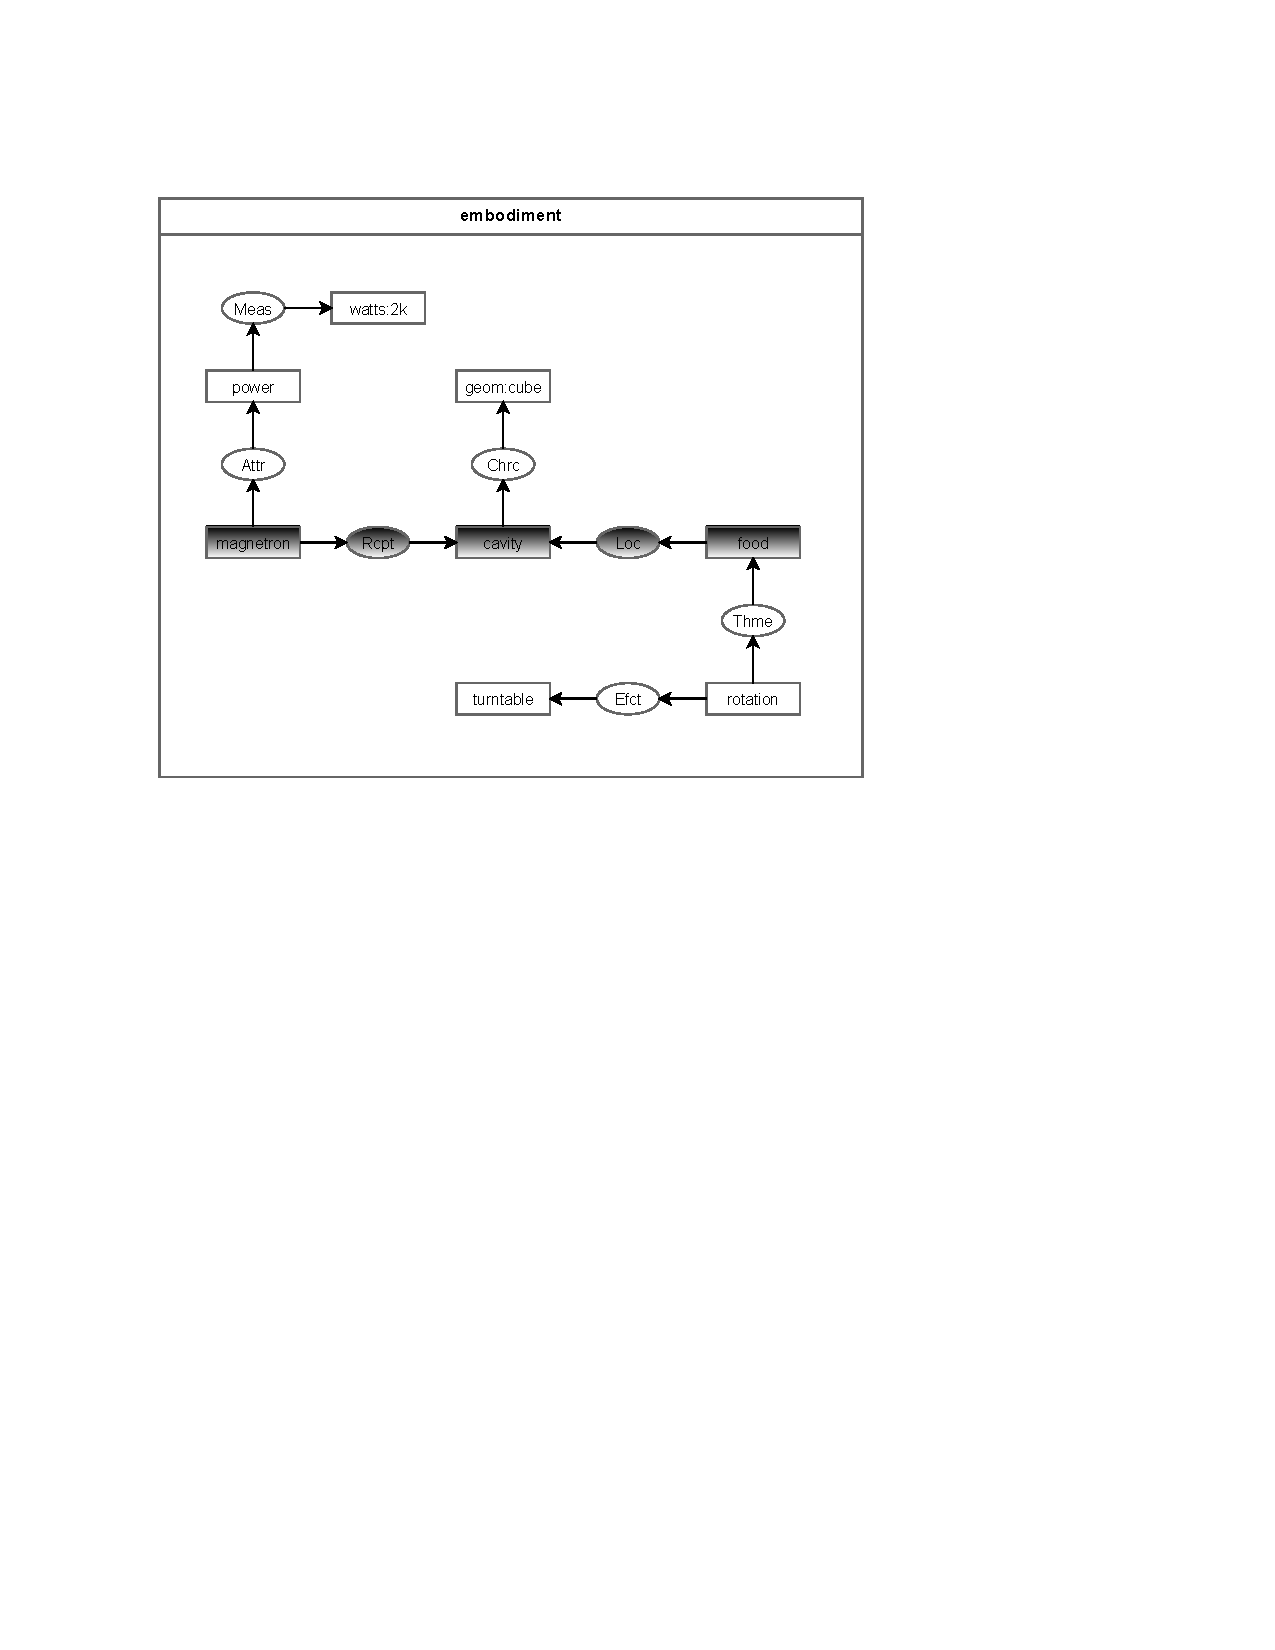
\includegraphics[width=0.70\textwidth]{./figures/wf_emb2.pdf} \end{center}

\setlength{\parindent}{0pt}
\rule{\textwidth}{1pt}
Guided by the highlighting in the embodiment, we make additions to the prior art. We assert that cubic cavities are known, as are 2 kW magnetrons.
\setlength{\parindent}{\mylength}

\begin{center} 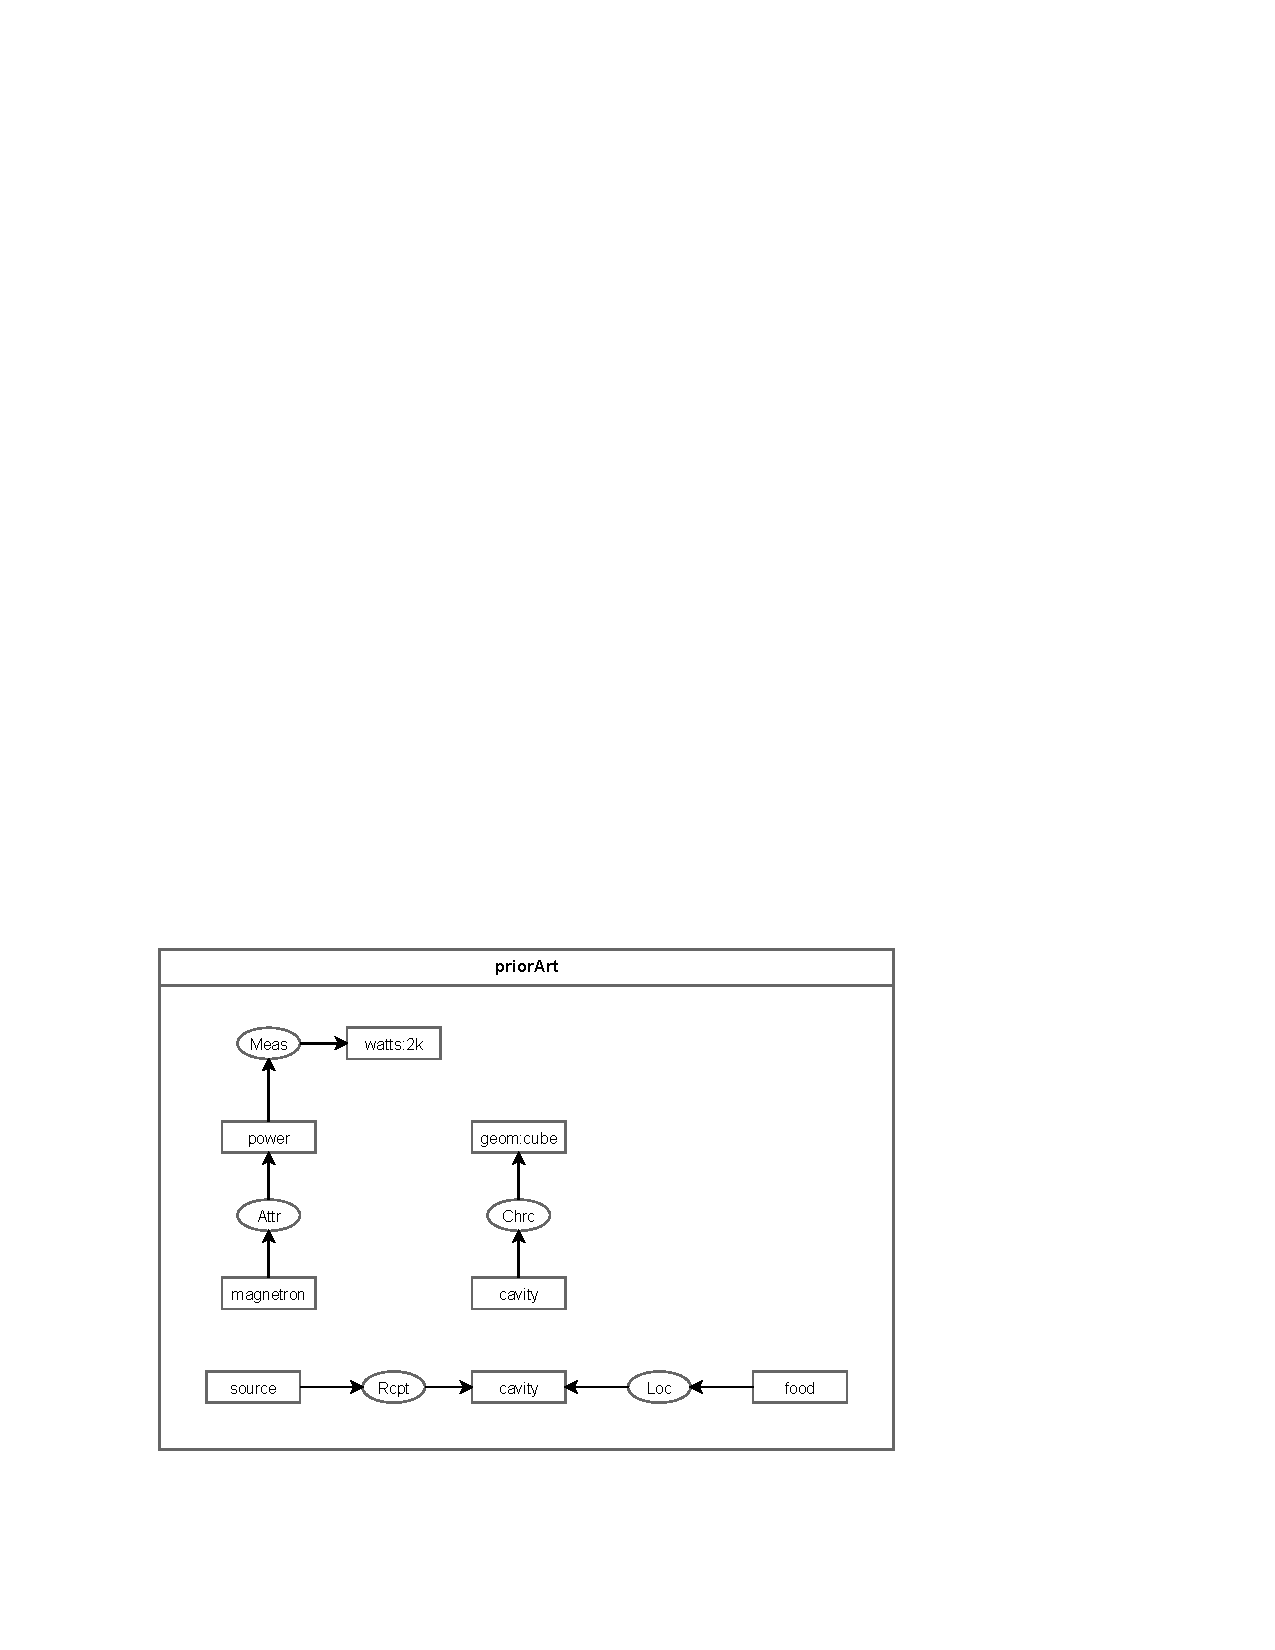
\includegraphics[width=0.70\textwidth]{./figures/wf_pa2.pdf} \end{center}

\setlength{\parindent}{0pt}
\rule{\textwidth}{1pt}
With the new prior art included, only the inventive part of the embodiment remains un-highlighted.
\setlength{\parindent}{\mylength}

\begin{center} 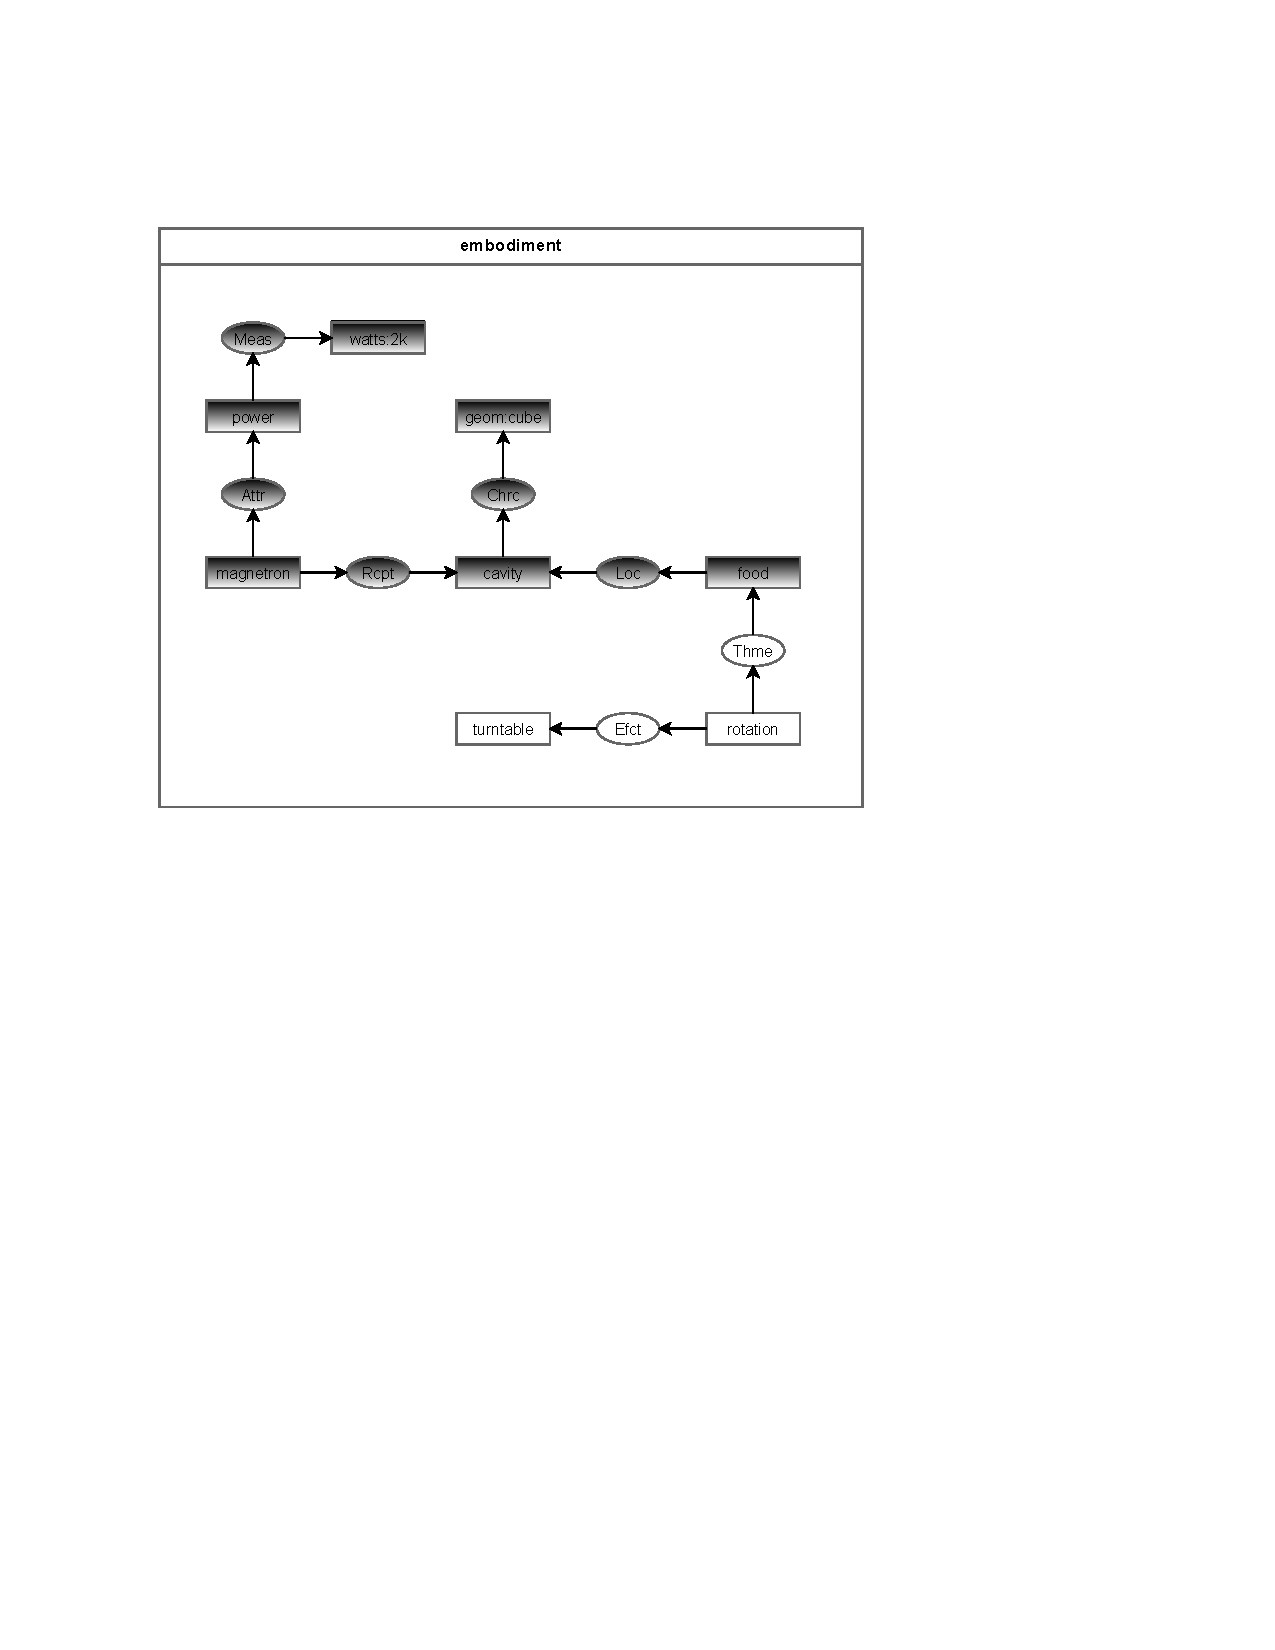
\includegraphics[width=0.70\textwidth]{./figures/wf_emb3.pdf} \end{center}

\setlength{\parindent}{0pt}
\rule{\textwidth}{1pt}
Having isolated the inventive departure we make a first attempt at a claim rule. Applying the principle ``pack only what you need'', we consider the minimum requirements for the hypothesis graph, $H$. Recalling that $H$ projects into the prior art (all prior art, not just what we have drawn), we must include enough to give the inventive step its proper context. Here we have chosen `source' and `food'---that is, we will apply the inventive step whenever we find these two concepts in the prior art. The inventive step is to rotate the food on a turntable, as shown in the conclusion graph, $C$.
\setlength{\parindent}{\mylength}

\begin{center} 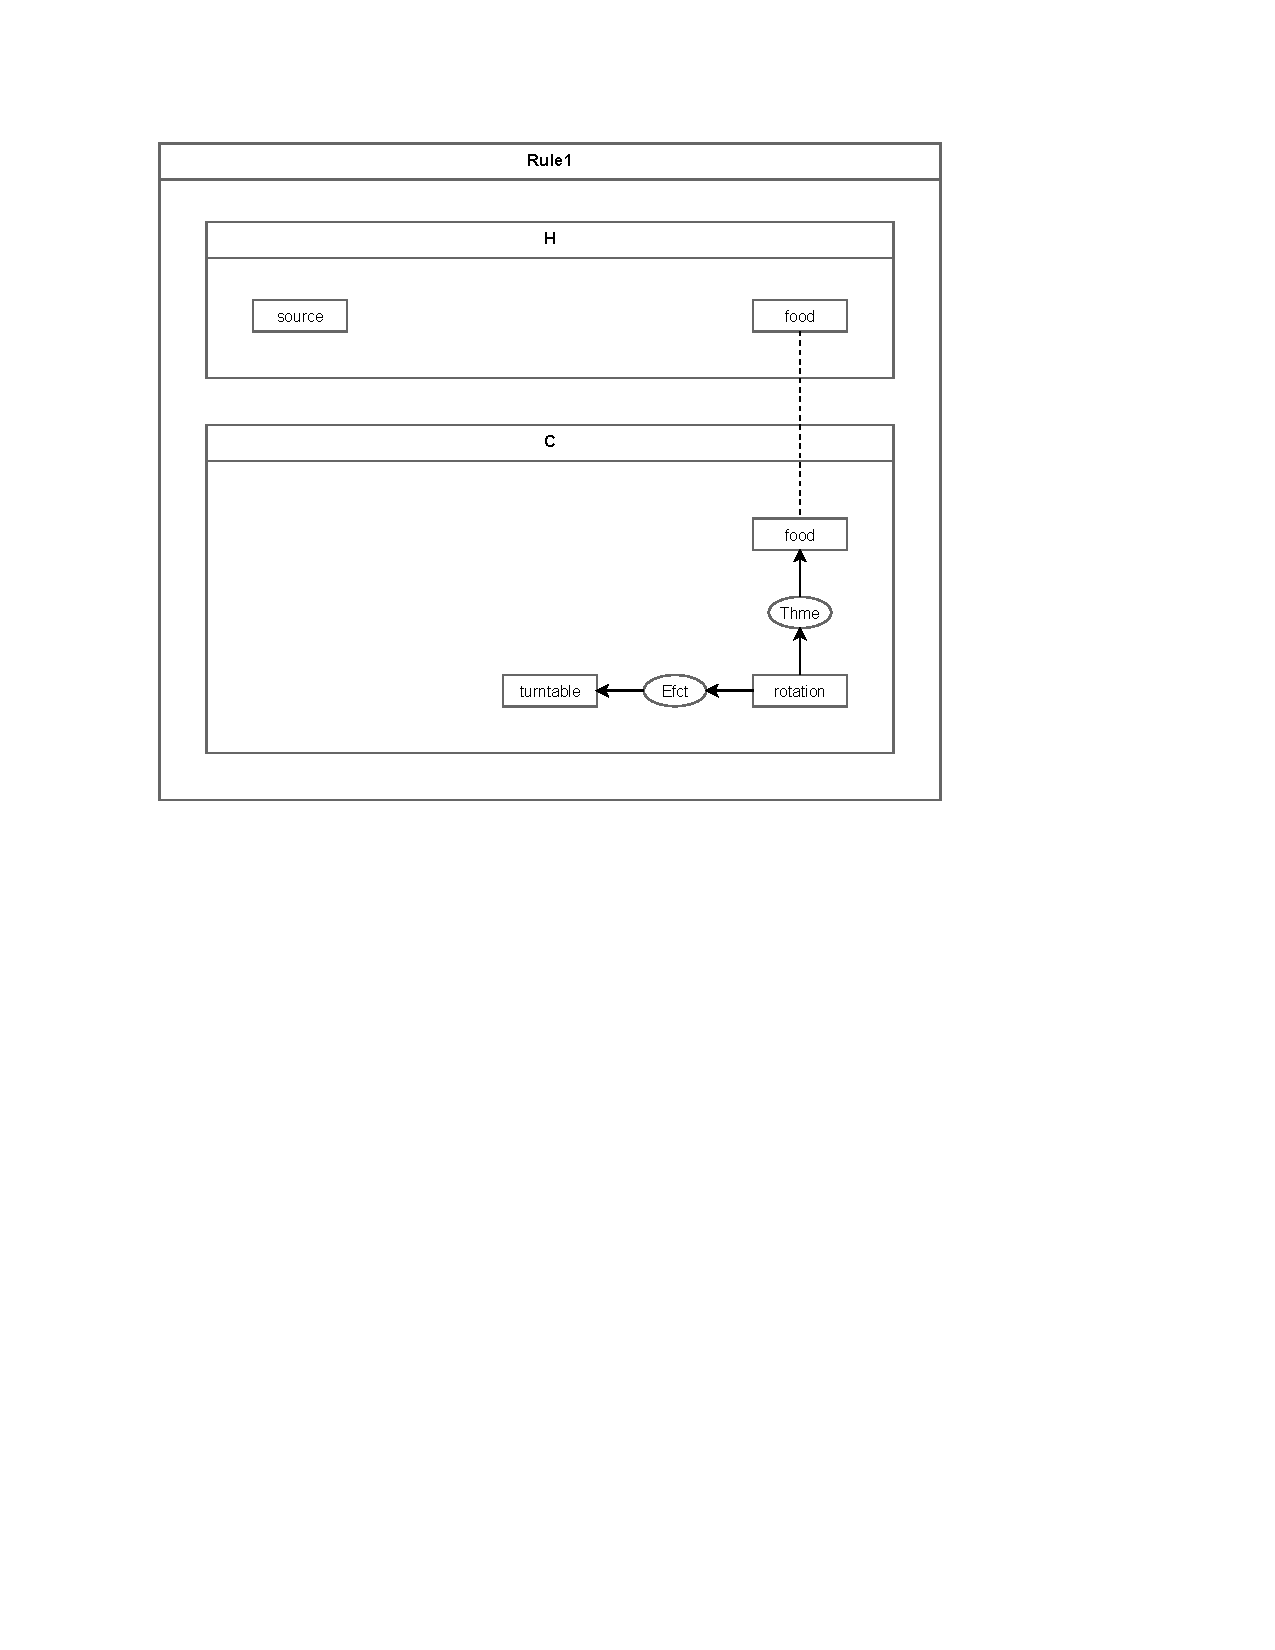
\includegraphics[width=0.70\textwidth]{./figures/wf_rule1.pdf} \end{center}

\setlength{\parindent}{0pt}
\rule{\textwidth}{1pt}
In the above rule, we notice an anomaly: `source' is {\em orphaned}. It appears in $H$, but not in $C$. It is cause for concern, and prompts review. We redesign the hypothesis graph, as shown below, to reflect relative motion between the source and food and deal with the orphaned concept.
\setlength{\parindent}{\mylength}

\begin{center} 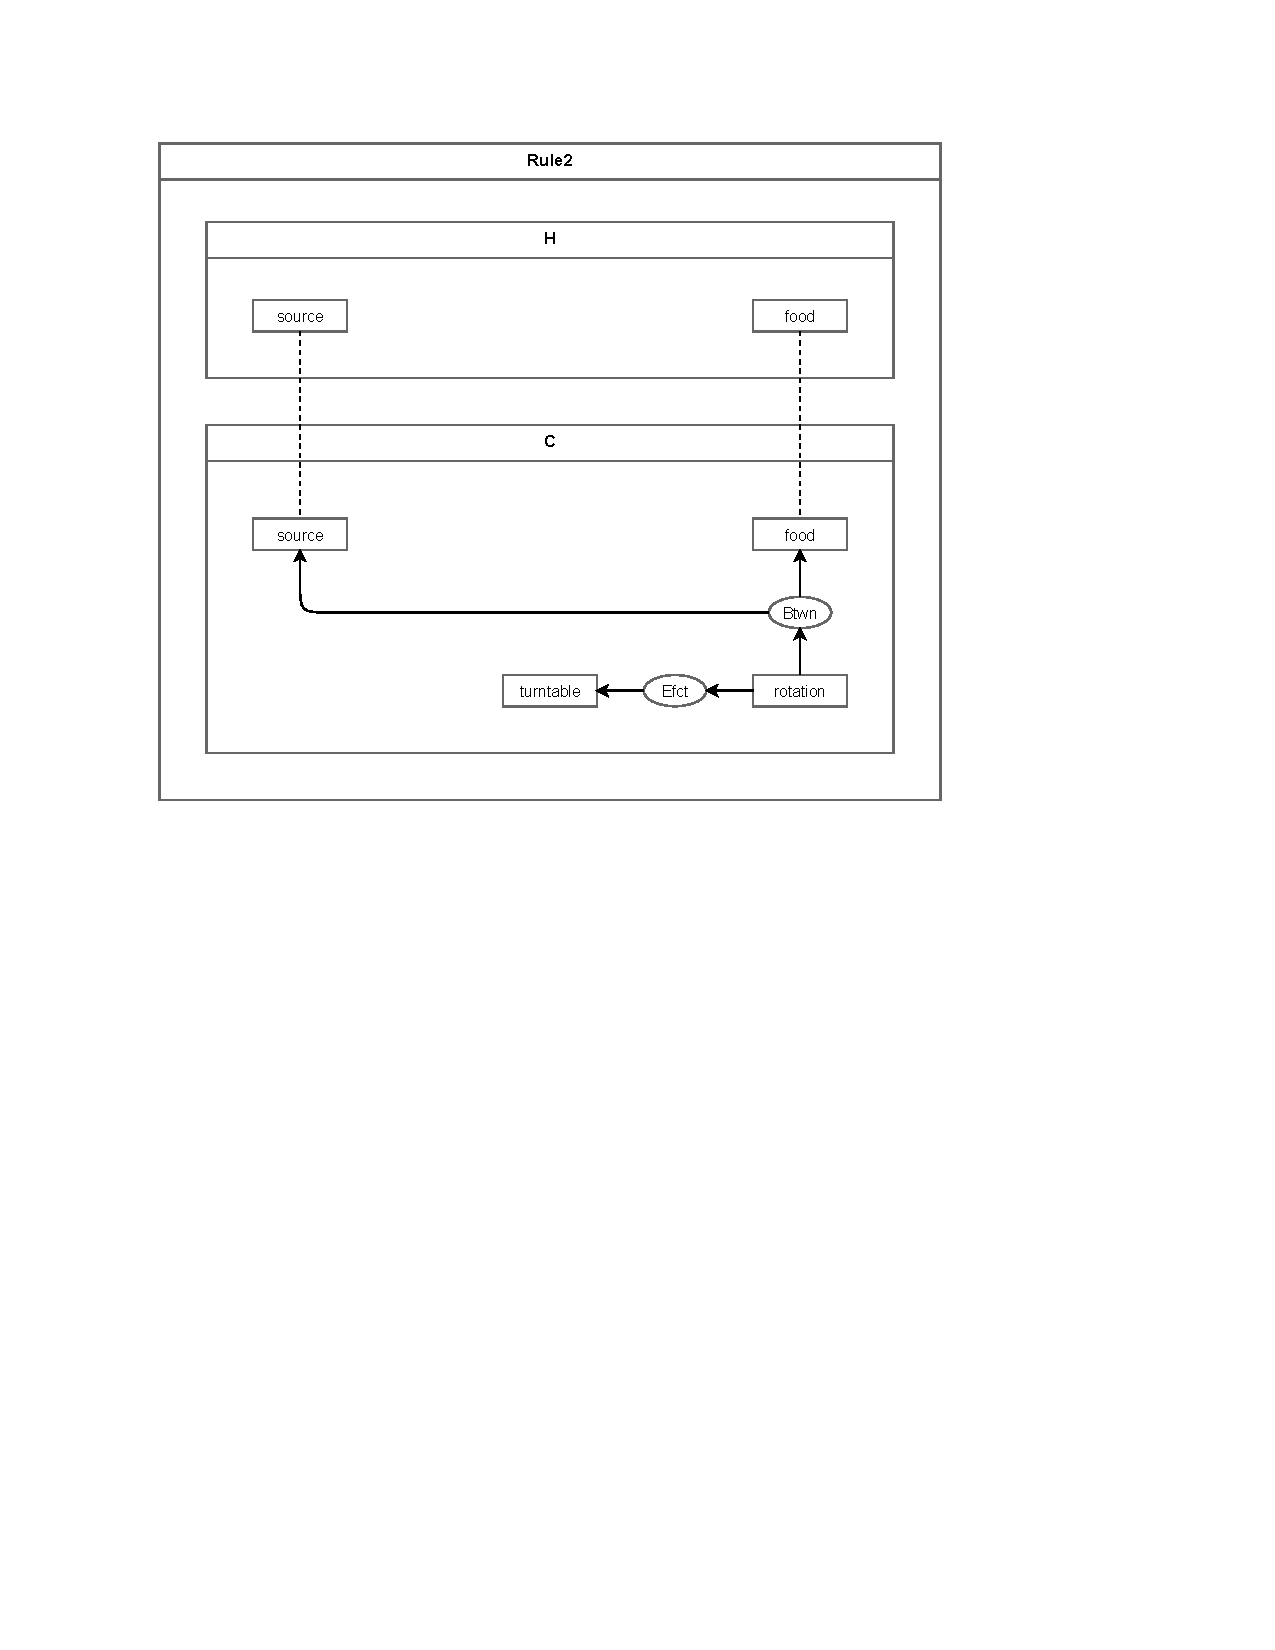
\includegraphics[width=0.70\textwidth]{./figures/wf_rule2.pdf} \end{center}

\setlength{\parindent}{0pt}
\rule{\textwidth}{1pt}
Next we consider a ``far-fetched'' embodiment to test our rule (i.e., claim). The embodiment below asserts that the food in the cavity is moved around by monkeys (suitably protected). Subsequently, we find a problem: although $H$ projects into this embodiment (i.e., the inventive step could be applied in this context), $C$ does not. In other words, the far-fetched embodiment contains inventive essence that is not captured by the rule.
\setlength{\parindent}{\mylength}

\begin{center} 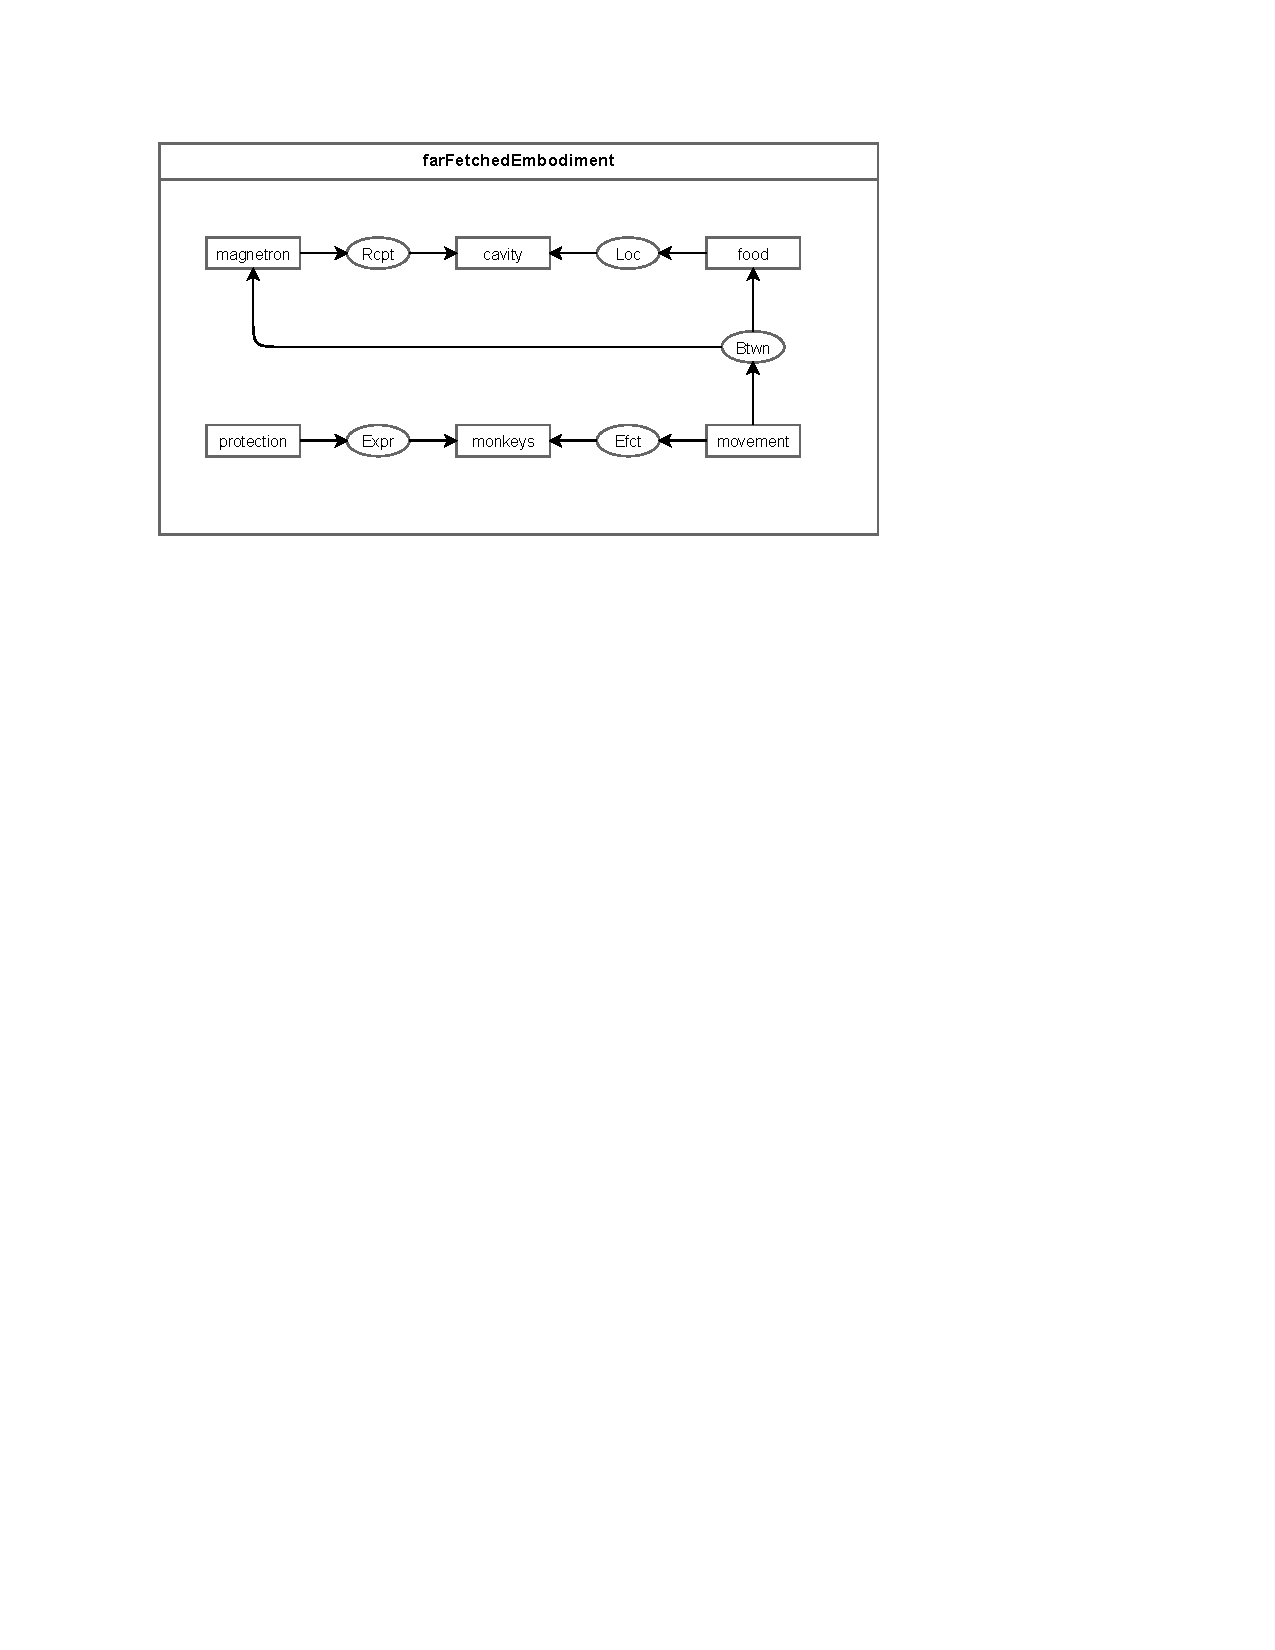
\includegraphics[width=0.70\textwidth]{./figures/wf_emb_ff.pdf} \end{center}

\setlength{\parindent}{0pt}
\rule{\textwidth}{1pt}
Our next step is to draw a conclusion graph for the far-fetched embodiment, as shown below.
\setlength{\parindent}{\mylength}

\begin{center} 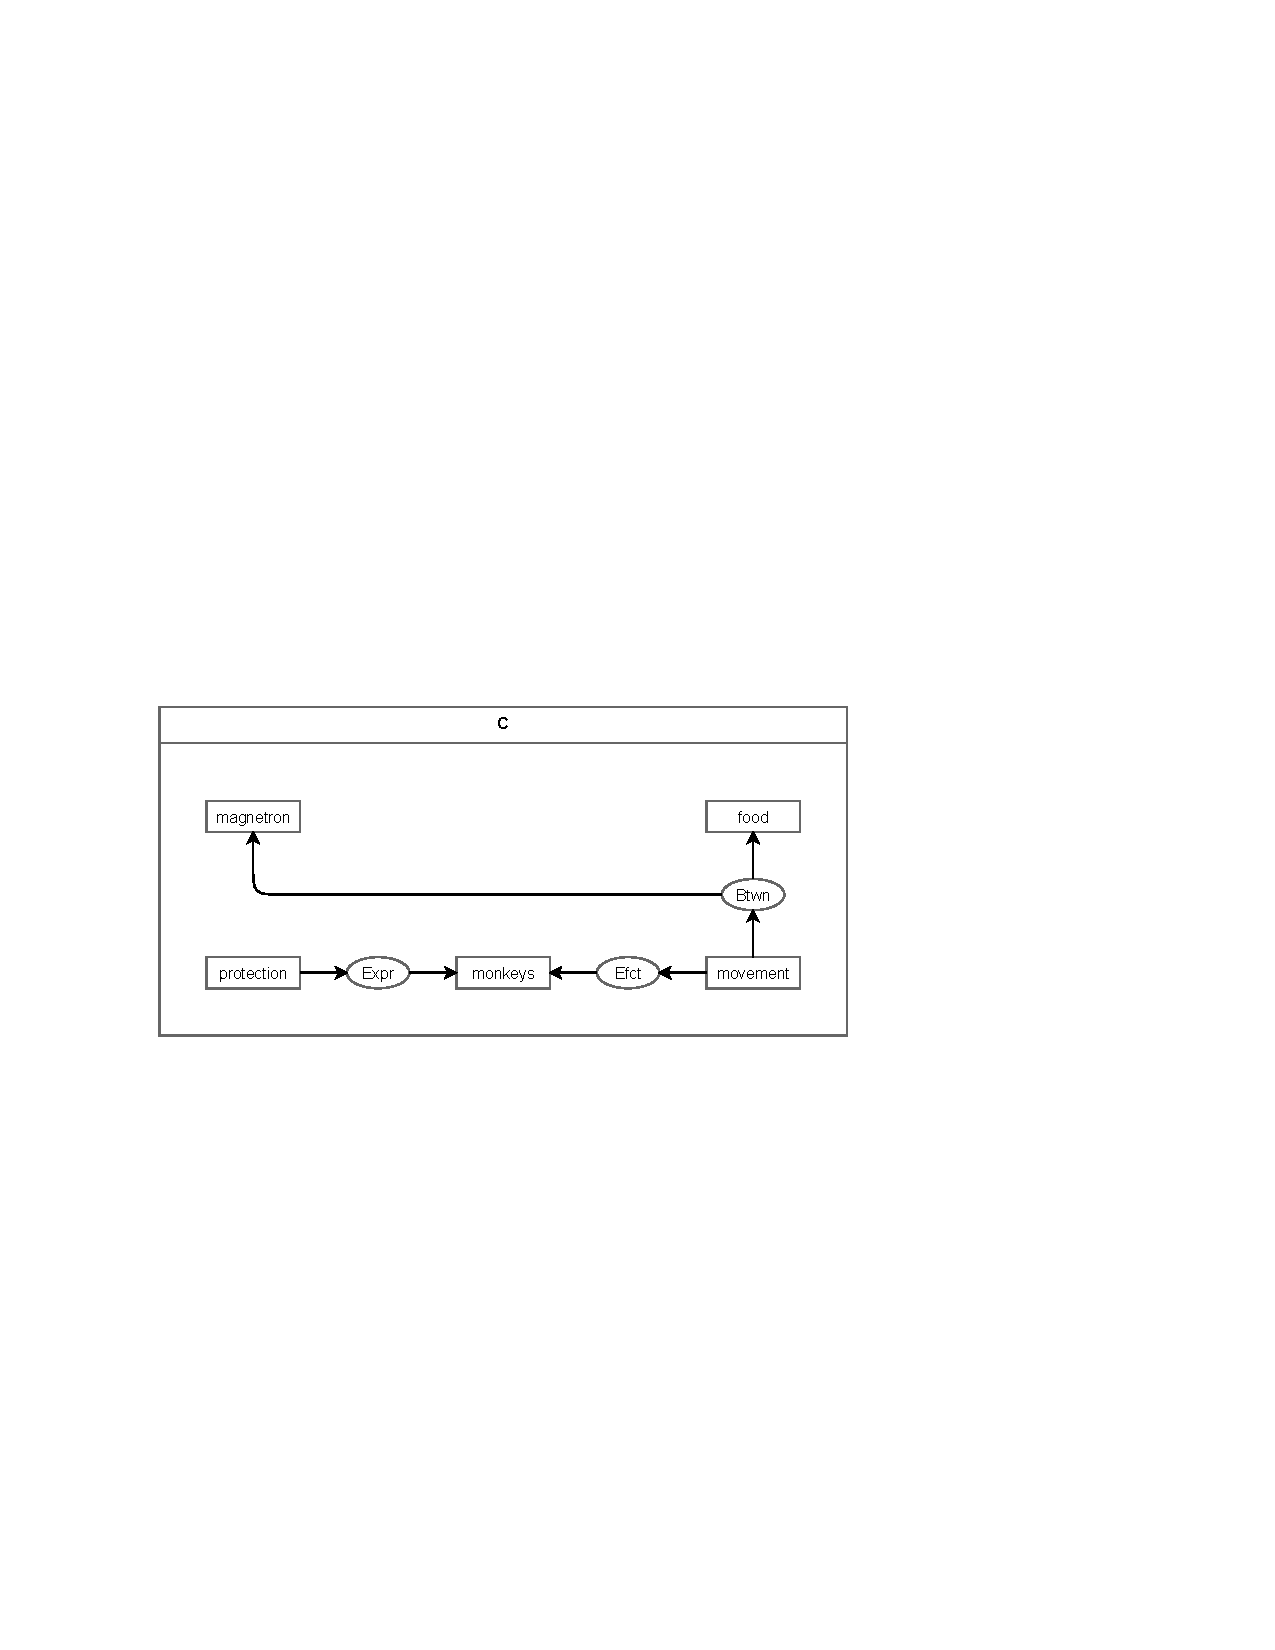
\includegraphics[width=0.70\textwidth]{./figures/wf_C1.pdf} \end{center}

\setlength{\parindent}{0pt}
\rule{\textwidth}{1pt}
Now, we may combine the inventive aspects of our original conclusion graph and the far-fetched conclusion graph using a the CG operation of `least-generalization' (see section~\ref{sec:leastgen}). The conclusion in the updated rule below shows the least-generalized conclusion.
\setlength{\parindent}{\mylength}

\begin{center} 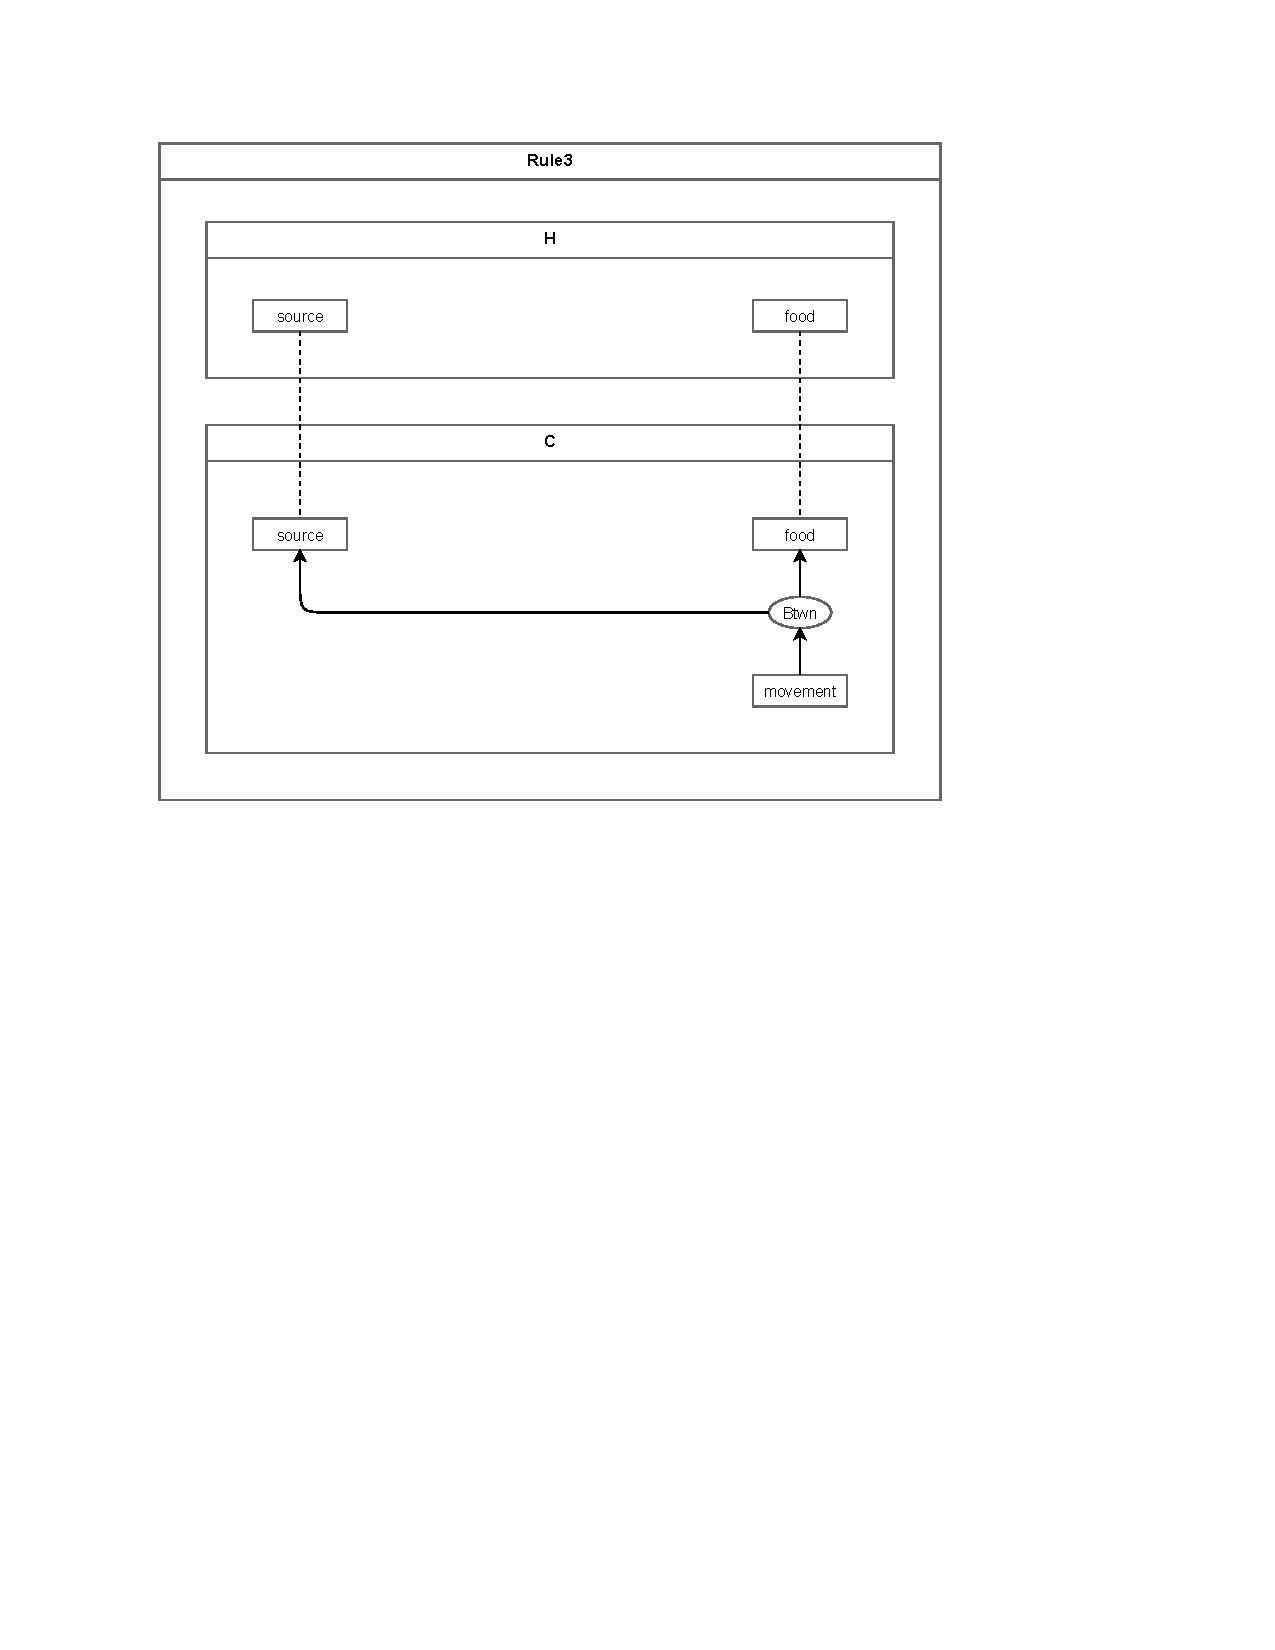
\includegraphics[width=0.70\textwidth]{./figures/wf_rule3.pdf} \end{center}

\setlength{\parindent}{0pt}
\rule{\textwidth}{1pt}
We now consider additional prior art: an infrared (`source:IR') rotisserie chicken roaster, as shown below. Since both the hypothesis and conclusion of our revised claim project into this prior art (i.e., the claim reads on the prior art), we must further revise our claim.
\setlength{\parindent}{\mylength}

\begin{center} 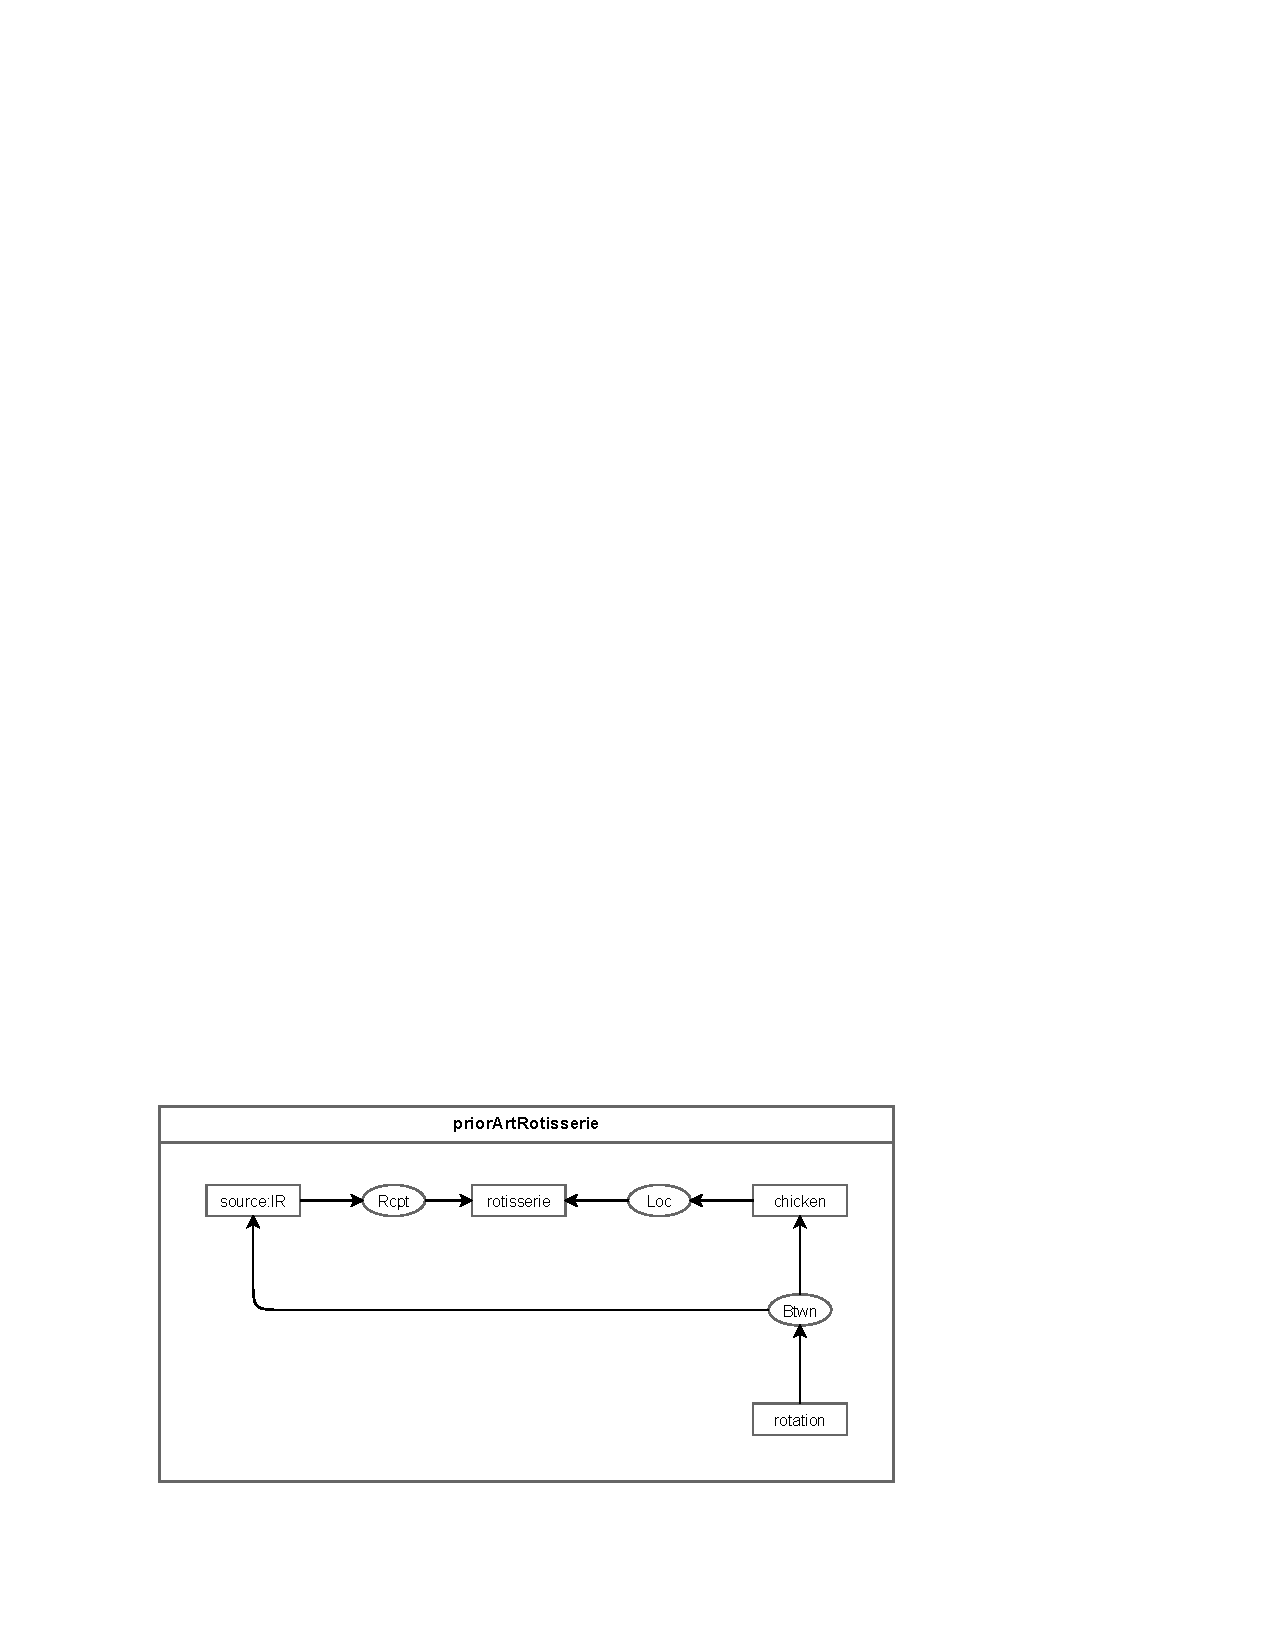
\includegraphics[width=0.70\textwidth]{./figures/wf_pa3.pdf} \end{center}

\setlength{\parindent}{0pt}
\rule{\textwidth}{1pt}
Rather than modifying (i.e., specializing) the conclusion (i.e., the inventive step), we instead change the hypothesis graph. The graph below shows H modified to include the cavity. Now, since H does not project into the prior art, our new claim is saved.
\setlength{\parindent}{\mylength}

\begin{center} 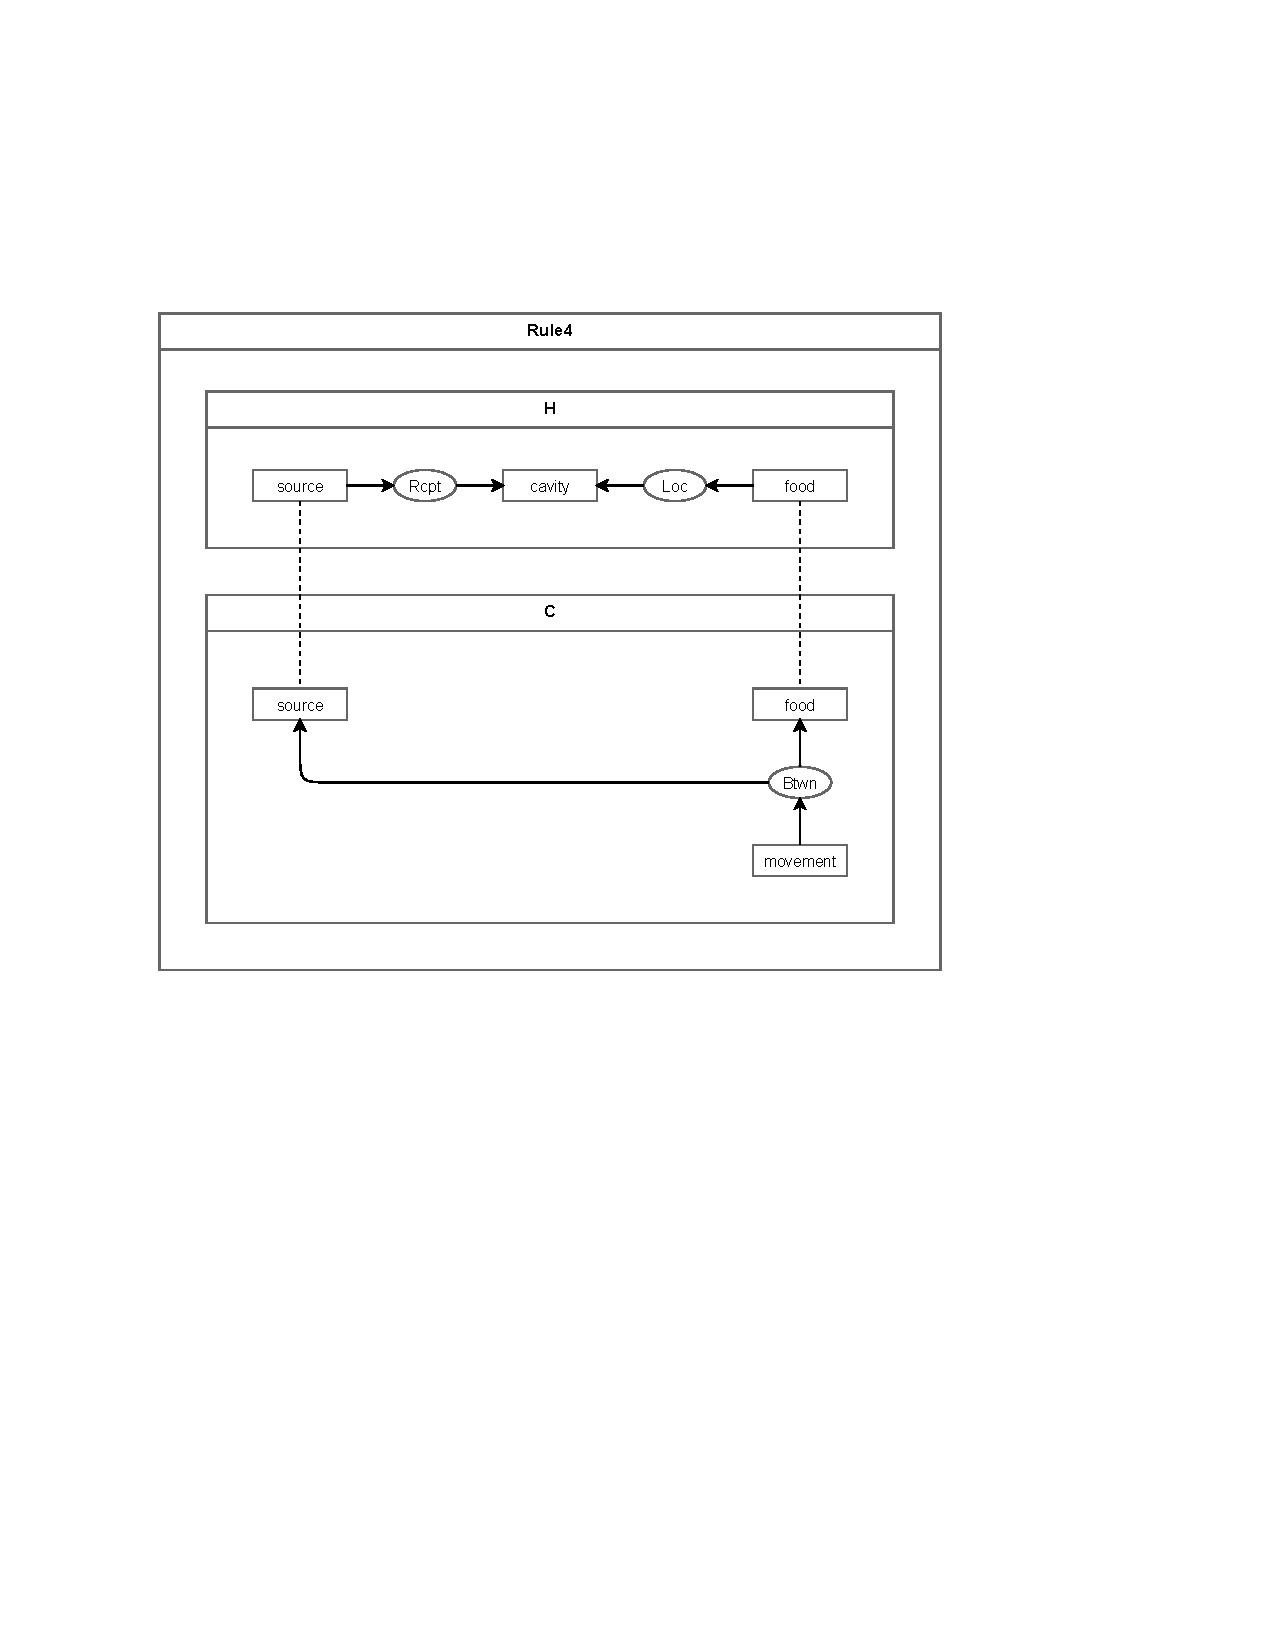
\includegraphics[width=0.70\textwidth]{./figures/wf_rule4.pdf} \end{center}

\setlength{\parindent}{0pt}
\rule{\textwidth}{1pt}
To conclude the claim, we generalize (un-restrict) `food' to `semi' (a semi, or partially, conducting material).
\setlength{\parindent}{\mylength}

\begin{center} 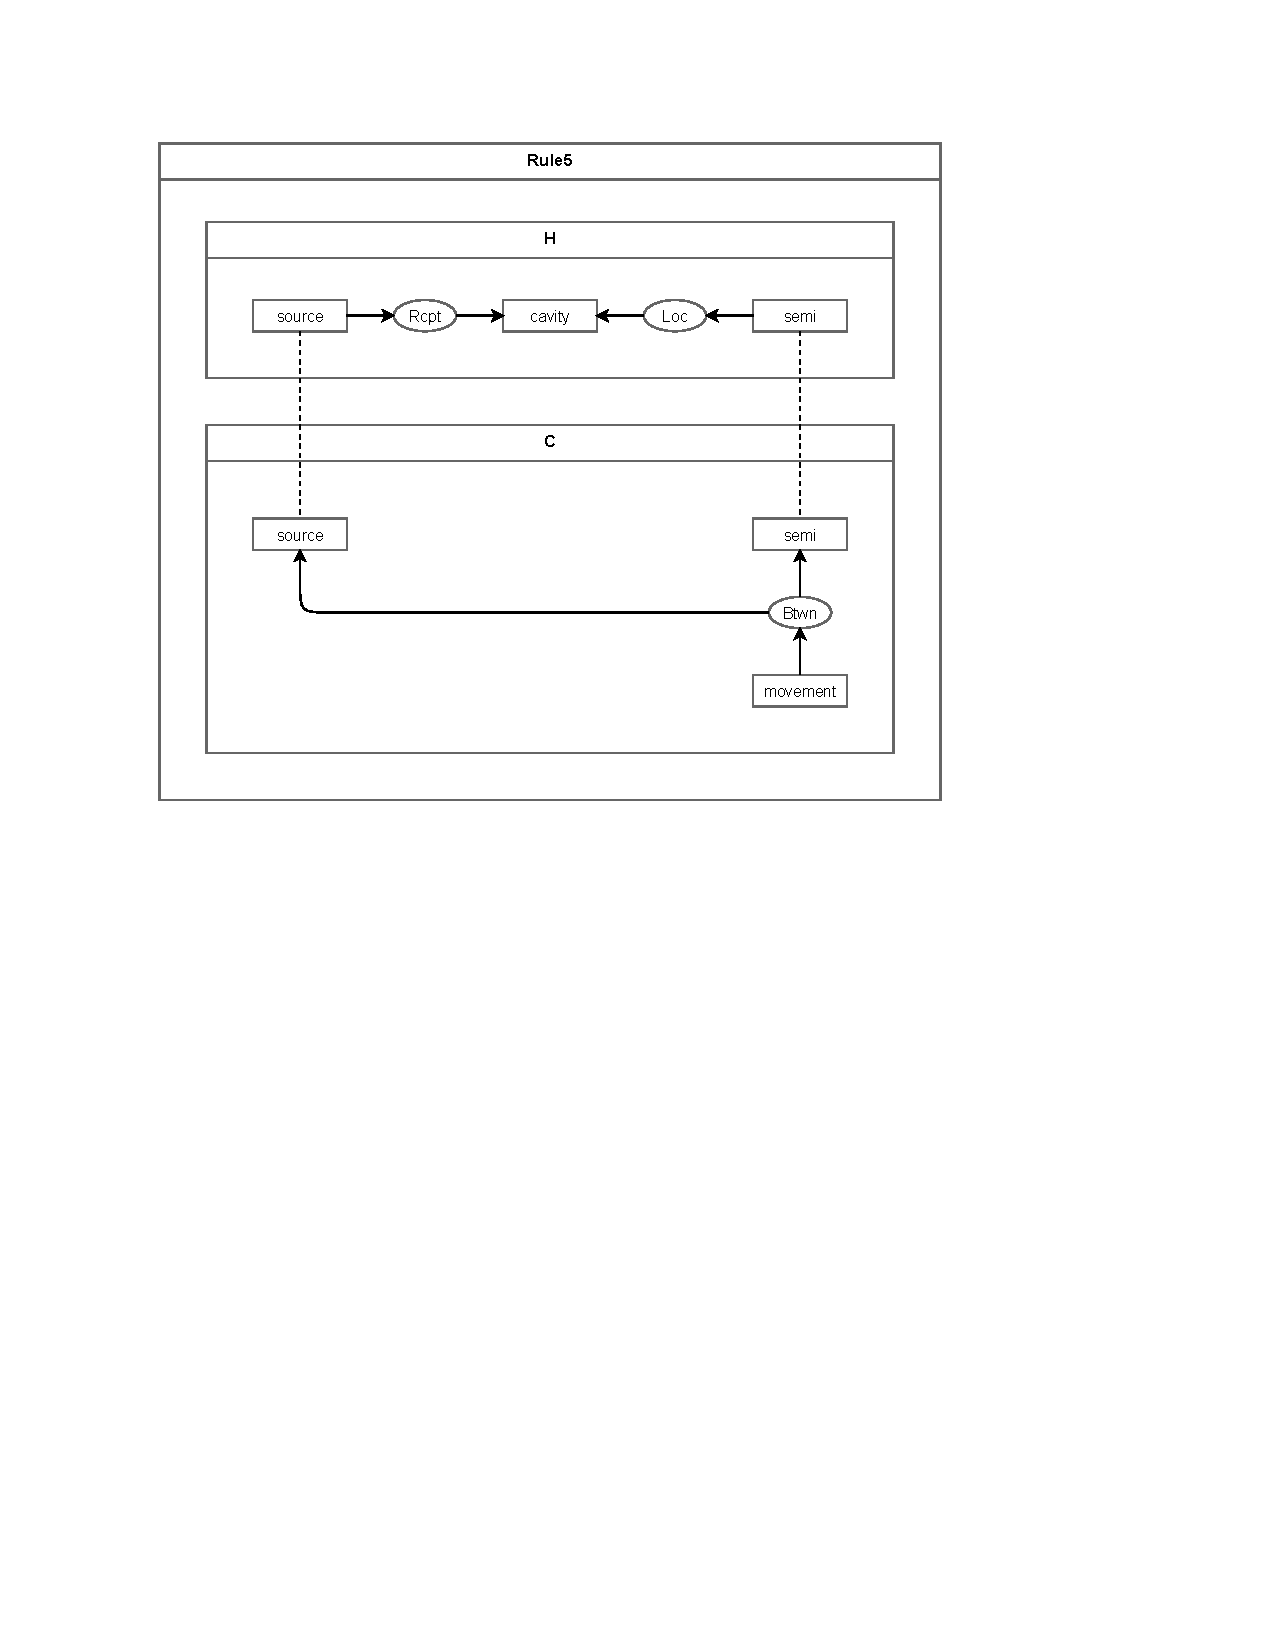
\includegraphics[width=0.70\textwidth]{./figures/wf_rule5.pdf} \end{center}

\setlength{\parindent}{0pt}
\rule{\textwidth}{1pt}
Finally, having settled the analysis of the invention and claim, we turn to designing the patent draft. Basically, we assign relevant subgraphs from the embodiments, prior art, and claims to relevant sections of the design. For instance, the graph below shows part of the design for the background section (populated with subgraphs from the prior art).
\setlength{\parindent}{\mylength}

\begin{center} 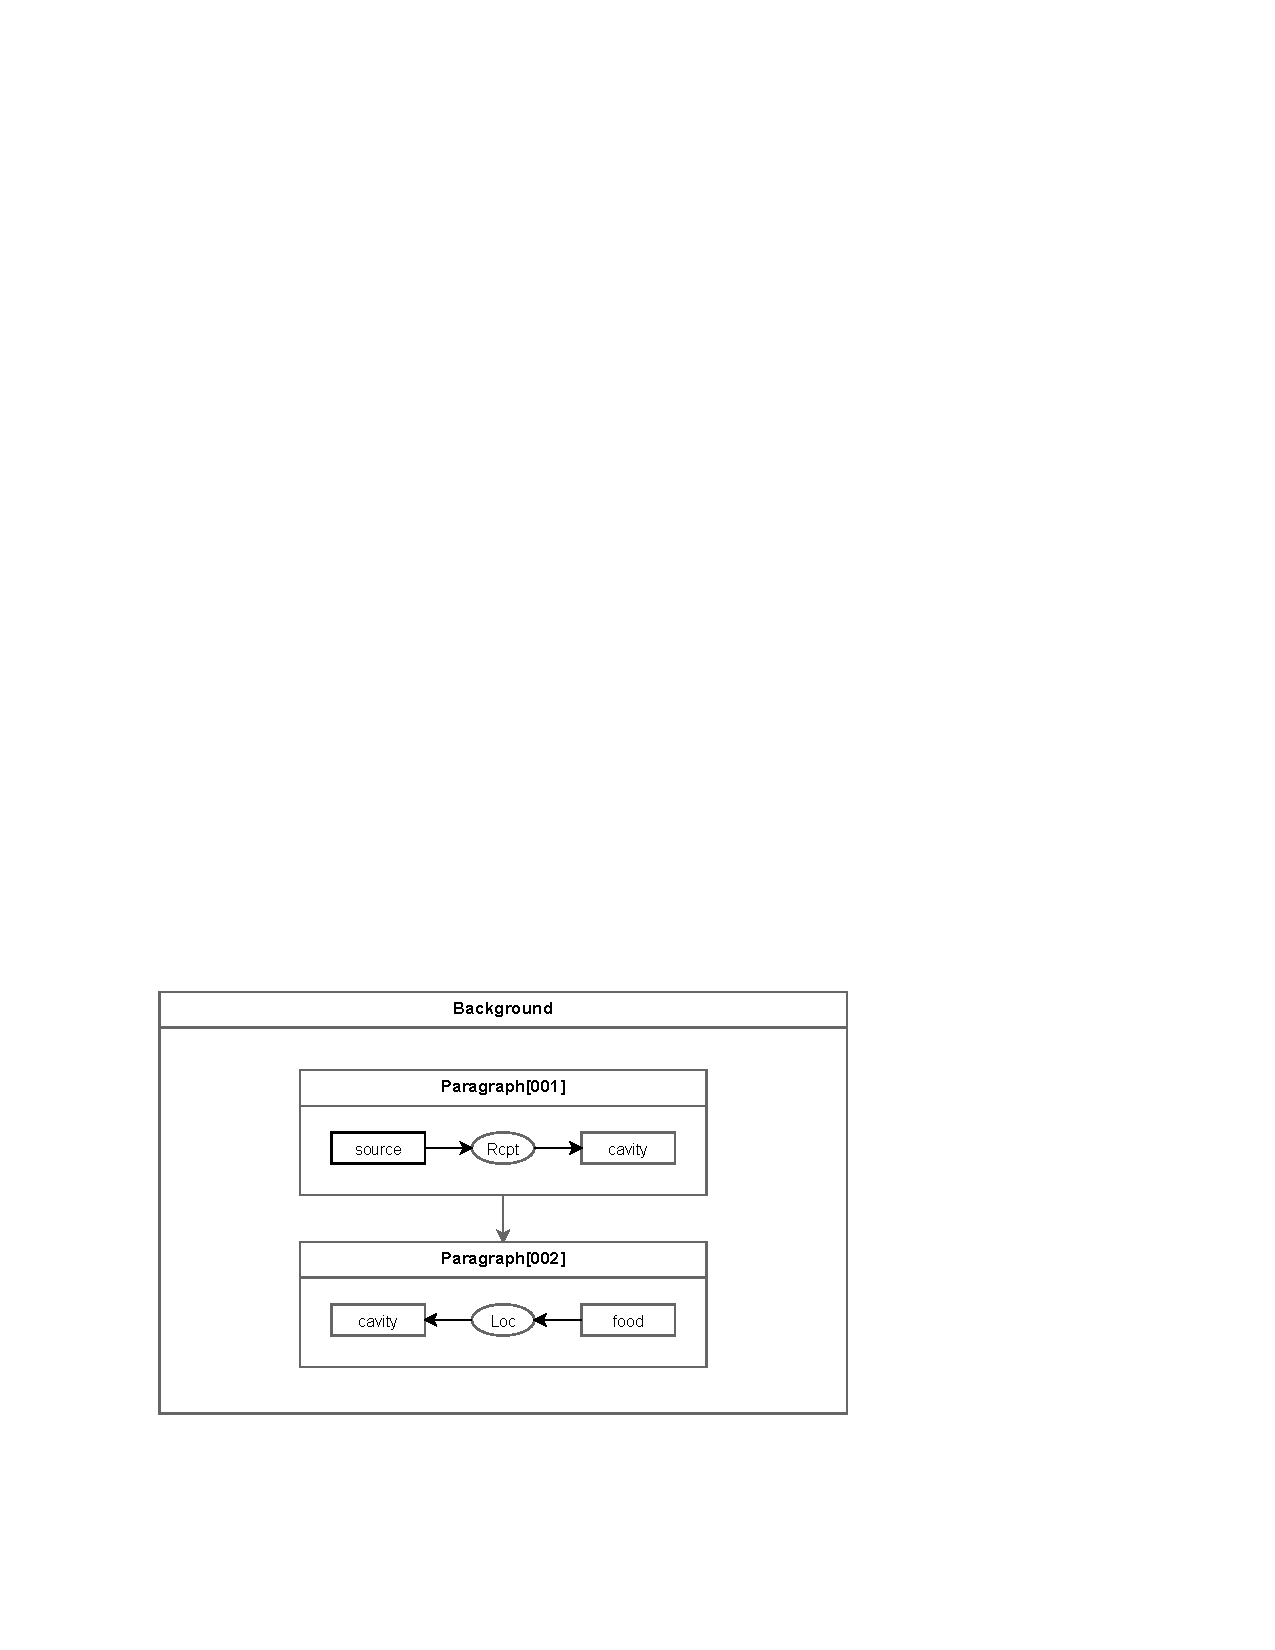
\includegraphics[width=0.70\textwidth]{./figures/background.pdf} \end{center}


\section{Correspondence between IACS and CGs}

\begin{table}[h]
\caption{Correspondence between IACS and CGs}
\label{tab:ideas}
\begin{tabularx}{\textwidth}{XX}
  \toprule
  IACS & CGs \\
  \hline
\\
  Inventions as concepts  & Graphical conceptual language \\[6pt]
  Particularizing element or relation & Specialization: restrict \\[6pt]
  Adding element & Specialization: join \\ [6pt]
  Prune & Generalization: detach \\[6pt]
  Distill & Generalization: unrestrict \\[6pt]
  Reads-on & Projection \\[6pt]
  Novelty and Infringement & Projection \\[6pt]
  Obviousness & Maximal join \\[6pt]
  Problem-solution statement & Rule \\[6pt]
  Claim & Rule \\[6pt]
  Broadest claim & Least-generalization \\[6pt]
  Fallback claim & Specialized chained rule \\[6pt]
  Inventive Departure & Conclusion graph \\[6pt]
  Definition Claim & Nested graph \\[6pt]
  Independent embodiment claim & Independent chained rule\\
\\
\bottomrule
\end{tabularx}
\end{table}

\newpage

\section{Biographies}

\setlength{\parindent}{0pt}
\textsc{Gary Ballantyne}


\rule[3mm]{\textwidth}{1pt}
\setlength{\parindent}{\mylength}
\vspace*{-0.8cm}

Dr. Ballantyne lives in Christchurch, New Zealand and is a founder of Haulashore Limited (a company based in Nelson, New Zealand). He has more than fifteen years experience in the wireless industry, most recently employed in the RF engineering department of Qualcomm Inc. where he was an expert in investigating, designing and developing advanced radio frequency (RF) system solutions. Dr. Ballantyne is a prolific inventor and has published numerous articles in the field of RF system design. Dr. Ballantyne has broad knowledge of wireless communications systems (with specific expertise at the physical layer), digital signal processing, and control systems.

\vspace*{0.5cm}

{\bf Education}

\begin{itemize}
\item
Ph.D, Electronic Engineering, University of Canterbury, 1994.
\item
B.E. (Hons), Electronic Engineering, University of Canterbury, 1991.
\end{itemize}

{\bf Patents and Publications}

\begin{itemize}
\item
10 granted US patents
\item
9 published US patent applications
\item
13 unpublished US patent applications
\item
7 refereed journal publications
\end{itemize}

\vspace*{0.25cm}
\setlength{\parindent}{0pt}
\textsc{Martin V. Clark}

\rule[3mm]{\textwidth}{1pt}
\setlength{\parindent}{\mylength}
\vspace*{-0.8cm}

Dr. Clark lives in Nelson, New Zealand and is a founder of Haulashore Limited. He has over 20 years experience in wireless communications. From 1992 to 1994, he worked at Telecom Corporation of New Zealand in the area of wireless technology analysis and modeling. He joined AT\&T Bell Laboratories in 1994, and AT\&T Labs in 1996 as a principal member of technical staff in the Wireless Communications Research Department. From 2002 to 2008, he worked at The MathWorks in the software development organization, including four years as manager of industry pilot projects for signal processing and communications. In the area of model-based design, he has collaborated with dozens of leading companies in communications, semiconductor, and aerospace/defense industries throughout North America, Europe, and Asia.

\vspace*{0.5cm}

{\bf Education}

\begin{itemize}
\item
Ph.D, Electronic Engineering, University of Canterbury, 1992.
\item
B.E. (Hons), Electronic Engineering, University of Canterbury, 1988.
\end{itemize}

{\bf Patents and Publications}

\begin{itemize}
\item
3 granted US patents
\item
2 published US patent applications
\item
4 unpublished US patent applications
\item
10 refereed journal publications
\end{itemize}

\vspace*{0.25cm}
\setlength{\parindent}{0pt}
\textsc{Adam Lins}

\rule[3mm]{\textwidth}{1pt}
\setlength{\parindent}{\mylength}
\vspace*{-0.8cm}

Mr. Lins lives in Martinez, United States of America and is a software developer for Haulashore Limited. He has over fifteen years experience writing and optimizing software for embedded processors used in digital signal processing applications. Mr. Lins also has broad experience in many areas of software development and application performance analysis. Most recently, Mr. Lins has collaborated on the design and development of a novel multi-processor architecture and associated tools and applications.

\vspace*{0.5cm}

{\bf Education}

\begin{itemize}
\item
M.E., Electronic Engineering, University of Canterbury, 1994.
\item
B.E., Electronic Engineering, University of Canterbury, 1993.
\end{itemize}


%You shouldn't write {\em anything} first. Figure out what the invention is, and then you can write whatever you want.
%
%For patent lawyers, however, an invention is not something physical, but a concept.
%
%A conceptual graph (CG) is a graph representation for logic based on the semantic networks
%of artificial intelligence and the existential graphs of Charles Sanders Peirce.
%
%Problem-solution statement in hand, the patent attorney can begin his claim drafting not with an empty screen, but with a substantial essence of inventive essence.
%
%In accordance with the original definition of the term "patent," patents facilitate and encourage disclosure of innovations into the public domain for the common good.
%
%Logic will get you from A to B. Imagination will take you everywhere.

\end{document}
